\documentclass[12pt,a4paper]{report}

% ==================== COUNTERS ====================
\setcounter{secnumdepth}{4}
\setcounter{tocdepth}{4}

% ==================== PACKAGES ====================
\usepackage[utf8]{inputenc}
\usepackage{cite}
\usepackage{times}

\usepackage{cite}
\usepackage{longtable}
\bibliographystyle{IEEEtran}
\usepackage{geometry}
\usepackage{setspace}
\usepackage{graphicx}
\usepackage{float}
\usepackage{titlesec}
\usepackage[titles]{tocloft}
\usepackage{fancyhdr}
\usepackage{hyperref}
\usepackage{amsmath,amssymb}
\usepackage{booktabs}
\usepackage{longtable}
\usepackage{caption}
\usepackage{subcaption}
\usepackage{listings}
\usepackage{xcolor}
\usepackage{enumitem}
\usepackage[normalem]{ulem}

% ==================== PAGE SETUP ====================
\geometry{
	a4paper,
	left=1.5in,
	right=1in,
	top=1in,
	bottom=1.2in
}

% ==================== FORMATTING: TOC & LISTS ====================
\renewcommand{\contentsname}{TABLE OF CONTENTS}
\renewcommand{\cfttoctitlefont}{\hfill\Large\bfseries}
\renewcommand{\cftaftertoctitle}{\hfill}

\renewcommand{\listfigurename}{LIST OF FIGURES}
\renewcommand{\cftloftitlefont}{\hfill\Large\bfseries}
\renewcommand{\cftafterloftitle}{\hfill}

\renewcommand{\listtablename}{LIST OF TABLES}
\renewcommand{\cftlottitlefont}{\hfill\Large\bfseries}
\renewcommand{\cftafterlottitle}{\hfill}

\renewcommand{\cftfigpresnum}{Figure }
\setlength{\cftfignumwidth}{6.5em}
\renewcommand{\cftfigfont}{\itshape}
\renewcommand{\cftfigleader}{\cftdotfill{\cftdotsep}}

\renewcommand{\cfttabpresnum}{Table }
\setlength{\cfttabnumwidth}{6em}
\renewcommand{\cfttabfont}{\itshape}
\renewcommand{\cfttableader}{\cftdotfill{\cftdotsep}}

\renewcommand{\cftchapleader}{\cftdotfill{\cftdotsep}}

% ==================== LINE SPACING ====================
% Front matter: single spacing (applied locally)
% From Chapter 1 onwards: 1.5 spacing (applied via \onehalfspacing below main content)
\onehalfspacing

% ==================== PARAGRAPH SPACING ====================
% Template: spacing before and after paragraph = 6 points (from Chapter 1 onwards)
% Applied via \setlength after \pagenumbering{arabic} in document body

% ==================== HYPERREF ====================
\hypersetup{
	colorlinks=true,
	linkcolor=black,
	urlcolor=blue,
	citecolor=black,
	pdftitle={User-Friendly Autonomous Parcel Delivery System},
	pdfauthor={Muhammad Ali Hassan, Aitzaz Arshad, Gulfam Haider}
}

% ==================== EQUATION NUMBERING ====================
% Format: (Eq X.Y) where X = chapter number, Y = sequence within chapter
\renewcommand{\theequation}{Eq \thechapter.\arabic{equation}}

% ==================== HEADINGS FORMATTING ====================
% Per template:
% Chapter label:  font 18, bold, sentence case, left-aligned, spacing before 6pt after 24pt
% Chapter title:  font 18, bold, ALL CAPS, center-aligned, spacing before 6pt after 24pt
% Section:        font 16, bold, Title Case, left-aligned, spacing before/after 6pt
% Subsection:     font 14, Title Case, left-aligned, spacing before/after 6pt
% Subsubsection:  font 12, Underlined, Sentence case, left-aligned, spacing before/after 6pt

\titlespacing*{name=\chapter,numberless}{0pt}{-20pt}{18pt}

\titleformat{\chapter}[display]
{\normalfont\bfseries\fontsize{18}{22}\selectfont}
{Chapter \thechapter}
{6pt}
{\centering\MakeUppercase}

\titlespacing*{\chapter}{0pt}{-10pt}{24pt}

\titleformat{\section}
{\normalfont\fontsize{16}{19}\bfseries}
{\thesection}{1em}{}
\titlespacing*{\section}{0pt}{6pt}{6pt}

\titleformat{\subsection}
{\normalfont\fontsize{14}{17}\bfseries}
{\thesubsection}{1em}{}
\titlespacing*{\subsection}{0pt}{6pt}{6pt}

% Subsubsection: font 12, underlined, sentence case
% \uline must go in the 5th (before-code) argument, not the format argument
\titleformat{\subsubsection}
{\normalfont\fontsize{12}{15}\selectfont}
{\thesubsubsection}{1em}{\uline}
\titlespacing*{\subsubsection}{0pt}{6pt}{6pt}

% ==================== HEADER / FOOTER ====================
\pagestyle{fancy}
\fancyhf{}
\fancyfoot[R]{\thepage}
\renewcommand{\headrulewidth}{0pt}
\renewcommand{\footrulewidth}{0pt}

\fancypagestyle{plain}{
	\fancyhf{}
	\fancyfoot[R]{\thepage}
	\renewcommand{\headrulewidth}{0pt}
	\renewcommand{\footrulewidth}{0pt}
}

% ==================== CODE LISTINGS ====================
\lstset{
	basicstyle=\fontfamily{pcr}\selectfont\fontsize{10}{12},
	breaklines=true,
	frame=single,
	numberstyle=\tiny,
	captionpos=b
}

% ==================== VARIABLES ====================
\newcommand{\projecttitle}{USER-FRIENDLY AUTONOMOUS PARCEL DELIVERY SYSTEM WITH ADAPTIVE NAVIGATION}
\newcommand{\studentonename}{Muhammad Ali Hassan}
\newcommand{\studentonereg}{BEE223007}
\newcommand{\studenttwoname}{Aitzaz Arshad}
\newcommand{\studenttworeg}{BEE223010}
\newcommand{\studentthreename}{Gulfam Haider}
\newcommand{\studentthreereg}{BEE223020}
\newcommand{\supervisorname}{Engr. Suleman Khan}
\newcommand{\supervisortitle}{Lecturer}
\newcommand{\cosupervisorname}{Dr. Muhammad Atif}
\newcommand{\cosupervisortitle}{Managing AI Director}
\newcommand{\hodname}{Dr. Noor Mohammad Khan}
\newcommand{\hodtitle}{Professor}
\newcommand{\submissionmonth}{July}
\newcommand{\submissionyear}{2026}

\begin{document}
	
	% ==================== TITLE PAGE ====================
	\begin{titlepage}
		\begin{center}
			{\fontsize{20}{24}\selectfont\bfseries\MakeUppercase{\projecttitle}\par}
			\vspace{1cm}
			
\includegraphics[width=1.7in]{logo.png}
			\vspace{1cm}
			
			{\fontsize{14}{17}\selectfont by\par}
			\vspace{0.5cm}
			
			{\fontsize{16}{19}\selectfont\studentonename\par}
			{\fontsize{15}{18}\selectfont\studentonereg\par}
			\vspace{0.3cm}
			
			{\fontsize{16}{19}\selectfont\studenttwoname\par}
			{\fontsize{15}{18}\selectfont\studenttworeg\par}
			\vspace{0.3cm}
			
			{\fontsize{16}{19}\selectfont\studentthreename\par}
			{\fontsize{15}{18}\selectfont\studentthreereg\par}
			
			\vspace{1cm}
			
			{\fontsize{14}{17}\selectfont
				A Project Report submitted to the\\
				DEPARTMENT OF ELECTRICAL AND COMPUTER ENGINEERING\\
				in partial fulfillment of the requirements for the degree of\\
				BACHELOR OF SCIENCE IN ELECTRICAL ENGINEERING
			}
			
			\vspace{1cm}
			
			{\fontsize{14}{17}\selectfont
				Faculty of Engineering\\
				Capital University of Science \& Technology, Islamabad
			}
			
			\vspace{1cm}
			
			{\fontsize{14}{17}\selectfont\submissionmonth, \submissionyear}
		\end{center}
	\end{titlepage}
	
	% ==================== FRONT MATTER ====================
	% Template: front matter uses SINGLE line spacing
	\singlespacing
	\pagenumbering{roman}
	\setcounter{page}{2}
	
	% --- Copyright ---
	\thispagestyle{plain}
	\begin{center}
		{\fontsize{12}{14}\selectfont
			Copyright \textcopyright\ \submissionyear\ by CUST Students
			
			\vspace{0.5cm}
			
			All rights reserved. Reproduction in whole or in part in any form requires prior written permission of
			\studentonename, \studenttwoname\ and \studentthreename.
		}
	\end{center}
	\clearpage
	\chapter*{Confidentiality Statement}
	\addcontentsline{toc}{chapter}{Confidentiality Statement}
	
	This report is submitted solely for the purpose of Final Year Project academic evaluation. The project has been developed under the supervision of EIOTAI and is subject to a Non-Disclosure Agreement (NDA).
	\newpage
	% --- Declaration ---
	\chapter*{DECLARATION}
	\addcontentsline{toc}{chapter}{DECLARATION}
	\thispagestyle{plain}
	
	It is declared that this is an original piece of our work, except where otherwise acknowledged in text and references. This work has not been submitted in any form for another degree or diploma at any university or other institution for tertiary education and shall not be submitted by us in future for obtaining any degree from this or any other University or Institution.
	
	\vspace{2cm}
	
	\noindent
	\begin{tabular}{@{}l@{}}
		\studentonename \\
		\studentonereg
	\end{tabular}
	
	\vspace{1cm}
	
	\noindent
	\begin{tabular}{@{}l@{}}
		\studenttwoname \\
		\studenttworeg
	\end{tabular}
	
	\vspace{1cm}
	
	\noindent
	\begin{tabular}{@{}l@{}}
		\studentthreename \\
		\studentthreereg
	\end{tabular}
	
	\vspace{2cm}
	
	\noindent
	\submissionmonth\ \submissionyear
	\clearpage
	
	% --- Certificate ---
	\chapter*{CERTIFICATE OF APPROVAL}
	\addcontentsline{toc}{chapter}{CERTIFICATE OF APPROVAL}
	\thispagestyle{plain}
	
	It is certified that the project titled \textbf{``\projecttitle''} carried out by \studentonename, Reg. No. \studentonereg, \studenttwoname, Reg. No. \studenttworeg, and \studentthreename, Reg. No. \studentthreereg, under the supervision of \supervisorname\ and co-supervision of \cosupervisorname, Capital University of Science \& Technology, Islamabad, is fully adequate, in scope and in quality, as a final year project for the degree of BS Electrical Engineering.
	
	\vspace{1.5cm}
	
	\noindent\textbf{Supervisor:}
	\begin{center}
		\makebox[7cm]{\dotfill} \\
		\supervisorname \\
		\supervisortitle \\
		Department of Electrical and Computer Engineering \\
		Faculty of Engineering \\
		Capital University of Science \& Technology, Islamabad
	\end{center}
	
	\vspace{1cm}
	
	\noindent\textbf{Co-Supervisor:}
	\begin{center}
		\makebox[7cm]{\dotfill} \\
		\cosupervisorname \\
		\cosupervisortitle \\
		EIOTAI (Private) Limited
	\end{center}
	
	\vspace{1cm}
	
	\noindent\textbf{HoD:}
	\begin{center}
		\makebox[7cm]{\dotfill} \\
		\hodname \\
		\hodtitle \\
		Department of Electrical and Computer Engineering \\
		Faculty of Engineering \\
		Capital University of Science \& Technology, Islamabad
	\end{center}
	\clearpage
	
	% --- Acknowledgment ---
	\chapter*{ACKNOWLEDGMENT}
	\addcontentsline{toc}{chapter}{ACKNOWLEDGMENT}
	\thispagestyle{plain}
	
	We would like to express our sincere gratitude to our supervisor, \supervisorname, for his invaluable guidance, continuous support, and encouragement throughout this project. His expertise and insights have been instrumental in the successful completion of this work.
	
	We are deeply grateful to our co-supervisor, \cosupervisorname, Managing AI Director, for his expert advice, technical guidance, and support in the development and implementation of the autonomous navigation and AI components of this project.
	
	We would also like to extend our thanks to the faculty members of the Department of Electrical and Computer Engineering at Capital University of Science \& Technology for their assistance and valuable feedback during various stages of this project. Finally, we acknowledge our families and friends for their unwavering support and encouragement throughout our academic journey.
	\clearpage
	
	% --- Abstract ---
	\chapter*{ABSTRACT}
	\addcontentsline{toc}{chapter}{ABSTRACT}
	\thispagestyle{plain}

	The increasing demand for automation in hospitals, universities, offices, and other indoor environments has created a need for intelligent autonomous delivery systems capable of transporting parcels safely and efficiently with minimal human intervention. This project presents the design and implementation of a simulation-based autonomous indoor parcel delivery system using ROS 2 and the Gazebo simulation environment. The proposed system provides a complete software framework for autonomous navigation, parcel delivery management, and real-time user interaction without requiring physical robot hardware.
	A custom navigation framework was developed by integrating an Improved A* (IA*) algorithm for global path planning, path pruning to eliminate redundant waypoints, and Particle Swarm Optimization (PSO) to optimize the generated path. A Model Predictive Controller (MPC) was designed to accurately track the optimized trajectory while satisfying the kinematic constraints of a differential-drive mobile robot. To enable safe navigation in dynamic indoor environments, a Model Predictive Path Integral (MPPI) controller was incorporated as the local planner for real-time obstacle avoidance and local trajectory adaptation. The complete navigation framework was integrated with ROS 2, SLAM-based localization, occupancy grid mapping, RViz visualization, and Gazebo simulation. A Flutter-based web application with a Flask backend was also developed to allow users to submit delivery requests, monitor robot status in real time, manage indoor maps, and communicate with the ROS 2 navigation system through a web–ROS bridge. The proposed system was evaluated in multiple simulated indoor environments containing corridors, rooms, static obstacles, and moving pedestrians. Experimental results demonstrate that the integrated navigation framework successfully generates collision-free and optimized paths, accurately tracks the planned trajectory, and safely avoids dynamic obstacles while maintaining stable navigation performance. The developed web application provides an intuitive interface for delivery management and real-time robot monitoring, making the overall system modular, scalable, and suitable for future deployment on physical robotic platforms.The proposed system establishes a robust foundation for autonomous indoor logistics and can be extended to support real-world deployment, multi-robot coordination, and intelligent delivery applications in hospitals, warehouses, and academic institutions.
		\clearpage
	
	% ==================== TABLES OF CONTENTS ====================
	\tableofcontents
	\addcontentsline{toc}{chapter}{TABLE OF CONTENTS}
	\clearpage
	
	% ==================== LIST OF FIGURES ====================
	\listoffigures
	\addcontentsline{toc}{chapter}{LIST OF FIGURES}
	\clearpage
	
	% ==================== LIST OF TABLES ====================
	\listoftables
	\addcontentsline{toc}{chapter}{LIST OF TABLES}
	\clearpage
	
	% ==================== ACRONYMS ====================
	\chapter*{LIST OF ACRONYMS/ABBREVIATIONS}
	\addcontentsline{toc}{chapter}{LIST OF ACRONYMS/ABBREVIATIONS}
	\thispagestyle{plain}
\begin{longtable}{p{3.5cm} p{10cm}}
	AI      & Artificial Intelligence \\
	AMCL    & Adaptive Monte Carlo Localization \\
	API     & Application Programming Interface \\
	A*      & A-Star Path Planning Algorithm \\
	CPU     & Central Processing Unit \\
	DC      & Direct Current \\
	FSM     & Finite State Machine \\
	GPS     & Global Positioning System \\
	GUI     & Graphical User Interface \\
	IA*     & Improved A-Star Algorithm \\
	IMU     & Inertial Measurement Unit \\
	IoT     & Internet of Things \\
	JSON    & JavaScript Object Notation \\
	LiDAR   & Light Detection and Ranging \\
	MPC     & Model Predictive Control \\
	MPPI    & Model Predictive Path Integral \\
	Nav2    & Navigation 2 Framework \\
	NDA     & Non-Disclosure Agreement \\
	PID     & Proportional--Integral--Derivative \\
	PSO     & Particle Swarm Optimization \\
	ROS     & Robot Operating System \\
	ROS~2   & Robot Operating System 2 \\
	RRT     & Rapidly-Exploring Random Tree \\
	RViz    & Robot Visualization Tool \\
	SLAM    & Simultaneous Localization and Mapping \\
	SQL     & Structured Query Language \\
	TB3     & TurtleBot3 \\
	UI      & User Interface \\
	URDF    & Unified Robot Description Format \\
	VM      & Virtual Machine \\
	YAML    & YAML Ain't Markup Language \\
\end{longtable}
	\clearpage
	
	% ==================== MAIN CONTENT ====================
	% Template: from Chapter 1 onwards, use 1.5 line spacing
	%           paragraph spacing: 6pt before and after
	\onehalfspacing
	\setlength{\parskip}{6pt}
	\clearpage
	\pagenumbering{arabic}   
	
	\chapter{INTRODUCTION}
\label{ch:introduction}

\section{Overview}
This project presents a simulation-based autonomous indoor parcel delivery system developed using the Robot Operating System 2 (ROS 2) and the Gazebo simulation environment. The aim of the system is to model an intelligent mobile robot that can autonomously navigate indoor spaces such as university buildings, office corridors, and institutional facilities. All development, testing, and evaluation are carried out entirely in simulation, without the use of physical hardware.

The system focuses on core navigation tasks including mapping, localization, path planning, trajectory smoothing, and obstacle avoidance. An Improved A* (IA*) algorithm is used for global path planning to generate collision-free routes on occupancy grid maps. However, since grid-based planners typically produce paths with sharp turns that are difficult for differential-drive robots to follow, a spline-based path smoothing technique is applied to generate smooth and kinematically feasible trajectories. To accurately follow these trajectories, a Model Predictive Control (MPC) approach is implemented, allowing the robot to track planned paths while respecting motion and stability constraints.

The entire system is integrated within the ROS 2 framework, using standard communication mechanisms such as topics, services, and action servers to coordinate navigation and control. In addition, a web-based control interface is developed to allow users to assign delivery tasks, set goal locations, and monitor the robot’s behavior in real time during simulation. By adopting a simulation-only approach, the project enables safe and efficient testing of autonomous navigation algorithms while providing a strong foundation for future hardware implementation and real-world deployment

\section{Project idea} 
This project focuses on the development of a simulation-based autonomous indoor parcel delivery system using ROS 2. A virtual mobile robot is designed to navigate indoor environments such as university buildings and office corridors, delivering parcels without human intervention. The system emphasizes core navigation tasks including path planning, obstacle avoidance, and smooth motion control, all implemented and evaluated within a simulated environment. A simple web-based interface is provided for assigning delivery goals and monitoring system operation.

\section{Purpose of the project}
The purpose of this project is to design and evaluate a simulation-based autonomous indoor parcel delivery system using ROS 2. The project aims to develop a reliable navigation framework that allows a mobile robot to autonomously move within indoor environments while safely avoiding obstacles and following smooth, feasible paths.

By implementing and testing the system entirely in simulation, the project focuses on improving key aspects of autonomous navigation such as path planning, trajectory smoothing, and control performance. The work provides a practical software-based foundation that can support future hardware implementation and further research in autonomous indoor delivery systems.

\section{Motivation and Need of the Project}

The motivation for this project arises from the increasing demand for automation and contactless services, particularly in the post-pandemic era. Many organizations aim to minimize the physical effort involved in repetitive and labor-intensive tasks while maintaining high service quality. Shortages of labor, increasing operational costs, and the need for 24/7 service further highlight the importance of autonomous delivery systems. Moreover, in environments such as hospitals, industrial facilities, and emergency zones, human-based delivery can be risky and unsafe. Autonomous robots can operate in such conditions efficiently while supporting safer workplaces. These needs are addressed in this project by offering an effective, dependable, and user-friendly autonomous indoor parcel delivery solution designed for structured environments.
\subsection{Project Specifications}
This section presents the technical and functional specifications of the proposed User-Friendly Autonomous Parcel Delivery System with Adaptive Navigation.
The specifications define the system environment, navigation framework, control
strategy, software tools, and safety mechanisms used in the design and implementation.
\begin{table}[H]
	\centering
	\caption{System Specifications}
	\label{tab:system_specs}
	\begin{tabular}{|p{5cm}|p{9cm}|}
		\hline
		\textbf{Category} & \textbf{Specification} \\
		\hline
		System Type & Software-based autonomous indoor parcel delivery system \\
		\hline
		Operating Environment & Indoor structured environments (hospitals, offices, universities) \\
		\hline
		Robot Platform (Simulated) & Differential-drive mobile robot (TurtleBot3 Waffle model in ROS~2/Gazebo) \\
		\hline
		Navigation Framework & Custom-developed navigation stack (in-house path planning, smoothing, and control algorithms) integrated within the ROS~2 architecture \\
		\hline
		Path Planning Algorithm & Improved A* (IA*) \\
		\hline
		Path Smoothing Method & Particle Swarm Optimization (PSO) \\
		\hline
		Localization Method & SLAM-based localization (LiDAR + odometry) \\
		\hline
		Obstacle Avoidance & Real-time dynamic obstacle avoidance \\
		\hline
		Motion Control & Model Predictive Control (MPC) \\
		\hline
		Map Representation & 2D Occupancy Grid Map \\
		\hline
		Simulation Tools & Gazebo + RViz \\
		\hline
		Programming Languages & Python (ROS~2 \& Flask), Dart (Flutter UI), SQL \\
		\hline
		Development Platform & Ubuntu Linux with ROS~2 \\
		\hline
	\end{tabular}
\end{table}
The system is designed as a fully software-based autonomous delivery platform,
allowing development and testing in a simulated indoor environment before any
hardware deployment. Navigation, mapping, and task execution are handled by a
custom-developed navigation stack built entirely in-house and integrated within the
ROS~2 architecture, rather than relying on the standard Nav2 stack. An Improved A*
algorithm is used for global path planning, while Bezier curve interpolation ensures
smooth and kinematically feasible trajectories for a differential-drive robot.
SLAM-based localization with LiDAR and odometry provides accurate pose estimation,
and real-time obstacle avoidance allows safe operation in dynamic environments.
Motion control is achieved using a self-designed Model Predictive Controller (MPC),
which improves tracking accuracy and stability. A 2D occupancy grid map is used for
environment representation.
The system is implemented using Python for ROS~2 and Flask backend services,
and Dart with Flutter for the user interface. Safety features such as obstacle inflation,
collision avoidance, and emergency stop mechanisms ensure reliable and secure
operation in shared indoor spaces.

\section{Project Objectives}

\subsection{General Objectives}

The primary objective of this project is to design and implement an autonomous parcel delivery system capable of navigating indoor environments safely and efficiently. The system aims to minimize human involvement, improve delivery accuracy, and enhance operational efficiency through intelligent navigation and control.

\subsection{Specific Objectives}

The specific objectives of this project are:
\begin{itemize}
    \item To design an autonomous mobile robot capable of safe indoor navigation.
    \item To develop adaptive path planning and obstacle avoidance algorithms for dynamic environments.
    \item To implement a user-friendly application for task assignment and real-time monitoring.
    \item To evaluate system performance under different indoor scenarios.
    \item To propose a scalable architecture for future system expansion.
\end{itemize}


\section{Scope of the Project}

The scope of this project is limited to indoor parcel delivery in structured environments. The system focuses on ground-level navigation in corridors, rooms, and hallways. It includes sensing, navigation, control, and user interface design. Outdoor navigation, stair climbing, elevator integration, and heavy payload transportation are outside the scope of this project. The focus remains on achieving reliable and efficient indoor operation.

\section{Significance of the Project}

This project is significant both academically and practically. From an academic perspective, it contributes to the study of autonomous navigation, robotics, and embedded systems. It provides hands-on experience in integrating hardware and software for real-world applications.

From a practical standpoint, the proposed system offers a cost-effective and scalable solution for indoor parcel delivery. It reduces dependency on manual labor, improves efficiency, and enhances service reliability. The project also aligns with sustainable development goals by promoting innovation, smart infrastructure, and efficient resource utilization.

\section{Applications of the Proposed System}

\subsection{Hospitals}

The autonomous parcel delivery system can be used to transport medicines, lab samples, medical records, and equipment between departments. This reduces the workload on healthcare staff and minimizes human contact in sensitive areas. Timely delivery improves patient care and operational efficiency. The robot can safely navigate corridors with staff and patients present.
\subsection{University Campuses}
On large campuses, the system can deliver documents, books, and equipment between offices, libraries, and laboratories. It reduces delays caused by long walking distances and limited staff availability. The robot supports efficient inter-departmental operations and helps automate internal logistics. Real-time tracking ensures transparency and accountability.

\subsection{Office Buildings}
Within a corporate setting, the robot is able to take care of the internal mail, files, and small packages.
vertical- between departments and floors. This enhances better workflow and minimizes disruption to a minimum.
employees. The system provides safe and quality delivery of crucial documents.

\begin{figure}[H]
\centering
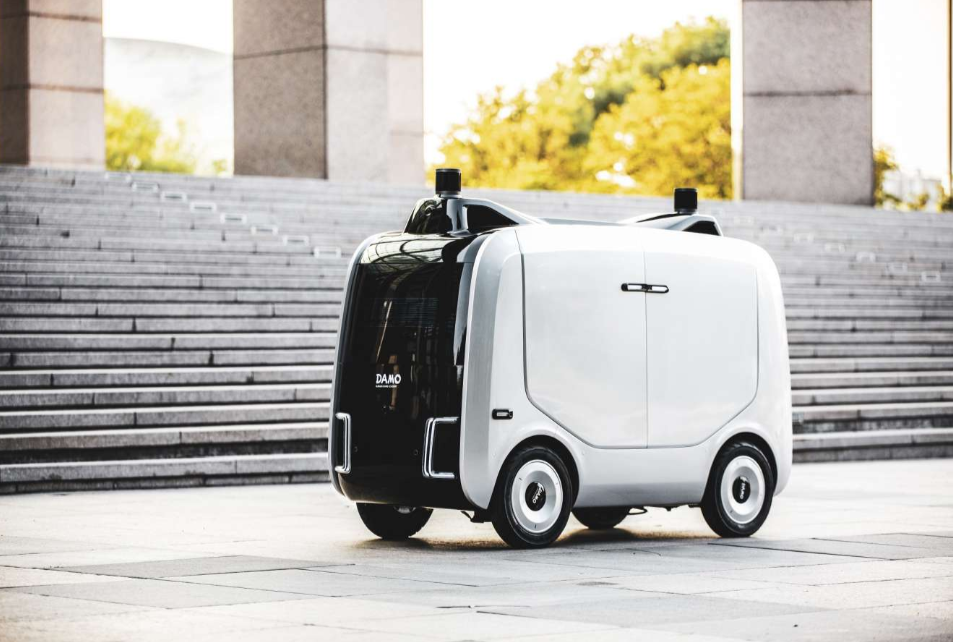
\includegraphics[width=0.55\textwidth]{delivery.png}
\caption{Example of an autonomous parcel delivery \cite{simonite2017hungry}}
\label{fig:delivery}
\end{figure}


\subsection{Industrial Units}
The robot is capable of moving tools, components and materials between work stations in factory floors. This minimises the amount of manual operation and accelerates the production. The system promotes the principles of automation and lean manufacturing. It also enhances safety because there is minimization of unnecessary human movement in hazardous areas.

\subsection{Hotels}
In hotels, the system can deliver room service items, laundry, and guest amenities. This enhances guest experience by providing fast and contactless service. The robot operates quietly in hallways and common areas. It also helps reduce staff workload during peak hours.

\subsection{Emergency and Disaster Zones}
In hazardous indoor environments, the robot can deliver essential supplies where human access is risky. It supports rescue operations by carrying tools, food, or medical kits. The system improves safety by reducing human exposure to dangerous conditions. Autonomous navigation ensures reliable operation in unstable environments.


\section{Limitations of the System}

Although the proposed system offers numerous advantages, it has certain limitations. The robot’s performance depends on sensor accuracy, battery capacity, and environmental conditions. The system is designed for flat indoor surfaces and may not perform effectively on stairs or uneven terrain. Network connectivity issues may affect real-time monitoring. These limitations provide direction for future improvements.

\section{Project Plan}
The following table shows the proposed project plan and timeline. The entire project, spanning literature review, algorithm development, web interface implementation, and full ROS 2/Gazebo simulation integration, was successfully completed within a total duration of \textbf{32 weeks}.

\begin{table}[H]
	\centering
	\caption{Proposed Project Plan and Timeline}
	\label{tab:project_plan}
	\begin{tabular}{|c|p{6cm}|c|p{5cm}|}
		\hline
		\textbf{S\#} & \textbf{Tasks} & \textbf{Duration} & \textbf{Resource Person} \\
		\hline
		1 & Literature Review & 02 Weeks & M.Ali, Aitzaz Arshad, Gulfam Haider \\
		\hline
		2 & Path Planning (A*/IA*) + Pruning & 02 Weeks & M.Ali, Aitzaz Arshad, Gulfam Haider \\
		\hline
		3 & Path Smoothing (PSO + Cubic Spline) & 02 Weeks & M.Ali, Aitzaz Arshad \\
		\hline
		4 & Model Predictive Control (MPC) Design \& Implementation & 02 Weeks & Aitzaz Arshad, Gulfam Haider \\
		\hline
		5 & Cellular Decomposition \& Dynamic Programming Integration & 02 Weeks & M.Ali, Aitzaz Arshad, Gulfam Haider \\
		\hline
		6 & Web Interface -- Frontend Development (Flutter) & 03 Weeks & M.Ali, Aitzaz Arshad \\
		\hline
		7 & Web Interface -- Backend Development (Flask) \& API Integration & 04 Weeks & M.Ali, Aitzaz Arshad \\
		\hline
		8 & ROS 2 Jazzy Installation \& Virtual Environment Configuration & 01 Week & M.Ali, Aitzaz Arshad, Gulfam Haider \\
		\hline
		9 & Gazebo Simulation World Design (Multi-Room Delivery Environment) & 02 Weeks & M.Ali, Aitzaz Arshad, Gulfam Haider \\
		\hline
		10 & SLAM Implementation \& Occupancy Grid Mapping & 01 Week & M.Ali, Aitzaz Arshad, Gulfam Haider \\
		\hline
		11 & Porting Path Planning, Smoothing \& MPC Algorithms into ROS 2/Gazebo Simulation & 03 Weeks & M.Ali, Aitzaz Arshad, Gulfam Haider \\
		\hline
		12 & Web -- Gazebo -- ROS 2 Full System Integration & 03 Weeks & M.Ali, Aitzaz Arshad \\
		\hline
		13 & System Testing \& Performance Evaluation & 02 Weeks & Aitzaz Arshad, Gulfam Haider \\
		\hline
		14 & Documentation \& Final Report Writing & 03 Weeks & M.Ali, Aitzaz Arshad, Gulfam Haider \\
		\hline
	\end{tabular}
\end{table}

\section{Project Timeline}
The following figure shows the Gantt chart for the project schedule, covering the complete 32-week duration of the project.
\begin{figure}[H]
	\centering
	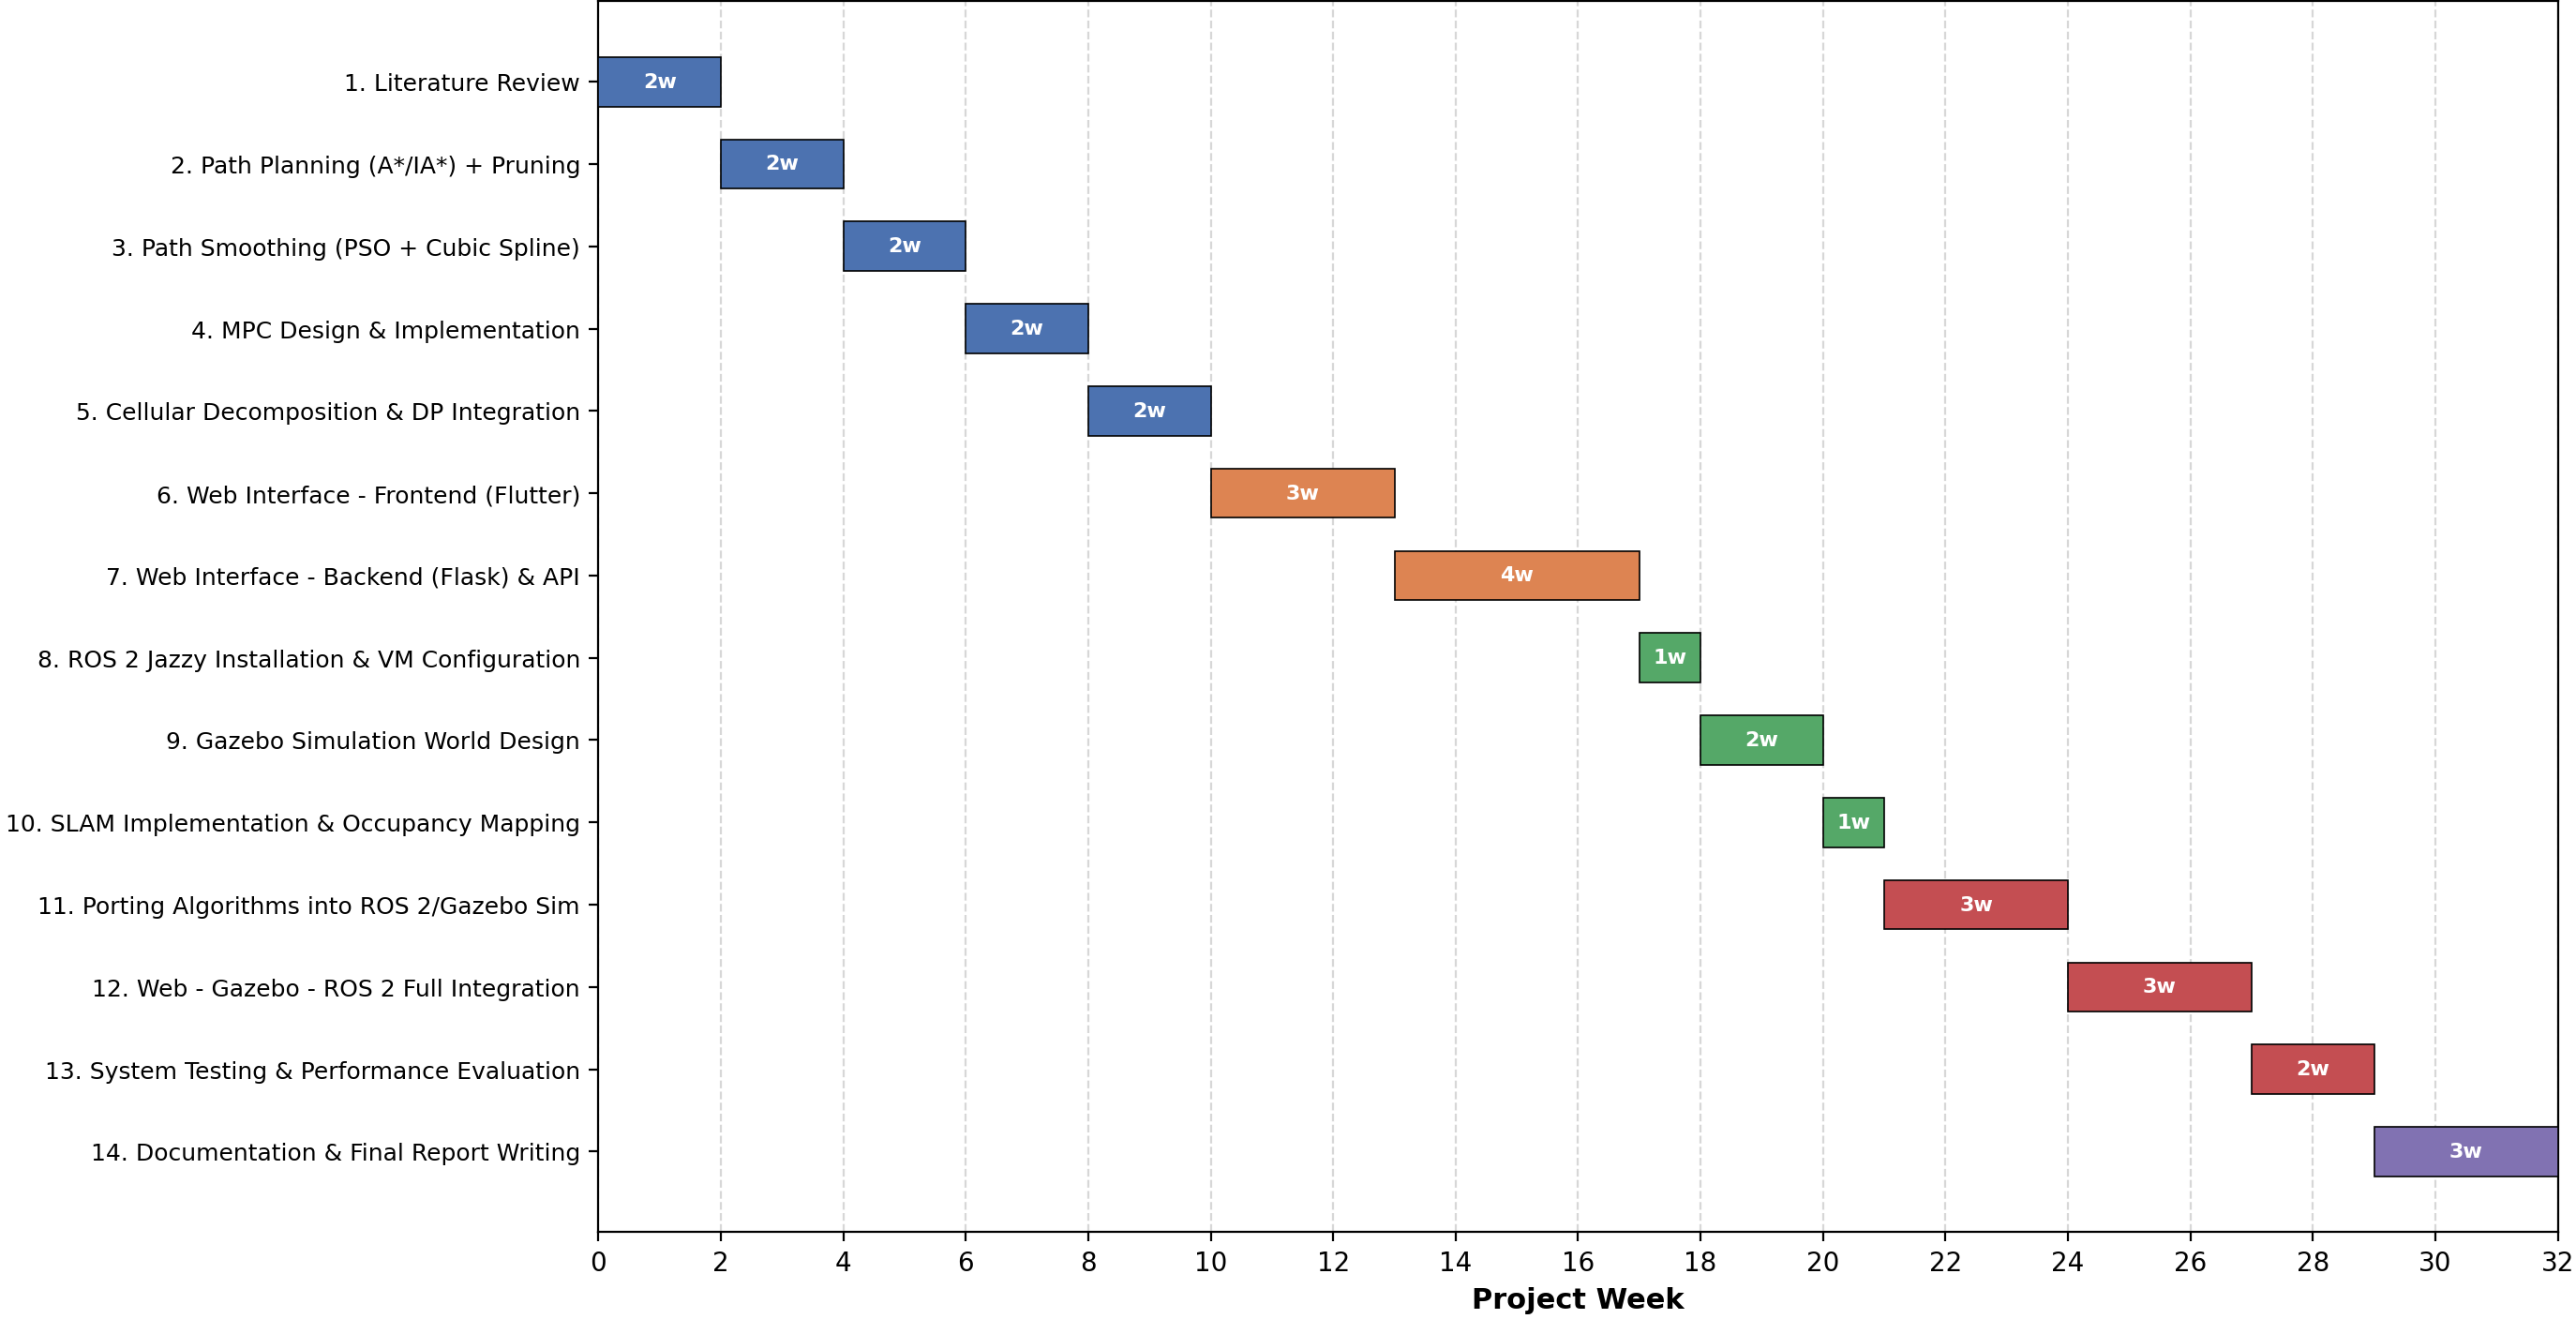
\includegraphics[width=1.0\textwidth]{chart.png}
	\caption{Project Timeline (Gantt Chart)}
	\label{fig:gantt_chart}
\end{figure}

\subsection{Targeted Sustainable Development Goals}

This project aligns with the United Nations Sustainable Development Goals (SDGs) by addressing key challenges in healthcare logistics, education, infrastructure innovation, and sustainable community living. The specific SDGs targeted by the Autonomous Parcel Delivery System are detailed in Table \ref{tab:sdgs}.

\begin{table}[h]
\centering
\caption{List of Targeted Sustainable Development Goals}
\label{tab:sdgs}
\renewcommand{\arraystretch}{1.5} % Adds vertical padding for better readability
\begin{tabular}{|c|p{0.25\textwidth}|c|p{0.45\textwidth}|}
\hline
\textbf{S\#} & \textbf{Targeted SDGs} & \textbf{SDG No.} & \textbf{Implementation Detail} \\ \hline
1 & Good Health and Well-Being & SDG \#3 & 
Autonomously transports medical supplies and lab reports in hospitals, reducing staff workload and minimizing human contact to lower cross-contamination risks. \\ \hline
2 & Quality Education & SDG \#4 & 
Supports academic operations on university campuses by efficiently delivering documents, assignments, and equipment between faculty offices, libraries, and laboratories. \\ \hline
3 & Industry, Innovation, and Infrastructure & SDG \#9 & 
Develops a scalable autonomous delivery architecture using ROS~2 to modernize internal logistics in warehouses and commercial buildings. \\ \hline
4 & Sustainable Cities and Communities & SDG \#11 & 
Promotes smart community living in universities and offices by reducing congestion and improving operational efficiency through automated delivery. \\ \hline
\end{tabular}
\end{table}\section{Report Organization}
The report is structured to provide a clear understanding of the project from background to results. Chapter 1 introduces the project, including its motivation, objectives, specifications, and scope. Chapter 2 reviews existing literature on path planning algorithms, mobile robot control strategies, ROS 2 navigation architecture, and previous implementations, highlighting gaps in current approaches. Chapter 3 explains the design and implementation of the custom navigation system, covering the IA* path planning algorithm, path smoothing methods, motion controller design, and ROS 2 integration. Chapter 4 describes the tools and techniques used, including the TurtleBot3 hardware, ROS 2 framework, Gazebo simulation, Python programming, and RViz visualization. Chapter 5 presents project results and evaluation, discussing navigation performance, tracking accuracy, path quality, web interface and Ros.Chapter 6 provides the conclusion and future work, summarizing achievements, lessons learned, limitations, and recommendations for enhancements like dynamic obstacle handling, multi-robot coordination, and real-world deployment. Chapter 7 relates the project to Sustainable Development Goals (SDGs), showing how autonomous navigation contributes to innovation, sustainable cities, and responsible production. Finally, Chapter 7 provides the conclusion and future work, summarizing achievements, lessons learned, limitations, and recommendations for enhancements like dynamic obstacle handling, multi-robot coordination, and real-world deployment.

\section{Chapter Summary}

This chapter provided a comprehensive introduction to the user-friendly autonomous parcel delivery system. It discussed the background, motivation, problem statement, proposed solution, objectives, scope, significance, applications, limitations, and project milestones. The chapter establishes a strong foundation for the technical and analytical discussions presented in the subsequent chapters.
	\chapter{LITERATURE REVIEW}
The issue of mobile robot navigation is something that a lot of people in schools are looking at. People are still trying to figure out how to make it better. They are working on things like figuring out where the robot is seeing what is around it planning a path and making it move. This part of the book looks really closely at the ideas and technologies that make indoor parcel-delivery systems work.New navigation systems are really good at making maps of the area and finding things that're in the way. They can also plan a path that's safe and works well. These systems use platforms like ROS 2 that help all the parts talk to each other.Also because of advances, in computer vision, deep learning and simulated environments autonomous robots are becoming more reliable and easier to use. Autonomous mobile robot navigation is getting better because of these things. Autonomous mobile robot navigation systems are being used in places now.
\section{Background}


The ideas talked about in this paper are the plan for the idea and actual creation of autonomous indoor delivery robots. To design systems we need to really understand how navigation works, how to figure out where the robot is, how to plan its path how to control its movement and how to put all the parts together. The following ideas are what tell us how to make the autonomous delivery robot work, in the world they help us decide which algorithms, sensor packages and software architectures to use to make autonomous indoor delivery robots work well.

Mobile robot navigation fundamentally depends on understanding the kinematic constraints of the robot platform. Differential drive robots, such as the TurtleBot3, operate under nonholonomic kinematic constraints, meaning they cannot move freely in all directions at a single instant. Instead, their motion is restricted to movements that are physically achievable through wheel rotations.

In differential-drive robots, we essentially drive the movements of two wheels on (one on each side of) the chassis that are driven independently by two motors. That is because the coordinated actuation of said wheels determines the linear velocity of the robot v and the angular velocity of the robot, which is 0. These input commands have a direct impact on the pose of the robot, its position and orientation in a global frame. The kinematic correlation between the inputs of the velocity and the change of pose is given as:

\begin{equation}
\begin{bmatrix}
\dot{x} \\
\dot{y} \\
\dot{\theta}
\end{bmatrix}
=
\begin{bmatrix}
v \cos(\theta) \\
v \sin(\theta) \\
\omega
\end{bmatrix}
\end{equation}

where:
\begin{itemize}[noitemsep]
\item $x, y$ represent the robot's position in the global coordinate frame
\item $\theta$ represents the robot's heading angle (orientation)
\item $\dot{x}, \dot{y}$ represent linear velocity components along the x and y axes
\item $v$ represents linear velocity
\item $\omega$ represents angular velocity
\end{itemize}

These kinematic constraints limit the robot's ability to execute arbitrary motion trajectories. Consequently, real world navigation needs to smooth path, plan trajectory and offer proper motion control measures to have viable and steady movement of a robot.

\subsection{Autonomous Mobile Robot Navigation Fundamentals}



The idea of autonomous mobile robot navigation is to allow robots to navigate in a safe and efficient way in a given environment. There are generally localization, mapping, path planning, obstacle avoidance, and motion control aspects of the navigation systems. These modules enable robots to know their locations, learn about the surrounding structures, design collision-free fields of movement and implement movement directions. Indoor delivery robotic systems are built on the incorporation of these elements of navigation within warehouses, hospitals, and academic institutions.
\subsection{Trajectory Smoothing and Interpolation}

Raw paths from planning algorithms like grid-based or sampling-based planners often have turns.These paths also have curvature and are not feasible for robots with kinematic constraints.The sharp turns and discontinuous curvature cause difficulties for differential drive robots.These robots need to follow motion profiles and meet their nonholonomic constraints.Differential drive robots have trouble, with paths that have turns.Their motion profiles must be smooth and continuous.They also have to comply with their constraints.. To overcome these constraints, they use trajectory smoothing to turn discrete paths represented as waypoints into continuous and differentiable paths with the use of waypoints as prongs of a path representation ~\cite{ravankar2018path}. This process is based on the technique of interpolation methods to produce smooth curves that must satisfy the velocity conditions, deceleration conditions and curvature conditions necessary to obtain stable robotic movement. When the sudden directional changes due to the trajectory smoothing are removed, the tracking accuracy would be improved, the mechanical forces acting on the actuators would be reduced, and the efficiency of the whole-navigation system would be raised.  

These methods that use spline interpolations are very useful for smoothing trajectories, as are interpolation methods. This is because spline interpolations are very flexible and are mathematically meaningful. There are a types of spline interpolations but the most common ones are cubic splines and B-splines.Cubic splines are good because they make curves that're smooth and have no sharp turns. They ensure that the position, velocity and acceleration of each section of the curve are the same. This means that cubic splines can follow the set of waypoints for which we are given and the transitions between them are smooth.The cubic splines and B-splines are important, for interpolation methods based on spline interpolations. B-splines have the opposite characteristics, however, because they are not strictly interpolated but only approximated the waypoints. The nature of this gives B-splines the ability to generate more smooth trajectories with finite curvature which is particularly useful in mobile robot motion tracking when using motion tracking controllers. The generated trajectory is dynamically realistic and can be synthesised by control algorithms, and can be used by differential-drive robots to follow predetermined trajectories safely and efficiently, due to the use of spline-based smoothing to ensure the trajectory is dynamically realistic.

\textbf{Natural Cubic Spline Interpolation for Path Smoothing}

Mobile robots require a smoothing algorithm for navigation, since many algorithms like A* and RRT produce piecewise-linear paths with abrupt changes in direction. Such non-circular motions are in contradiction to the kinematic constraints of differential-drive robots, which leads to jerky motions, loss of tracking accuracy and mechanical fatigue. The discrete sequence of waypoints is converted to a continuous curve by trajectory smoothing methods, that are kinematically allowed, yet are continuous and differentiable, and could be actually executed by a robot by using continuously differentiable curves.

The natural cubic splines are very popular as an interpolation method in robotics, due to their smoothness and ease of computation, as well as the fact that they are naturally easy to interpolate. A natural cubic spline is a discontinuous cubic polynomial that passes through each one of the given waypoints and is continuous at both the first and second derivatives at all of the continuity points.

These derivative conditions ensure that the resulting trajectory has smooth velocity and acceleration profiles which are essential in the realization of stable and compliant motion control.
\textbf{Mathematical Definition of Natural Cubic Splines}
The mathematical expression of natural cubic splines is in line with standard numerical 
analysis approaches~\cite{siciliano2016springer}.
Given a sequence of n + 1 waypoints $(x_0, y_0), (x_1, y_1), \ldots, (x_n, y_n)$, a natural cubic spline $S(t)$ consists of n cubic polynomial segments:

\begin{equation}
S_i(t) = a_i + b_i(t - t_i) + c_i(t - t_i)^2 + d_i(t - t_i)^3, \quad t \in [t_i, t_{i+1}]
\end{equation}

where $i = 0, 1, \ldots, n - 1$, and $t$ is a parameter (typically arc length or normalized distance).

The spline coefficients $(a_i, b_i, c_i, d_i)$ are determined by enforcing the following constraints:

\begin{enumerate}[noitemsep]
\item \textbf{Interpolation:} The spline passes through all waypoints:
\begin{align}
S_i(t_i) &= y_i \quad \text{and} \quad S_i(t_{i+1}) = y_{i+1}
\end{align}

The spline coefficients $(a_i, b_i, c_i, d_i)$ are obtained by satisfying the following conditions:
\begin{equation}
S_i'(t_{i+1}) = S_{i+1}'(t_{i+1}), \quad i = 0, 1, \ldots, n - 2
\end{equation}

\item \textbf{$C^2$ Continuity:} Second derivatives at the end points are zero:
\begin{equation}
S_i''(t_{i+1}) = S_{i+1}''(t_{i+1}), \quad i = 0, 1, \ldots, n - 2
\end{equation}

\item \textbf{Natural Boundary Conditions:} Second derivatives at the endpoints are zero:
\begin{equation}
S_0''(t_0) = 0 \quad \text{and} \quad S_{n-1}''(t_n) = 0
\end{equation}
\end{enumerate}

These restrictions give rise to a tridiagonal matrix system of $(n+1)$ linear equations, which can be solved efficiently via tridiagonal matrix methods. The natural boundary condition guarantees that the curve that is obtained is the ``smoothest'' possible interpolation that minimizes the total curvature energy.

\textbf{Parametric Representation for Robot Path Planning}
The standard $y = f(x)$ form is not used for mobile robot trajectories in 2D space; instead, a parameterization is used. Both x and y coordinates are functions of a parameter $t$ in parametric form:

\begin{equation}
P(t) = \begin{bmatrix} x(t) \\ y(t) \end{bmatrix}
\end{equation}

where \(x(t)\) and \(y(t)\) represent natural cubic splines that are independently fitted to the \(x\)- and \(y\)-coordinates of the waypoints, respectively.

\textbf{Why Parametric Representation?}

\begin{itemize}[noitemsep]
\item \textbf{Handles Vertical Segments:} Unlike standard splines, which require monotonically increasing \(x\)-values and therefore cannot accurately represent vertical or looping paths, parametric splines eliminate this limitation by treating both coordinates as functions of a common parameter.
\end{itemize}

\subsection{Localization and Mapping Principles}

Accurate localization and environmental mapping are essential for reliable robot navigation.Simultaneous localization and mapping, also known as SLAM, represent an important category of methods that enables robotic systems to build detailed maps of the previously unknown space and also determine their own location on the map. These types of SLAM utilize large collections of sensors to collect high-fidelity environmental data such as visual cameras, laser scanning systems (LiDAR) and inertial measurement systems (IMU). Combining these sensory signals, the mappings do not only enable the detection of obstacles and the recognition of landmarks in the navigation process, but also provide the basis of designing strong and effective path-planning algorithms.
\subsection{Path Planning and Obstacle Avoidance Fundamentals}

	Path planning focuses on generating optimal and collision-free trajectories between start and destination points.Simultaneous localization and mapping, also known as SLAM, represent an important category of methods that enables robotic systems to build detailed maps of the previously unknown space and also determine their own location on the map. These types of SLAM utilize large collections of sensors to collect high-fidelity environmental data such as visual cameras, laser scanning systems (LiDAR) and inertial measurement systems (IMU). Combining these sensory signals, the mappings do not only enable the detection of obstacles and the recognition of landmarks in the navigation process, but also provide the basis of designing strong and effective path-planning algorithms.

\subsection{Motion Control and Trajectory Tracking}

Motion control strategies help robots follow planned paths and move smoothly. They do this while staying stable.Traditional control methods, like Proportional-Integral-Derivative regulators are widely used to control the speed of motors and follow set paths.Advanced methods, Model Predictive Control work better for navigation. Model Predictive Control does this because it can predict what the robot will do in the future and control its movements to work best with the situation and any limitations of the robot and its environment.Model Predictive Control is a type of motion control strategy that helps robots navigate.
\subsection{Robotics Middleware and System Integration}

\begin{sloppypar}
	Robotic middleware platforms provide communication and integration frameworks that connect perception, navigation, and control modules. As it has been mentioned, the Robot Operating System 2.0 offers a modular architecture, the real-time facilitation of communication, and scalability, thus supporting autonomous robotic platforms. ROS2 enables the easy addition of perception algorithms, navigation stacks, simulation systems and user-interface systems, thus facilitating the development of complex autonomous delivery systems.
\end{sloppypar}

\section{Related Technologies}

Path planning is one of the problems in autonomous mobile robotics. Find a route from a start location to a target location without hitting anything in the way. This walk should be efficient as well. The path planner is extremely crucial as it impacts on the safety of the navigation, the smoothness of all the processes and the efficiency of time. Lots of algorithms have been proposed. Each one has its good and bad points like how good the path is, how much it costs to compute and how well it works in environments that are changing.In this section we will look at new path planning algorithms. We will also go though the reason for selecting the Improved A* algorithm for this project.

\subsection{Related Technology 1 -- Path Planning Algorithms}
Path planning is an issue in autonomous mobile robotics. We need to find a path, from a start location to a target without hitting anything. This path also needs to be efficient. The path planner is really important because it affects how safe the navigation is, how smooth everything runs and how well it works in time. There are a lot of algorithms that people have suggested. Each one has its good and bad points like how good the path is, how much it costs to compute and how well it works in environments that are changing.In this section we will look at new path planning algorithms. We will also explain why we chose the Improved A* algorithm for this project. The Improved A* algorithm is what we picked for this project.

\subsubsection{A* Algorithm}

The A* algorithm is a widely used graph-based search method~ that finds the shortest path on a discretised map using the evaluation function:

\begin{equation}
f(n) = g(n) + h(n)
\end{equation}

where $g(n)$ is the accumulated cost from the start node to node $n$, and $h(n)$ is a heuristic estimate of the remaining cost from $n$ to the goal. When the heuristic is admissible (i.e., it never overestimates the true cost), A* guarantees an optimal solution. In indoor grid maps, Euclidean or Manhattan distance heuristics are typically employed\cite{zhang2022improved}.

The path finding method A* is very good at finding the path, but it creates a path with a lot of sharp turns which a robot can not follow. These robots have wheels that don't allow them to make these sharp turns easily. However, the route that A* has discovered is not adequate to use it away. The A* path needs to be fixed and made better before we can use it on a robot or a robot, in a simulation.

\subsubsection{Improved A* (IA*) Algorithm}

IA* is an extension of the A* algorithm, which introduces three key improvements for robotic navigation in such environments~\cite{wang2021mobile}:
\begin{itemize}
\item Diagonal Motion Support -- Enables movement in eight directions instead of four, resulting in shorter and more geometrically natural paths on occupancy grid maps.
\item Obstacle Inflation -- Obstacles are virtually enlarged by a safety margin, which is defined in the robot's planning, thus providing a clear margin of safety for the robot while navigating walls and physical obstacles.
\item Waypoint Pruning -- Line-of-sight checks are performed between non-adjacent nodes to remove unnecessary intermediate waypoints, resulting in a shorter and cleaner waypoint sequence that significantly reduces the computational effort required in the subsequent processing stages.
\end{itemize}

\subsubsection{Comparison with Other Path Planning Algorithms}

Table~\ref{tab:path_planning_comparison} compares IA* with planners.They check things like
These things are important, for delivery robots.The planners are judged on these criteria.IA* and other planners are compared.
\begin{table}[htbp]
\centering
\small
\caption{Comparison of Path Planning Algorithms}
\label{tab:path_planning_comparison}
\begin{tabular}{|p{2cm}|p{1.6cm}|p{1.6cm}|p{1.6cm}|p{2cm}|p{3cm}|}
\hline
Algorithm & Type & Complete & Dynamic & Path Quality & Key Limitation \\
\hline
Dijkstra & Graph & Yes & No & Jagged & Very slow on large maps \\
\hline
A* & Graph & Yes & No & Jagged & Needs smoothing \\
\hline
Improved A* (IA*) & Graph & Yes & Partial & Pruned & Requires smoothing \\
\hline
RRT & Sampling & Prob. & Yes & Irregular & Random, jagged paths \\
\hline
RRT* & Sampling & Prob. & Yes & Moderate & High computation cost \\
\hline
D* Lite & Graph & Yes & Yes & Jagged & Complex to implement \\
\hline
Potential Field & Reactive & No & Yes & Smooth & Local minima traps \\
\hline
\end{tabular}
\end{table}

\subsubsection{Justification for Selecting Improved A*}

From the comparison shown on Table~\ref{tab:path_planning_comparison}, the Improved A* algorithm was selected to be the global path planner for this project. The reasons for this are: Dijkstras algorithm explores all the nodes which is time intensive on large indoor maps, and Standard A* would give jagged output, which would be a lot of work with grid.It also does not have safety margins. Other planners such as RRT and RRT* were not selected as they are expensive to compute, and do not guarantee the paths that they generate.These planners may not be appropriate for 2D indoor spaces, such as ours.The use of Improved A* algorithm was chosen as the global path planner, as D* Lite would add unnecessary complexity of implementation as dynamic obstacle avoidance is handled in the local planner using real time sensor data. Local minima traps in corridor-based layouts are a known issue of Potential Field methods, which is why they were rejected.

The proposed system has all the key requirements covered by IA*: it works directly on the SLAM-generated occupancy grid map, ensures a near-optimal collision-free path, implements safety clearance by inflating obstacles and generates a compact pruned waypoint set that fits into the cubic spline smoothing and Model Predictive Control pipeline outlined in the next sections.

\subsection{Related Technology 2 -- Path Smoothing and Optimization Techniques}

\subsubsection{Overview}

Path smoothing is an important post-processing task for mobile robots navigating in real environments from piecewise-linear paths produced by discrete planners (e.g. A*, RRT). There are many smoothing methods available in the literature but in this section, we discuss two of them and consider the natural cubic spline method used in this project to put those methods into perspective.

\subsubsection{Classical Interpolation Approaches}

Cubic Spline Interpolation: We talked about this in Section 2.1.3. Cubic Spline Interpolation is a way to make smooth paths. It is used a lot in robotics because it works well and is smooth. The problem with Cubic Spline Interpolation is that it does not try to make the path as short as possible or make it very curvy. It just makes a path that goes through the points we give it.
B-Spline Approximation: B-Spline Approximation is different from Cubic Spline Interpolation. Of making a path that goes through all the points B-Spline Approximation makes a path that is close, to the points. We can control the shape of the path by moving some points.. This means that the path might not go through all the points we want it to. This can cause problems when we are trying to avoid things in the way. B-Spline Approximation is used more in computer aided design and making paths not so much in robotics where we need to go through specific points.~\cite{ravankar2018path,mercy2017spline}

\subsubsection{Optimization-Based Smoothing: PSO with Bezier Curves}

There have been recent studies on using Particle Swarm Optimization (PSO) and Bezier curves to create smooth optimized paths~\cite{song2020smooth}. This method considers path smoothing as an optimization problem, with the location of the points of the Bezier curves being the variables to be optimized.
\textbf{How it Works:}

\begin{enumerate}[noitemsep]
\item The positions of the interior control points are optimized by using PSO.
\item The positions of the interior control points are optimized by using PSO.
\item The fitness function minimizes:
\begin{itemize}[noitemsep]
\item Total path length
\item Maximum curvature
\item Curvature derivative (jerk)
\item Collisions with obstacles earn penalties (the distance between the object and obstacles).
\end{itemize}
\end{enumerate}

This produces a Bezier curve that is smooth and optimised and is guaranteed to have high order continuity.

\textbf{Advantages:}

\begin{itemize}[noitemsep]
\item Direct optimization of path length and path curvature bounds is possible with explicit optimization.
\item The $G^3$-continuity is naturally achieved by high degree Bezier curves with no further requirements.
\item PSO is a derivative-free method, which is suitable for non-convex optimization landscape with obstacle constraints.

\end{itemize}

\textbf{Disadvantages:}

\begin{itemize}[noitemsep]
\item \textbf{Computational Cost:} PSO needs to be evaluated iteratively (usually 50–100 particles evaluated in 20–50 iterations), which does not allow it to be used for real-time replanning.

\item \textbf{Parameter Sensitivity:} The PSO parameters (inertia weight, cognitive/social coefficients) play a crucial role in performance.

\item \textbf{No Interpolation Guarantee:} The optimized Bezier curve can have a huge deviation from the original A* waypoints in complex environments, and it might not clear obstacles.

\item \textbf{Convergence Uncertainty:} PSO is a stochastic algorithm and does not ensure global optimality and may have different results on different runs.
\end{itemize}

\subsubsection{Hybrid Approaches: Local PSO Optimization with Spline Smoothing}

The complementary strengths of both interpolation and optimization methods are acknowledged and considered, therefore, this project takes a hybrid approach of:

\begin{enumerate}[noitemsep]
\item \textbf{Global Path Planning:} Global Path Planning is achieved by improved A* which generates a collision-free waypoint sequence.
\item \textbf{Waypoint Pruning:} Line-of-sight checks eliminate unnecessary intermediate waypoints.
\item \textbf{Local PSO Refinement (Optional):}  In selected waypoints with tight corridors, it is possible to optimize their position within a small radius so that the curvature is minimized in the area without losing the obstacle clearance.
\item \textbf{Natural Cubic Spline Smoothing:} The pruned waypoint sequence is then smoothed using parametric cubic splines to generate the final executable trajectory.
\end{enumerate}

Hybrid means it will be a mix of spline interpolation and also improvements where needed. This method is always physically feasible, regardless of the use of the Particle Swarm Optimization refinement, thanks to spline smoothing. This involves a spline smoothing step, which is always performed and when used, always yields an acceptable result.

\subsubsection{Justification for Cubic Spline Selection}

Due to the following reasons, natural cubic splines were chosen for the autonomous parcel delivery application over PSO-Bezier optimization:

\begin{itemize}[noitemsep]
\item \textbf{Real-Time Performance:} The delivery robots in the indoor environment need to rapidly replan if there are obstacles. Deterministic and fast smoothing for dynamic environments is cubic splines.

\item \textbf{Obstacle Avoidance Guarantee:} Cubic splines interpolate through A* waypoints, thus maintaining the collision-free properties of the global planner. There can be deviations due to Bezier optimization that may need further validation.

\item \textbf{Integration with MPC:} Cubic splines can be easily combined with the Model Predictive Control representation and analytical derivatives for accurate trajectory tracking.

\item \textbf{Implementation Simplicity:} Using scipy.interpolate.CubicSpline is less complex to implement than implementing and tuning a PSO-Bezier optimizer, and more maintainable.
\end{itemize}

\subsection{Related Technology 3 -- Particle Swarm Optimization (PSO) Based Path Planning}

The Particle Swarm Optimization (PSO) is an evolutionary optimization algorithm that is based on population which finds numerous applications in robotics and autonomous navigation in finding solutions to nonlinear complex optimization problems~\cite{krell2019collision}. PSO has been applied for solving the smooth path planning problem of mobile robots, where a set of control points of continuous high-degree Bézier curves is optimized.

The article constitutes robot path planning as an optimization problem with several objectives like minimization of the path length, obstacle avoidance, a smooth curvature, and motion continuity being addressed together. The authors point out that traditional path planning methods tend to produce piecewise linear or polygonal-shaped paths that have sharp turns. These disjunctions lead to the result of frequent changing of motion states leading to unstable robot motion, high energy consumption as well as mechanical stress.~\cite{song2020smooth}.

In order to solve these problems we have an better PSO algorithm. This algorithm uses a kind of velocity update equation that changes over time.In the PSO algorithm we use the best solution found by each particle and the best solution found by all particles to update the position and velocity of each particle.Our new PSO algorithm also uses the particles velocity, which helps it search more widely and avoids getting stuck too early.
The new velocity update model is shown as:

\begin{equation}
v_i^{k+1} = w \cdot v_i^k + c_1 \cdot r_1 \cdot (p_{\text{best},i} - x_i^k) + c_2 \cdot r_2 \cdot (g_{\text{best}} - x_i^k) + \alpha \sum_{j=1}^{m} \beta_j v_i^{k-j}
\end{equation}

When particles move around their movement is affected by how they are going right now and also by how fast they were going before. This memory of what happened helps particles get out of tight spots and look around more.

The goal of the optimization is to make the path as short, as possible with not many sharp turns and the turns should be smooth too:

\begin{equation}
J = w_1 L + w_2 \int \kappa^2 ds + w_3 \int \left(\frac{d\kappa}{ds}\right)^2 ds
\end{equation}

This formulation ensures generation of smooth and dynamically feasible robot paths.

\subsubsection{Relevance to Our Project}

The PSO-based optimization system is very applicable to our mobile robot path planning project. Our project aims at the creation of collision-free smooth navigation paths through smart and intelligent planning algorithms that are incorporated into a web-based planner system.

The enhanced PSO method assists in optimization of smoothness of the path that is in direct relation with the path refinement and smoothing modules of our project. Moreover, the idea of addressing the path parameters optimization rather than the post-processing smoothing is used to complement our spline and smoothing solutions in the backend processing. Optimization based planning also contributes to dynamic adaptability important in real time generation and visualization of web based paths.

\subsubsection{Limitations Identified}

Although the enhanced PSO algorithm is efficient, a number of limitations exist. Additional computational complexity is also presented in the algorithm with the calculation of fractions-order velocity and adaptive parameter adjustment. This adds to the time of execution and it can reduce real-time performance in large or highly dynamic environments.

The approach also presupposes grid-like workspace, which is easier to represent obstacles with, but less applicable to irregular or unstructured setting. In addition, performance of optimization is also dependent on the choice of parameters like inertia weights and acceleration coefficients, which could need manual optimization according to the environment.

The other weakness is that the methodology is only tested based on simulation experiments instead of real robotic implementation. There is no discussion of practical implementation issues like noise of sensors, dynamic movement of obstacles and uncertainty in localization.


\subsection{Related Technology 4 -- Motion Control Strategies for Trajectory Tracking}

Trajectory-tracking controllers compute velocity commands required to follow a reference trajectory while minimizing tracking error and satisfying kinematic constraints. Approaches to trajectory tracking range from model-based predictive optimization to learning-based strategies.

\subsubsection{Model Predictive Control (MPC)}

MPC optimizes control inputs over a finite prediction horizon by solving a constrained optimization problem at each timestep~\cite{faulwasser2009mpc}. Using a point-mass dynamics abstraction based on double-integrator models derived from Newton's second law ($F = ma$), the discrete-time system can be represented as

\begin{equation}
	x_{k+1} = A x_k + B u_k
\end{equation}

where the state vector contains position and velocity, $x = [x, y, v_x, v_y]^T$, and the control input consists of accelerations, $u = [a_x, a_y]^T$. This point-mass abstraction simplifies the robot dynamics while preserving the essential relationship between path geometry and tracking performance, allowing the effect of curvature continuity on control stability to be analysed without requiring explicit differential-drive wheel kinematics. MPC aims to minimize the following cost function:

\begin{equation}
	J = \min_{U} \sum_{i=1}^{N_p} \left( e_i^T Q e_i + u_i^T R u_i \right)
\end{equation}

The tracking error, $e_i = x_i - x_{\text{ref},i}$, is penalized by $Q$; the tracking effort, $u_i$ or $y_i - x_{\text{ref},i}$, is penalized by $R$; and $N_p$ is the prediction horizon. Constraints like velocity limits and acceleration bounds are naturally imposed on MPC by convex optimization solvers, and when provided with smooth reference trajectories, MPC can prove more accurate at tracking them.

Very much the performance of the MPC depends on the smoothness of the reference path's. If the path is not smooth and has turns it can cause big problems, with the prediction model. This means the MPC will make mistakes and the control will keep changing back and forth. Studies have shown that using paths can make a huge difference it can reduce the tracking error by a really big amount compared to using piecewise-linear references. The MPC performance is much better when the reference path is smooth~\cite{cao2024pure}.

\subsubsection{Pure Pursuit Control}

Pure Pursuit~\cite{cao2024pure}The robot figures out how to move by finding the circular path between where it is now and a point a little ahead on the path it is supposed to follow. This way of doing things is easy to set up. It works well.. It also assumes that the robot will always be moving at the same speed, which can cause problems when the path has curves that are different, from each other. The robot has trouble following the path when it has to make turns that're not all the same.

\subsubsection{Deep Reinforcement Learning (DRL) for Path Following}

Recent research~\cite{cao2024pure} explores a way to control mobile robots. It uses a mix of Pure Pursuit steering and Soft Actor-Critic velocity control. This helps the robot adjust its speed based on the path it is taking.Some control methods that use Deep Reinforcement Learning can learn to behave in ways. They need a lot of practice in a fake environment first. It takes a considerable amount of practice in a fake environment before they can do this. They also are difficult to comprehend. May not be successful in new settings through additional practice.On the hand Model Predictive Control is good, at handling limits and making robots behave predictably.. It requires easy pathways for it to function properly.

\begin{table}[htbp]
	\centering
	\caption{Motion Control Technologies Relevant to This Project}
	\label{tab:motion_control_tech}
	\begin{tabular}{|p{3.2cm}|p{3.2cm}|p{6.6cm}|}
		\hline
		\textbf{Component} & \textbf{Tool/Method} & \textbf{Description} \\
		\hline
		Offline Control Analysis & Model Predictive Control (MPC) & Quadratic programming, point-mass dynamics, demonstrates curvature-tracking relationship \\
		\hline
		Constraint Handling & CVXPY (Quadratic Solver) & Velocity limits and acceleration bounds enforcement \\
		\hline
		Localization & AMCL (Particle Filter) & Monte Carlo localization, laser scan matching \\
		\hline
	\end{tabular}
\end{table}

\subsubsection{Relevance to Our Project}

MPC is compatible with our system. It relates the degree of smoothness of the anticipated trajectory with the ability of the system to follow and control the trajectory.What we've done is to do an analysis and it showed that it's better to use paths rather than using direct waypoints.That is why we make use of paths in the controller.It supports the delivery of parcels smoothly and evenly in standalone mode.The smoothed paths make sure that the system will follow the path and not miss any parts of it.This accurate following leads to movements, during parcel delivery.

\subsection{Related Technology 5 -- Cellular Decomposition}

One of the most common place planning techniques, called cellular decomposition, is used in autonomous robot navigation in classical environment representation~\cite{galceran2013survey}. The way divides the robot space into sections with no overlaps. These sections are called cells. This makes it easier to navigate because the open area is now organized.It is a method that makes computing more efficient. It also reduces crashes. Helps create paths in a systematic way.The cell structure helps robots move around without bumping into things. This way the robot can find its way more easily.Cells make navigation simpler. The robot area is split into cells. This helps with path creation.
Recent studies indicate that cellular decomposition is done by subdividing the free space into a finite number of smaller cells where:

\begin{equation}
W_{\text{free}} = \bigcup_{i=1}^{N} C_i
\end{equation}

where $C_i$ represents each decomposed navigable cell and $N$ is the total number of cells. Each cell is either free or occupied depending on if there is an obstacle in it. This way of breaking things down makes it easier to plan a path by moving through cells that are next, to each other instead of looking at the whole area.

Most new ways of doing things use a method called cellular decomposition, where each cell is a convex shape meaning it satisfies certain conditions that make it convex.~\cite{choset2001coverage}. Convex cells are very important as they ensure that you can draw a line between any two points within the cell without intersecting anything that may be present. The rule, for convex cells can be stated like this:
\begin{equation}
\forall p_1, p_2 \in C_i, \quad \lambda p_1 + (1-\lambda) p_2 \in C_i, \quad \lambda \in [0,1]
\end{equation}

This property greatly simplifies path planning. Enhances the ability to detect collisions.Cellular decomposition enables the construction of a graph which illustrates the connections between cells. Each cell is a node. Cells that are next to each other have lines between them on the graph.To find the path we look for the one that costs the least to travel between cells that are connected.The cost is usually based on things like distance or obstacles.The cost function, in cell-based planning is typically defined as:

\begin{equation}
J = \sum_{i=1}^{n-1} d(C_i, C_{i+1}) + n \cdot c_{\text{transition}}
\end{equation}

where $d(C_i, C_{i+1})$ represents the distance between adjacent cell centers and $n$ denotes the number of transitions between cells.
Cellular decomposition is a method that has been improved by research. This method is now used with techniques like Astar and dynamic programming. When we use these methods together we can find the path on a large scale. This is done by choosing the way to move from one cell to another. We also store the paths we have already calculated so that we can use them again and do not have to spend a lot of time calculating them.

Some new ways of using decomposition can change the size of the cells based on where the obstacles are. This helps the method work better and find the path.

Cellular decomposition can make complex places easier to navigate, in part. This is very useful if we are using robots within buildings. The cellular decomposition is also useful for avoiding obstacles for robots. We can easily use it with methods, like Particle Swarm Optimization and Model Predictive Control.

\textbf{Advantages of Cellular Decomposition}

\begin{itemize}
\item Breaks down complex environments to create a structure of navigation regions
\item Compresses computation time by using graph based path planning.
\item Enhances collision avoidance by using structured representation of obstacles
\end{itemize}

\subsubsection{Relevance with Our Project}
The cellular decomposition is directly related to the navigation system that we are talking about as this will give us a clear picture of the robots workspace. We have divided the space into grid cells to distinguish the free space from space with obstacles. This way of breaking down the space is also helpful when we are planning the path that the robot will take because we can use algorithms like A* and Dynamic Programming to search for a path, through the cells instead of having to search the whole space. The cellular decomposition also helps us to detect collisions make maps more efficiently in a web-based planner and find the best paths and track the movements of the robot using PSO and MPC in the ROS2-Gazebo simulation platform.

\subsubsection{Limitations of Cellular Decomposition}

\begin{itemize}
\item \textbf{High Computational Cost:} The finer the grid, the more memory will be used and the more complex the calculation.
\item \textbf{Resolution Dependency:} Small cells slow down processing speed and large cells decrease planning accuracy.
\item \textbf{Difficulty in Dynamic Environments:} There is a need for repeated decomposition and replanning due to frequent changes in the environment.
\item \textbf{Path Suboptimality:} Decomposition in the grid may result in longer or less smooth paths than continuous space planning methods.
\item \textbf{Scalability Issues:} Works poorly in large or complex spaces.
\end{itemize}

\subsection{Related Technology 6 -- ROS2-Based Autonomous Robot Architectures}

ROS is now an established middleware to create robotic applications. However it had some issues with scalability and real-time performance.This led to the creation of ROS2, which aims to meet the needs of autonomous robot development.Recent research on robotics reveals that many of the ROS2-based systems are dedicated to enhancing autonomy.They are the most advanced robots in the field.This Semester we will be learning about them.The newest reviews pertain to systems based on ROS2 to improve autonomy.This includes ROS2-based systems.Autonomy is an area of focus, for these systems.ROS2 is being used to improve autonomy.~\cite{bonci2023ros2}. The papers highlight modular designs where the perception, planning, and control are separated and ensure that the system can maintain scalability and flexibility without getting trapped in an inflexible design. In other works, the topic of practical designing and executing autonomous mobile robots in unstructured indoor settings is examined~\cite{gargouri2024cost}. These systems include hardware such as motors, sensors and controllers in addition to software modules in navigation and obstacle avoidance. Architectural and hardware-centric methods are both shown to be able to use ROS2 to support autonomous navigation. The comparison shows the usefulness of mixing ROS2 modular software stacks with practical hardware integration; this has been our first-hand experience, which we are applying to the design of our proposed autonomous parcel delivery system.

\subsubsection{Advantages and Limitations of ROS2-Based Systems}

ROS2-based autonomous systems offer several advantages:

\begin{itemize}
\item Modular and scalable architecture
\item Real-time communication support
\item Greater reliability and fault-tolerance.Better reliability and fault tolerance.
\item A strong community and ecosystem support base.
\end{itemize}

However, limitations include:

\begin{itemize}
\item Increased system complexity
\item Steeper learning curve
\item Hardware integration challenges
\item Computational cost on low-cost platforms
\end{itemize}

The trade-offs are recognized in both architectural and implementation studies, and the importance of balancing the design of the system involves complexity and performance issues.


\subsection{Related Technology 7 -- ROS2 Navigation Stack (NAV2 Framework)}

The ROS2 Navigation Stack, which is also known as NAV2 gives us a solution for autonomous robot navigation. NAV2 has a lot of parts including modules for localization, mapping, path planning and motion control. When it comes to localization we usually use something called Adaptive Monte Carlo Localization or AMCL for short to figure out where the robot is. This is done by using LiDAR data and a map that we already know.The ROS2 Navigation Stack or NAV2 also does mapping by using something called SLAM algorithms to make occupancy grid maps.NAV2 has path planning, which is split into two parts: planners that help the robot plan long routes and local planners that help the robot avoid things that are in its way.People who work on NAV2 whether they are in school or, in industry think it is very important to use data from sensors, LiDAR and IMU to make navigation work well. The ROS2 Navigation Stack or NAV2 is used to make sure the robot can move around safely.
\subsection{Related Technology 8 -- Visual SLAM vs LiDAR-Based SLAM}

SLAM systems are commonly categorized based on the primary sensor used for perception: visual sensors (cameras) or LiDAR sensors. Visual SLAM systems rely on monocular, stereo or RGB-D cameras to derive features and obtain depth data~\cite{campos2021orb}. They offer high appearance at low cost and are ideal in indoor environment conditions in which there are texture and lighting cues. However, they are sensitive to light effects and change of scene. In contrast, LiDAR-based SLAM is a process which employs laser scanners to create 3D point clouds, which do not depend on lighting conditions~\cite{li2021indoor}. LiDAR does not have, even though it is able to offer very accurate geometrical measurements. Recent deep learning-based visual SLAM prove that systems based on cameras can be accurate in the same way as LiDAR at the same time as they are cost-effective in hardware, which makes them ideal in indoor autonomous delivery robots.

\subsection{Related Technology 9 -- DROID-SLAM Framework and Dense Bundle Adjustment}

DROID-SLAM~\cite{teed2021droid} is a deep learning-based visual SLAM system that can be used with monocular, stereo, and RGB-D cameras. The system utilizes a recurrent neural architecture that does a sequential optimization of camera pose and dense depth maps. The use of Dense Bundle Adjustement (DBA) in a fully differentiable pipeline is another key innovation. Unlike the classical SLAM that performs sparse BA, DROID-SLAM performs joint optimization of pixel-wise depth and multiple camera poses. This repetition optimization does help a great deal to diminish drift and improves tracking strength which is particularly good in low-texture indoor places like walls and floors. Also, the framework makes generalizations across sensor modalities, without re-generalizing training. In the case of autonomous parcel delivery robots, the DROID-SLAM facilitates high levels of acculocalize rates with the help of a low-cost RGB or RGB-D camera alone.

\begin{figure}[htbp]
\centering
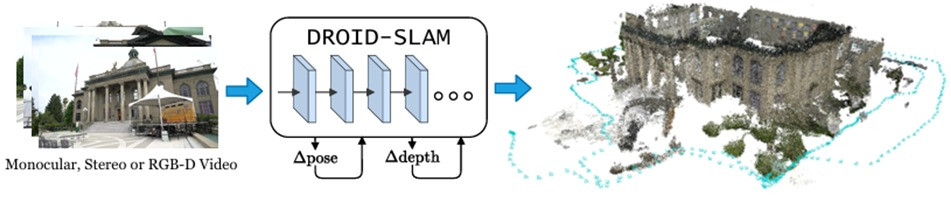
\includegraphics[width=0.8\textwidth]{droid.jpeg}
\caption{DROID-SLAM System Architecture~\cite{teed2021droid}}
\label{fig:droid_slam}
\end{figure}

\subsection{Related Technology 10 -- MAGiC-SLAM Multi-Agent Gaussian Mapping}

MAGiC-SLAM~\cite{yugay2024magic} introduces a multi-agent SLAM framework based on a 3D Gaussian scene representation. Rather than describing the environment as the point clouds or voxels, the model is represented by Gaussian primitives that enable the representation of the scene in an efficient manner, and map merging. The most important contribution of MAGiC-SLAM is that it is capable of fusing maps formed by several robots into a map on a global scale by the means of trajectory alignment and loop closure. This method enhances large indoor en-scalability, vironments and minimizes drift. In a place where numerous delivery robots are used at the same time, e.g. warehouses or hospitals, MAGiC-SLAM provides a viable tool of collaborative mapping and common space understanding.

\begin{figure}[htbp]
\centering
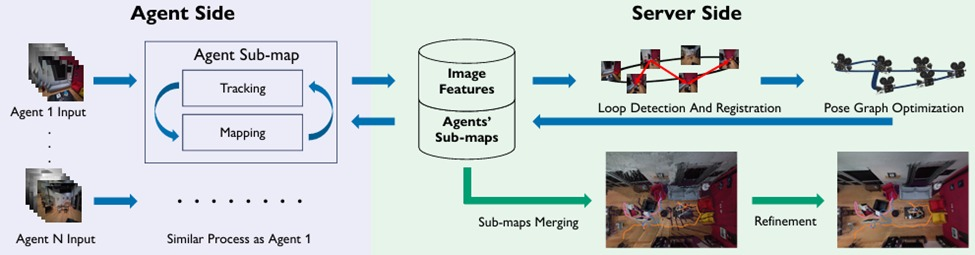
\includegraphics[width=0.8\textwidth]{magic.jpeg}
\caption{Overview of a multi-agent SLAM system~\cite{yugay2024magic}}
\label{fig:magic_slam}
\end{figure}

\subsection{Related Technology 11 -- WildGS-SLAM for Dynamic Environment Mapping}

WildGS-SLAM~\cite{zheng2025wildgs} addresses the challenge of SLAM in dynamic environments using a monocular camera and Gaussian splatting representation. Indoor delivery environments often include moving humans, doors which open and close and moving objects that are capable of corrupting the SLAM map. WildGS-SLAM proposes an uncertain tracking and mapping filter which identifies and eliminates dynamical features in the scene without the use of semantic segmentation or depth sensors. Through uncertainty prediction per-pixel, integrating it with dense bundle adjustment and Gaussian maps optimization, WildGS-SLAM performs a good tracking and high-fidelity mapping in dense indoor environments. This feature is very applicable in the parcel delivery robots which act in real-life enhighly moving and occluding environments.

\begin{figure}[H]
\centering
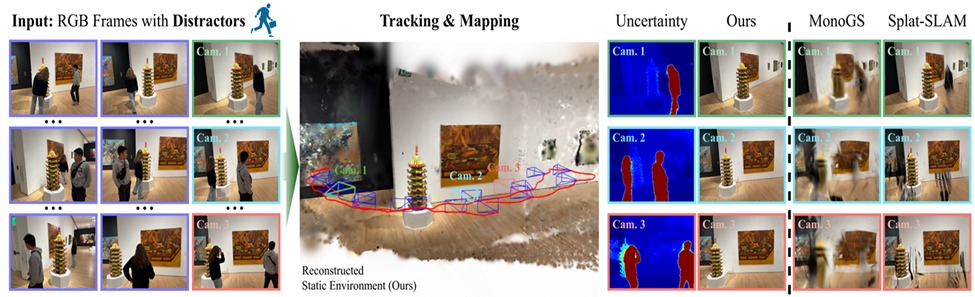
\includegraphics[width=0.8\textwidth]{wild gs.jpeg}
\caption{WildGS-SLAM Overview~\cite{zheng2025wildgs}}
\label{fig:wildgs_slam}
\end{figure}

\begin{table}[htbp]
\centering
\caption{Comparison of SLAM Techniques}
\label{tab:slam_comparison}
\begin{tabular}{|p{3cm}|p{3cm}|p{3cm}|p{3cm}|}
\hline
\textbf{SLAM Method} & \textbf{Strengths} & \textbf{Weaknesses} & \textbf{Application Suitability} \\
\hline
LiDAR-Based SLAM & High mapping accuracy & Expensive hardware & Industrial robotics \\
\hline
Visual SLAM & Cost-effective and flexible & Sensitive to lighting & Indoor mobile robots \\
\hline
DROID-SLAM & High accuracy and robustness & High computational req. & Auto navigation research \\
\hline
MAGiC-SLAM & Supports collaborative mapping & Complex implementation & Multi-robot systems \\
\hline
WildGS-SLAM & Handles moving objects & High processing cost & Dynamic indoor environments \\
\hline
\end{tabular}
\end{table}

Table~\ref{tab:slam_comparison} summarizes different SLAM techniques used for robot localization and mapping. LiDAR-based SLAM provides high accuracy but increases hardware cost. Visual SLAM offers cost-effective mapping using camera data but may be affected by lighting conditions. DROID-SLAM have enhanced accuracy and robustness mapping. Other multi-agent systems such as MAGiC-SLAM are improved collaborative mapping and WildGS-SLAM enhance the performance with respect to dynamic environments. These studies suggest that visual SLAM techniques are based on deep learning enable appropriate performance-cost tradeoff in indoor robotics.

\section{Related Projects}

There are a number of research projects and experimental robotic systems that have made a contribution significantly to the creation of autonomous perception systems, frameworks of navigation and mixed control policies. Such research provides valuable insights for middlewares integration, vision based perception, SLAM advancements, path planning strategies, among others, that impact the design of the proposed autonomous indoor parcel delivery system.

\begin{table}[htbp]
\centering
\caption{Comparative Summary of Related Research Projects in Autonomous Mobile Robot Navigation}
\label{tab:related_projects}
\begin{tabular}{|p{3cm}|p{4.5cm}|p{6cm}|}
\hline
\textbf{Project / Study} & \textbf{Techniques Used} & \textbf{Key Outcomes} \\
\hline
Bonci et al.~\cite{bonci2023ros2} & ROS2 middleware, modular architecture & Demonstrated ROS2 as a scalable platform enabling flexible integration \\
\hline
Gargouri et al.~\cite{gargouri2024cost} & ROS2 Nav2, AMCL, YOLO, fuzzy PID & Developed cost-effective indoor robot with reliable localization \\
\hline
Teed \& Deng~\cite{teed2021droid} & Deep learning visual SLAM, DBA & Provided highly accurate localization and mapping in complex environments \\
\hline
Yugay et al.~\cite{yugay2024magic} & Multi-agent SLAM, distributed mapping & Improved global map consistency and localization accuracy \\
\hline
Zheng et al.~\cite{zheng2025wildgs} & Gaussian splatting SLAM, dynamic filtering & Enhanced SLAM performance in dynamic environments \\
\hline
Cao et al.~\cite{cao2024pure} & Pure pursuit steering, reinforcement learning & Improved trajectory tracking and adaptive velocity control \\
\hline
Song et al.~\cite{song2020smooth} & Bezier curves, PSO optimization & Achieved smoother and kinematically feasible path generation \\
\hline
\end{tabular}
\end{table}

Table~\ref{tab:related_projects} summarizes major research contributions in autonomous mobile robot navigation, highlighting advancements in middleware frameworks, SLAM techniques, perception systems, and path planning methods. The studies reviewed prove the presence of the significance of ROS2 based modular designs, localization and mapping solutions and smarts in navigation. These developments, when added together, provide robust technological basis to develop trustworthy and effective autonomous directly underpin the process taken by the proposed project and are robotic systems.

\section{Related Studies / Research}

We investigated several research studies focusing on different aspects of navigation of autonomous mobile robots which will be useful to design and develop the indoor parcel delivery robot system.

\begin{itemize}
\item \textbf{Hybrid Path Planning Strategies:} In a comparative study, it has been demonstrated that a mixture of classical graph-based algorithms (such as A*) and optimization and learning-based approaches is appropriate.~\cite{ajeil2020grid}.Studies indicate that the hybrid navigation results in improved path optimality, adaptability and computational efficiency.
\item \textbf{Path Smoothing and Trajectory Optimization:}  We found that the raw paths usually contain discontinuities and sharp turns based on the work done on smoothing techniques for the smooth trajectories~\cite{ravankar2018path}. The researches show that the spline based interpolation and curve fitting methods improve the smoothness of the motion, decrease the mechanical stresses and enhance the tracking accuracy.
\item \textbf{PSO-Based Path Optimization:} A large number of studies have been conducted on the field of robot trajectory optimization using Particle Swarm Optimization (PSO)~\cite{song2020smooth}. It has been revealed that PSO can reduce both path length and curvature variation and also reduce energy consumption. The improved PSO variants exhibit faster convergence with better optimization ability.

\item \textbf{Dynamic Obstacle Avoidance in Indoor Environments:} The focus in human-aware navigation research is to incorporate vision sensors into the real-time obstacle avoidance algorithm.The problem of human-aware navigation focuses on the integration of vision-based perception systems with real-time obstacle avoidance algorithms~\cite{kumar2024real}. Research has shown that fusing computer vision models with adaptive motion planning enhances safety and reliability.

\item \textbf{ROS2-Based Autonomous Navigation Frameworks:} There have been a number of studies that have assessed ROS2 middleware for autonomous robotic applications~\cite{hwang2023ros2}. The studies show that ROS2 offers modular architecture, support for real-time communication and enhanced scalability.

\item \textbf{SLAM Performance in Indoor Navigation:} Comparative studies of visual SLAM, LiDAR-based SLAM, and deep learning-based SLAM methods indicate that visual SLAM provides a cost-effective solution for indoor localization~\cite{rosinol2020kimera}.

\item \textbf{Model Predictive Control for Mobile Robots:} MPC has been shown to be effective for handling motion constraints, optimizing the trajectory tracking and enhancing stability in the context of research~\cite{nascimento2023nonlinear}. The controller based on MPC is better than the classical PID controller.

\item \textbf{Simulation-Based Navigation Testing:} The relevance of simulation environments for testing robot navigation algorithms prior to deployment in the real world have been emphasized in the studies~\cite{park2021simulation}. The simulation platforms~\cite{koenig2004gazebo} enable the safe testing of SLAM, obstacle avoidance, and path planning strategies.
\end{itemize}

\section{Limitations and Bottlenecks of the Existing Work}
Although there are some great advancements in the field of autonomous mobile robot locomotion, some of the existing methods are constrained technically and practically and, thus, can only be effective in a real-world delivery scenario. These limitations can be related to difficulties in the optimisation of parameters, the quality of the path-generation, motion control stability, and environmental sensing. The detailed knowledge of these bottlenecks is invaluable to stipulate the areas in which a better navigation strategy and system architecture are justified.
\begin{table}[htbp]
\centering
\caption{Limitations of Existing Work}
\label{tab:limitations}
\begin{tabular}{|p{5cm}|p{9cm}|}
\hline
\textbf{Method / Approach} & \textbf{Limitation} \\
\hline
Default ROS2 Nav2 Framework & Requires extensive parameter tuning and offers limited flexibility for custom strategies \\
\hline
Traditional Path Planning (A*, Dijkstra, RRT) & Often generate jagged paths and show reduced efficiency in dynamic environments \\
\hline
Path Execution Without Smoothing & Produces trajectories that violate kinematic constraints, leading to unstable motion \\
\hline
Fixed-Gain Controllers & Lack adaptability to changing conditions, causing oscillations and poor tracking \\
\hline
Single-Sensor SLAM Methods & May suffer from localization drift or reduced performance in dynamic env. \\
\hline
Limited Dynamic Obstacle Handling & Classical systems often assume static env. and struggle with humans \\
\hline
Lack of Integrated Hybrid Nav Systems & Most studies focus on individual components rather than unified frameworks \\
\hline
\end{tabular}
\end{table}

See Table~\ref{tab:limitations} for the limitations, suggesting a need for more adaptive, integrated, and optimization-driven navigation solutions. To tackle these challenges, advanced perception techniques, smooth and fast route planning, adaptive obstacle management and enhanced adaptive control and dynamic control systems are needed. These observations are one of the most motivating factors that will trigger the development of the proposed autonomous delivery robot system, which aims to overcome these limitations by adopting a hybrid navigation approach and enhancing system integration.

\section{Problem Statement}

Even though the current robotic middleware applications like ROS 2 and the Navigation 2 (Nav2) architecture offer good baseline navigation functions, a number of technical challenges remain. Delivery of parcels manually in large indoor areas is time-consuming, labor intensive and prone to delays. The majority of the current implementations are dependent on pre-configured navigation modules which restricts flexibility of the system. Existing autonomous delivery solutions have severe constraints, including path jagging which breaks the kinematic limit of differentially-driven robots. The additional effects of path smoothing and trajectory optimization are unstable in robot motion. Moreover, a lot of implementations cannot deal with dynamic obstacle avoidance. Localization accuracy is also a major problem, especially when it comes to visual static or dynamic environments. More so, traditional methods of motion control like fixed-gain controllers demand a lot of parameter adjustment. To address these challenges, this project will provide an integrated solution with ROS 2 middleware-based robot that encompasses effective SLAM-based localization and hybrid path planning.

\section{Summary}

In this chapter, literature review was discussed including the principles of autonomous mobile robots navigation such as robotic perception, localization (SLAM) and path planning, trajectory smoothing and motion control strategies have been discussed. It also examined ROS 2 middlewares and simulation tools helpful in autonomous robot operation. The comparison of similar projects and research works provided information about the necessity of combining localization, planning, control, and perception modules. The shortcomings of the current navigation methods underscore the necessity to establish incorporated and more tailored navigation systems. Hence, the proposed project will be aimed at the deploying of a ROS 2-based autonomous parcel delivery robot as a solution to the existing gap between the theoretical concepts of navigation and the real-world application of robots.
	\chapter{PROJECT DESIGN AND IMPLEMENTATION}
\label{ch:Project Design and Implementation}
This chapter presents the design and implementation of the autonomous parcel delivery navigation system. It covers the development approach, performance metrics, software architecture, algorithm design, simulation setup, and prototype demonstration. The chapter explains the step-by-step development process and testing methods used to ensure the system operates reliably and efficiently in complex indoor environments.
\section{Proposed Design Methodology}

The parcel delivery system design method combines a web management integration system, the ROS2 (Robot Operating System 2) navigation system, along with a web-based simulation and visualization of autonomous navigation and a web-based automation system. The system integrates management, real-time monitoring of delivery robots, map management, and the ability to visualize robot operations.

Figure~\ref{overall}At the top are the live telemetry and task options along with the maps and logs which are all accessible via the web interface. The web interface is connected to the backend in Flask. From there it's application logic, REST APIs and database, as well as interface between the web and ROS2. The communication layer robs towards the coordination for the navigation stack, the Gazebo simulation, RViz, and the TurtleBot3. The components of the navigation stack are the Improved A* with Particle Swarm Optimization (PSO) for path smoothing, and Model Predictive Controller (MPC) for path and tracking. The simulation for the navigation of the robot is provided by Gazebo, while the visualizations by RViz for the maps, planned paths, and the robot's telemetry are also real time.
The project is outlined into six development stages:

\begin{figure}[H]
	\centering
	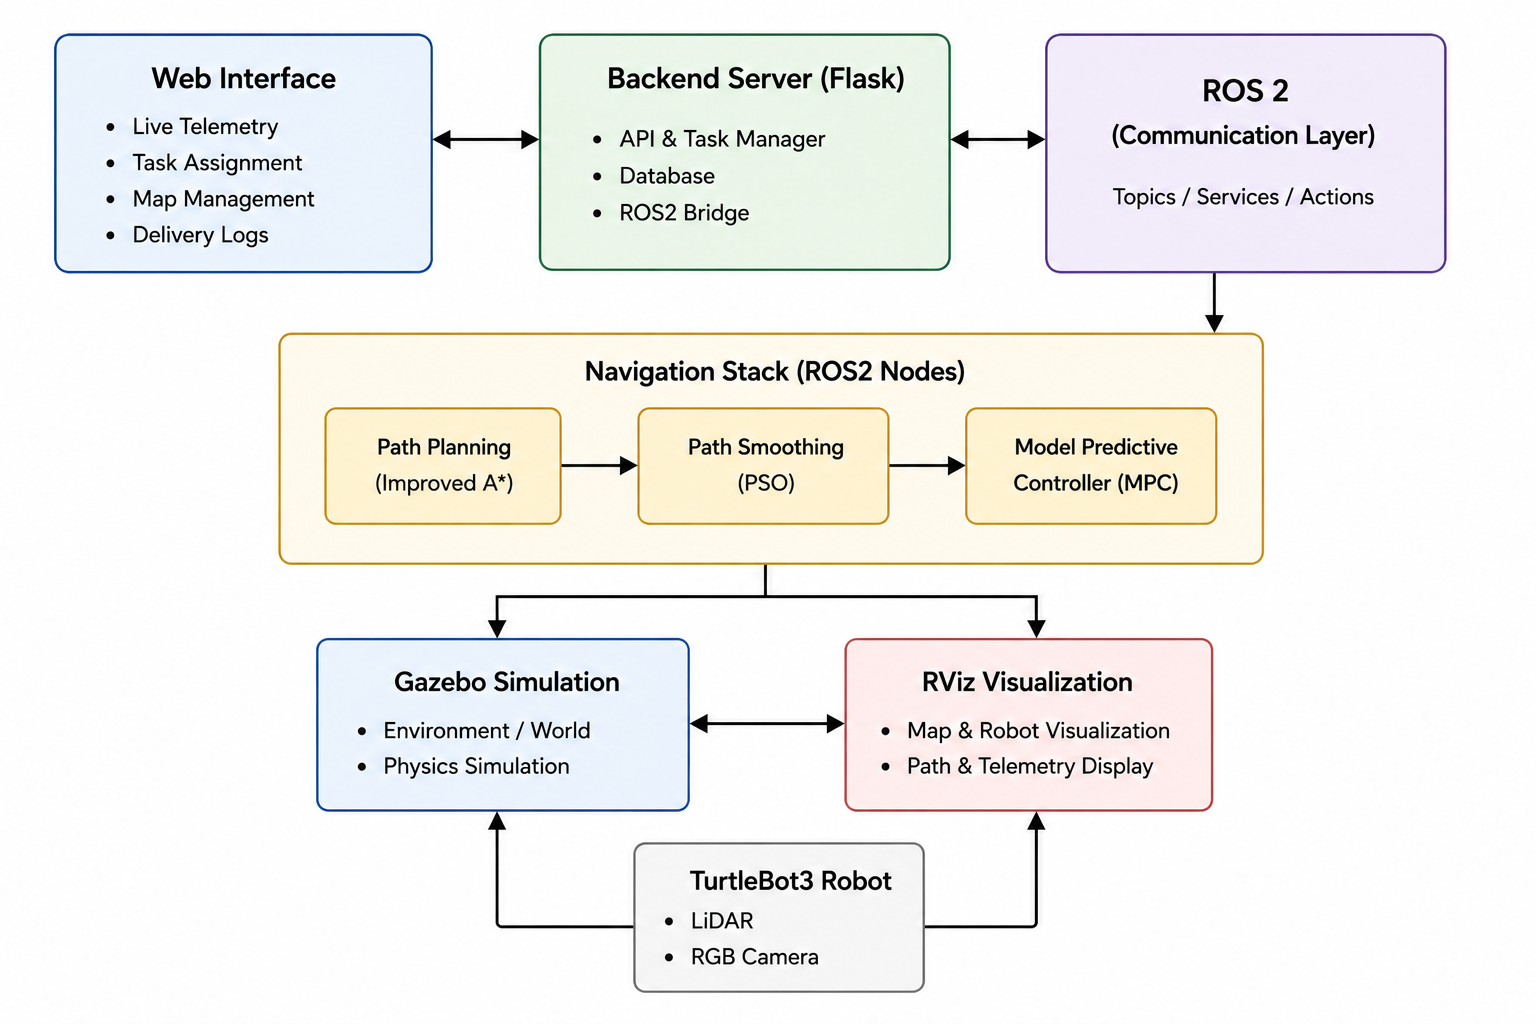
\includegraphics[width=1\textwidth]{overall architecture.png}
	\caption{Overall Architecture of the Proposed Autonomous Parcel Delivery System}
	\label{overall}
\end{figure}

\subsection*{Phase 1: Navigation Algorithm Development}

To create collision-free global paths in the simulation, the Improved A* path planning algorithm was applied. Then, Particle Swarm Optimization (PSO) path smoothing was used to create paths that were shorter, smoother, and more practical for autonomous navigation.
\subsection*{Phase 2: Web-Based Management Platform Development}

A Flask-based application based on Flask for users to easily assign delivery tasks, view real time delivery robot telemetry, manage occupancy maps, and view delivery logs. The interface is the main point of user interaction with the autonomous delivery system.

\subsection*{Phase 3: Backend and ROS2 Integration}

To create smooth connection between the online platform and the robotic system, the backend server was linked with ROS2. While robot status and telemetry data are continuously sent back to the web interface, user commands, delivery objectives, and map management requests are routed to ROS2.

\subsection*{Phase 4: Model Predictive Control Implementation}

To precisely track the optimum navigation path produced by the planning module, a Model Predictive Controller (MPC) was put into place. Smooth and stable autonomous mobility is achieved by the controller's computation of suitable velocity commands while meeting the robot's kinematic limitations.

\subsection*{Phase 5: Simulation and Visualization Integration}
Gazebo and RViz were integrated with the entire navigation stack. While RViz delivers real-time viewing of occupancy maps, robot position, planned trajectories, and navigation status during autonomous deliveries, Gazebo offers a realistic simulation environment for assessing robot performance.


\subsection*{Phase 6: System Deployment and Validation}

Ubuntu 22.04, ROS2, Gazebo, and the TurtleBot3 robot model with LiDAR and RGB camera sensors were used to implement the whole autonomous package delivery system. To verify task execution, autonomous navigation, path tracking, and communication between the web interface and the robotic platform, end-to-end testing was carried out.



\subsection{Overall System Architecture}

A web-based user interface, backend processing, robotic middleware, simulation environment, and the autonomous mobile robot are all integrated into the modular architecture of the suggested autonomous parcel delivery system. Figure~\ref{fig:system_architecture} shows the general workflow of the suggested system, starting with the assignment of tasks to users and concluding with the effective completion of deliveries.

In order to assign delivery jobs and track the robot's real-time telemetry during the delivery process, the user engages with the Web Interface at the highest level. The Backend, which handles user requests and acts as a communication link between the web application and the robotic system, is communicated with using the web interface.

The ROS2 Communication Layer, which serves as the middleware in charge of information exchange between the robot and the software components, is integrated with the backend. In the Gazebo Simulation environment, where the TurtleBot3 robot completes autonomous parcel delivery tasks under realistic simulation conditions, the navigation system is assessed.

The TurtleBot3 Robot has an RGB camera for visual perception and a LiDAR sensor for obstacle recognition and localization. The robot automatically follows the designated delivery path and arrives at the designated destination using the navigation algorithms built into the ROS2 framework, all the while continuously sending telemetry updates to the web interface.

User interaction, backend services, robotic middleware, simulation, and robot operation are all clearly separated thanks to this modular architecture. Scalability, maintainability, and future integration with actual robot hardware are all enhanced by such a design.


\begin{figure}[H]
	\centering
	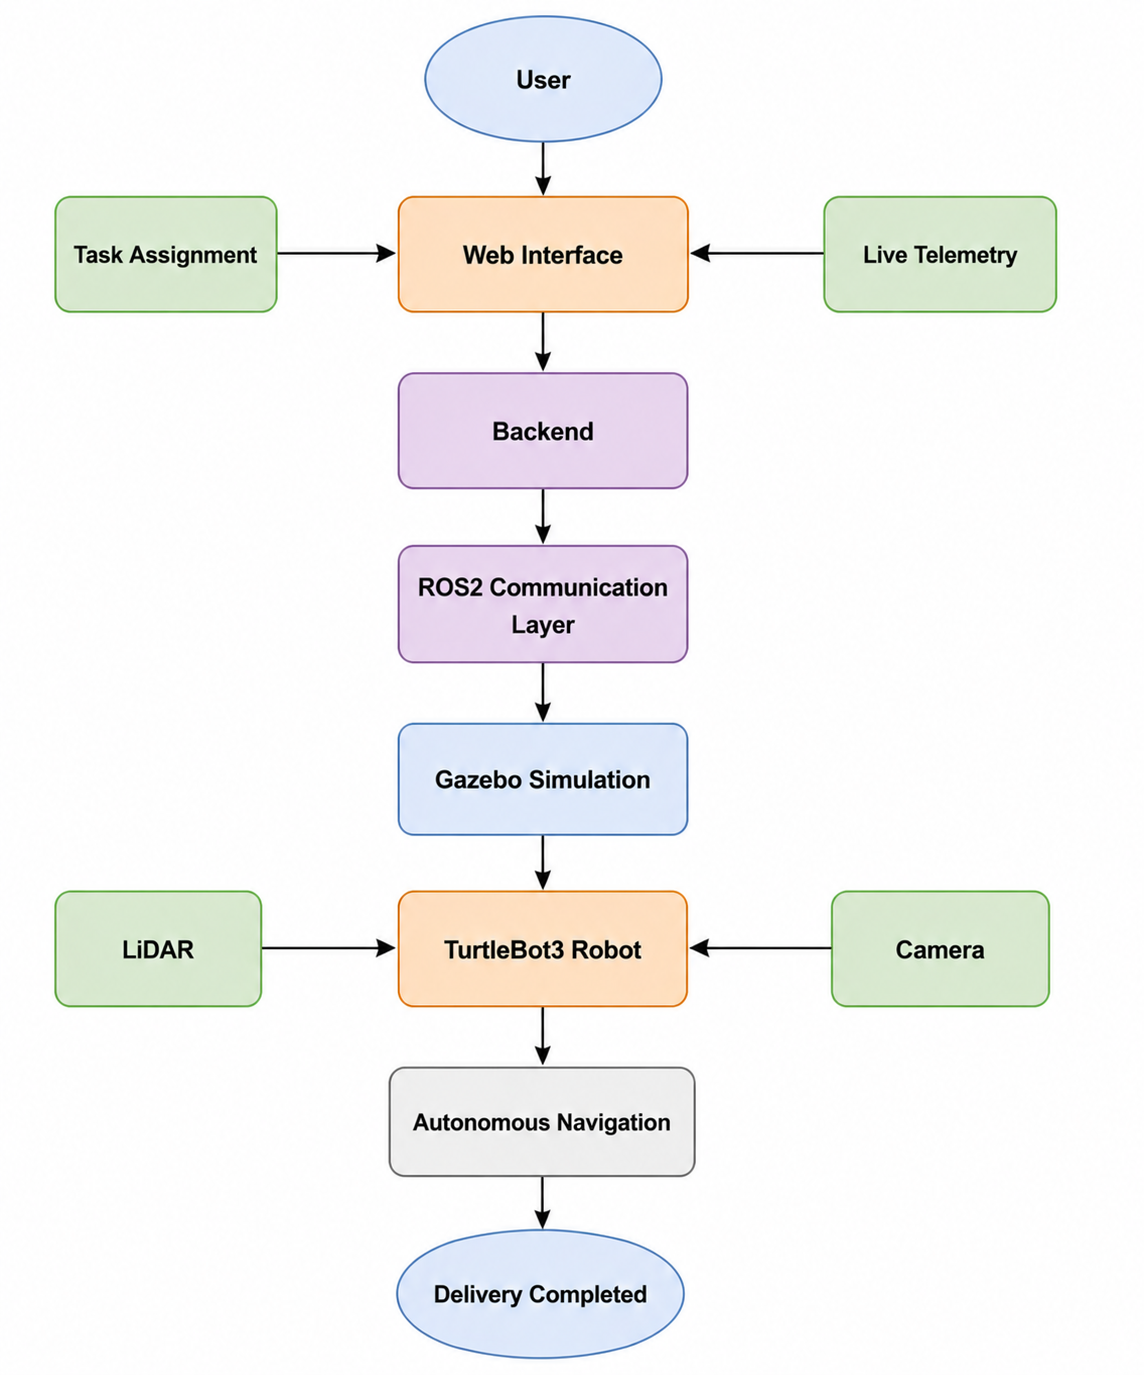
\includegraphics[width=0.8\textwidth]{overflow.png}
	\caption{Overall System Architecture of the Proposed Autonomous Parcel Delivery System}
	\label{fig:system_architecture}
\end{figure}
\section{Implementation Procedure}
\section{Phase 1: Global Path Planning}
\label{sec:phase1_astar}

The global route planning module, which is the first part of the six-phase development approach, is fully designed and implemented in this section. The global planner in charge of creating collision-free pathways throughout the occupancy grid representation of the workspace was chosen to be the Improved A* (IA*) algorithm.


\subsection{Why A*}
\label{subsec:why_astar}

For global path planning, A* algorithm was implemented for its heuristic search efficiency and optimality guarantees. In contrast to ignorant search algorithms like Dijkstra's algorithm, A* employs a heuristic function to steer the search in the direction of the objective. When an admissible heuristic is employed, this drastically reduces the number of nodes examined while still ensuring the shortest path.

The following are the main justifications for using A* as the global planner:


\begin{itemize}[noitemsep]
\item \textbf{Optimality:} When employing an acceptable heuristic (Euclidean distance), A* ensures the shortest collision-free path between the start and target nodes.
\item \textbf{Completeness:} If there is a solution in the occupancy grid, the algorithm will discover it.
\item \textbf{Heuristic-guided efficiency:} Compared to exhaustive search techniques, the Euclidean distance heuristic reduces computer overhead by focusing the search on the objective.
\item \textbf{Grid compatibility:} A* is readily suitable to the workspace representation used in this project because it functions natively on discretized occupancy grid maps.
\item \textbf{Deterministic behavior:} A* simplifies testing and validation by generating repeated, consistent paths for a given map and start/goal setup.

\end{itemize}

In order to overcome the discontinuities and abrupt turns that come with grid-based planning, A* was used as the main global path planner. Its output was then improved through path trimming and PSO-based smoothing (Phase 2).



\subsection{A* Implementation}
\label{subsec:astar_implementation}

A grid-based workspace representation is used in the Python implementation of the A* path planning algorithm. A consistent grid with adjustable resolution is created by discretizing the environment. Based on the locations of obstacles, each grid cell is categorized as either occupied or free area. The technique employs a priority queue to choose nodes with the lowest cost function while maintaining open and closed sets for node exploration:


\begin{equation}
	f(n) = g(n) + h(n)
	\label{eq:astar_cost_impl}
\end{equation}

where $g(n)$ is the actual cost from the start node to the current node, and $h(n)$ is the heuristic estimate from the current node to the goal node.

\subsubsection*{Path Pruning}

Path pruning is employed to remove redundant waypoints produced by A* algorithm. This is done by the pruning algorithm. It goes from one waypoint to the next deleting intermediate spots that do not improve the path quality. A line-of-sight check is performed to ensure a collision-free connection between non-consecutive waypoints.


\subsubsection*{Backend Implementation File}

The backend implementation of the A* algorithm is in \texttt{astar\_modified.py}, which contains the modified A* path planning algorithm tailored to the specific constraints of the project (dynamic safety margin, adaptive grid resolution and 8-directional motion model, see Section ~\ref{subsec:astar_parameters}).


\subsection{Mathematical Model}
\label{subsec:astar_math_model}

The path planning process is modeled as a graph search problem where the environment is divided into a discrete grid. The A* algorithm evaluates nodes using the cost function:

\begin{equation}
	f(n) = g(n) + h(n)
	\label{eq:astar_cost}
\end{equation}

where:
\begin{itemize}[noitemsep]
	\item $g(n)$ = actual cost from start node to current node
	\item $h(n)$ = heuristic estimate from current node to goal node
\end{itemize}

The Euclidean distance heuristic is used, as it is admissible (never overestimates the true cost) and thus preserves the optimality of the A* search:

\begin{equation}
	h(n) = \sqrt{(x_{goal} - x_{current})^2 + (y_{goal} - y_{current})^2}
	\label{eq:euclidean_heuristic_p1}
\end{equation}

Dynamic programming techniques are used to store optimal sub-path solutions, improving computational efficiency through memoization.

\subsection{Parameters}
\label{subsec:astar_parameters}

The A* path planning algorithm is configured with the following adaptive parameters:

\begin{description}[leftmargin=0cm, labelindent=0cm, itemsep=0.3em, font=\normalfont]
	\item[Grid Resolution:] The grid resolution adapts to workspace dimensions to balance computational efficiency and path accuracy:
	\begin{equation}
		\text{resolution} = \min(\text{width}, \text{height}) \times 0.01
	\end{equation}
	
	\item[Safety Margin:] A dynamic safety margin is applied around obstacles to prevent collisions:
	\begin{equation}
		\text{safety\_margin} = \text{resolution} \times 0.2 \text{ meters}
	\end{equation}
	
	\item[Motion Model:] The robot uses an 8-directional motion model with diagonal movement cost of $\sqrt{2} \times \text{resolution}$.
	
	\item[Grid Indexing Formula:] Each cell is assigned a unique index for efficient lookup:
	\begin{equation}
		\text{index} = y_{\text{index}} \times x_{\text{width}} + x_{\text{index}}
	\end{equation}
	
	\item[Heuristic Function:] Euclidean distance is used as the admissible heuristic for optimal pathfinding.
\end{description}

Table~\ref{tab:astar_parameters} summarizes the A* configuration parameters.

\begin{table}[H]
	\centering
	\caption{A* Algorithm Parameters and Configuration}
	\label{tab:astar_parameters}
	\begin{tabular}{|p{4cm}|p{3cm}|p{6.5cm}|}
		\hline
		\textbf{Parameter} & \textbf{Type} & \textbf{Value/Formula} \\
		\hline
		Grid Resolution & Adaptive & $\min(\text{width}, \text{height}) \times 0.01$ \\
		\hline
		Safety Margin & Dynamic & $\text{resolution} \times 0.2$ m \\
		\hline
		Motion Model & 8-directional & Diagonal cost $= \sqrt{2} \times \text{resolution}$ \\
		\hline
		Heuristic Function & Euclidean & $\sqrt{(x_g - x_c)^2 + (y_g - y_c)^2}$ \\
		\hline
		Grid Indexing & Formula & $y_{index} \times x_{width} + x_{index}$ \\
		\hline
	\end{tabular}
\end{table}


\section{Phase 2: Path Optimization}
\label{sec:phase2_optimization}

Following global path generation by the A* planner (Section~\ref{sec:phase1_astar}), the raw path is refined through a two-stage optimization pipeline: path pruning to eliminate redundant waypoints, followed by Particle Swarm Optimization (PSO)-based smoothing to produce a continuous, kinematically feasible trajectory suitable for differential-drive robot motion.

\subsection{Path Pruning}
\label{subsec:path_pruning}

On an 8-directional grid, the raw path produced by A* usually has a lot of closely spaced, collinear, or near-collinear waypoints that are not necessary for smooth trajectory execution and are computationally costly to monitor. Prior to PSO smoothing, path pruning is used as the initial optimization step to minimize this redundancy.

The pruning method eliminates intermediate points that don't improve path quality by iterating through successive waypoints. To ensure collision-free connection, a line-of-sight check is carried out between non-consecutive waypoints. All intermediate waypoints between two non-adjacent waypoints are eliminated if a straight line between them does not cross any obstacles (within the safety margin).
By eliminating needless zigzag segments added by the grid-based search, this step considerably lowers waypoint density while also somewhat reducing the overall path length.


\subsection{Results}
\label{subsec:astar_results}

The A* global planner was tested in two simulated indoor test scenarios of different complexity and scale with the path planning performance indicators (path length, waypoint density, and computing efficiency). The pruned path (after removing redundant waypoints, see Section~\ref{subsec:astar_implementation}) and the raw output of the A* were both recorded for comparison.

\subsubsection*{Scenario 1: M4 Map (100 $\times$ 100 m)}

\textbf{Start:} $(35.0, 95.0)$ \quad \textbf{Goal:} $(50.0, 8.0)$ \\
\textbf{Grid Resolution:} 2.0 m \quad \textbf{Safety Margin (Inflation):} 3.0 m

\begin{table}[H]
	\centering
	\caption{A* Path Planning Results -- Scenario 1 (M4 Map)}
	\label{tab:astar_results_scenario1}
	\begin{tabular}{|p{4.5cm}|p{4cm}|p{4cm}|}
		\hline
		\textbf{Metric} & \textbf{Raw A* Path} & \textbf{Pruned A* Path} \\
		\hline
		Path Length & 100.62 meters & 96.13 meters \\
		\hline
		Waypoint Count & 47 waypoints & 6 waypoints \\
		\hline
		\multicolumn{3}{|c|}{Computation Time: IA* $\approx$ 0.1346 s \quad A* $\approx$ 0.1410 s} \\
		\hline
	\end{tabular}
\end{table}

\subsubsection*{Scenario 2: Mobile Robot Workspace (160 $\times$ 160 m)}

\textbf{Start:} $(5.0, 155.0)$ \quad \textbf{Goal:} $(155.0, 5.0)$ \\
\textbf{Grid Resolution:} 3.0 m \quad \textbf{Safety Margin (Inflation):} 3.0 m

\begin{table}[H]
	\centering
	\caption{A* Path Planning Results -- Scenario 2 (Mobile Robot Workspace)}
	\label{tab:astar_results_scenario2}
	\begin{tabular}{|p{4.5cm}|p{4cm}|p{4cm}|}
		\hline
		\textbf{Metric} & \textbf{Raw A* Path} & \textbf{Pruned A* Path} \\
		\hline
		Path Length & 244.99 meters & 233.87 meters \\
		\hline
		Waypoint Count & 69 waypoints & 5 waypoints \\
		\hline
		\multicolumn{3}{|c|}{Computation Time: IA* $\approx$ 0.4181 s \quad A* $\approx$ 0.4135 s} \\
		\hline
	\end{tabular}
\end{table}

\subsubsection*{Key Observations}

\begin{itemize}[noitemsep]
\item \textbf{Identical paths between planners:} In all cases, the Improved A* (IA*) planner and the conventional A* planner produce similar paths (with the same length and number of waypoints) because obstacles prevent a straight line from start to goal, and both planners are forced to rely on the entire grid search. The difference in computation time between the two planners is minimal.
\item \textbf{Effectiveness of pruning:} The path pruning step reduces significantly the waypoint density and the total path length by eliminating useless zigzag segments generated by the 8-directional grid search:

\begin{itemize}[noitemsep]
	\item In Scenario~1, waypoint pruning reduced the number of waypoints from 47 to 6, representing an 87.2\% reduction, while shortening the path length by 4.49~m, from 100.62~m to 96.13~m.
	
	\item In Scenario~2, waypoint pruning reduced the number of waypoints from 69 to 5, corresponding to a 92.8\% reduction, and decreased the path length by 11.12~m, from 244.99~m to 233.87~m.
\end{itemize}	
\end{itemize}

\subsection{Particle Swarm Optimization (PSO)}
\label{subsec:pso_overview}
Pruning will eliminate useless waypoints, but the resulting path may contain sharp turns and discontinuities of the curvature that are incompatible with the kinematic specifications of a differential-drive robot. The path is further smoothed by the aid of Particle Swarm Optimization (PSO) for improving the trajectory feasibility and reducing the sharp curves.

Each swarm particle is a candidate smoothed path and the position variables of each particle are the coordinates of the way points between the smoothed path particles. Each iteration, the swarm updates the position of each particle according to the velocity equations, all the while keeping an eye on a cost function that combines path length, smoothness and obstacle proximity. The swarm moves towards a path which is balancing these conflicting goals.
\subsection{Cost Function}
\label{subsec:pso_cost_function}

The PSO smoothing process optimizes a multi-objective cost function that is a combination of three weighted components:

\begin{equation}
	J = w_1 \cdot L + w_2 \cdot C + w_3 \cdot P
	\label{eq:pso_cost_p2}
\end{equation}

where:
\begin{itemize}[noitemsep]
	\item $L$ = total path length
	\item $C$ = curvature or smoothness factor
	\item $P$ = obstacle penalty function
	\item $w_1, w_2, w_3$ = weighting coefficients
\end{itemize}

Smaller values of $J$ correspond to shorter, smoother and safer routes. The penalty term $P$ for obstacle grows rapidly when the candidate path is close to or crosses an obstacle boundary, discouraging the swarm from converging to infeasible trajectories.

\subsection{Equations}
\label{subsec:pso_equations}

Particle position and velocity updates follow the standard PSO formulation:

\begin{align}
	v_i(t+1) &= w \cdot v_i(t) + c_1 \cdot r_1 \cdot (p_{best,i} - x_i(t)) + c_2 \cdot r_2 \cdot (g_{best} - x_i(t)) \label{eq:pso_velocity_p2} \\
	x_i(t+1) &= x_i(t) + v_i(t+1) \label{eq:pso_position_p2}
\end{align}

where:
\begin{itemize}[noitemsep]
	\item $w$ = inertia weight, controlling the influence of a particle's previous velocity
	\item $c_1, c_2$ = cognitive and social coefficients, weighting a particle's attraction to its own best-known position and the swarm's best-known position respectively
	\item $r_1, r_2$ = random values in $[0,1]$, introducing stochastic variation into the search
	\item $p_{best,i}$ = personal best position found by particle $i$
	\item $g_{best}$ = global best position found by the entire swarm
\end{itemize}

At each iteration, every particle's cost $J$ (Equation~\ref{eq:pso_cost_p2}) is evaluated, and $p_{best,i}$ and $g_{best}$ are updated whenever a particle discovers a lower-cost path. This process repeats until a maximum number of iterations is reached or convergence criteria are satisfied.

\subsection{Parameters}
\label{subsec:pso_parameters}

Particle Swarm Optimization is configured with the following parameters to balance exploration and exploitation:

\begin{table}[H]
	\centering
	\caption{PSO Algorithm Parameters}
	\label{tab:pso_parameters_p2}
	\begin{tabular}{|p{6cm}|p{2cm}|p{2cm}|}
		\hline
		\textbf{Parameter} & \textbf{Symbol} & \textbf{Value} \\
		\hline
		Swarm Size & $N_p$ & 50 particles \\
		\hline
		Maximum Iterations & $I_{max}$ & 100 \\
		\hline
		Inertia Weight & $w$ & 0.7 \\
		\hline
		Cognitive Coefficient & $c_1$ & 1.5 \\
		\hline
		Social Coefficient & $c_2$ & 1.5 \\
		\hline
		Weight -- Path Length & $w_1$ & 0.5 \\
		\hline
		Weight -- Smoothness & $w_2$ & 0.3 \\
		\hline
		Weight -- Obstacle Penalty & $w_3$ & 0.2 \\
		\hline
	\end{tabular}
\end{table}

\subsection{Implementation}
\label{subsec:pso_implementation}

Particle Swarm Optimization's Python implementation smooths the navigation trajectories. Each particle represents a potential smoothed path, and the particle's search space is made up of the positional variables that make up the path's intermediate nodes. The swarm uses the velocity update equations to compute particle positions across a number of iterations.
 (Equations~\ref{eq:pso_velocity_p2}--\ref{eq:pso_position_p2}), while simultaneously evaluating the cost function (Equation~\ref{eq:pso_cost_p2}) combining path length, curvature, and obstacle proximity.

The PSO smoothing module is implemented in the backend and provides an optimized, smoothed trajectory to be sent to the MPC trajectory tracking controller (Phase 4) after receiving the pruned waypoint list from the path pruning stage.

\subsection{Path Planning Performance Metrics}

The effectiveness of path planning is assessed by looking at the generated paths' quality and viability. Verification of collision-free navigation, path length reduction, and computational efficiency are the goals of this test.
The following measures are used to assess path planning performance:


\subsubsection{Path Length}


Path length is a distance that a robot traverses on the plan. It is computed by adding the breakeven distance among successive waypoints. The shortest routes are desirable because they save on time of travel and energies.
\subsubsection{Collision-Free Validation}

The consequent pathway is confirmed with the boundaries of obstacles by carrying out geometric intersection detection algorithms. The path must ensure that there is a small safety margin compared to all the hazards in an attempt to prevent the occurrence of collisions when running.

\subsubsection{Waypoint Density}

The density of the waypoints measures the number of intermediate nodes that are put in place along the route. Excessive number of waypoints means the system is prone to high computing loads in tracking the trajectories and insufficient number of waypoints may undermine the accuracy of the route especially in complex environments.
\subsection{Path Optimization and Smoothness Evaluation}

The path optimization analysis discussed below focuses on path optimization done after the global path generation. This will be done to achieve a better smoothness and minimise sudden direction changes hence, to better track trajectory performance and mechanical stress of the robot.  

The efficacy of the optimization is assessed using the following measures:  

\subsubsection{Curvature Continuity}

The change in curvature in successive path segments is studied to determine the directional consistency. Reduction in the curvature discontinuities is an indication of a smoother transition, which makes the trajectory applicable to the differential-drive robots.  

\subsubsection{Turning Angle Analysis}

Angles between path segments are calculated between successive path segments. Smaller turning angles represent smoother routes and it follows that such routes demand less aggressive steering inputs.  


\section{Phase 3: Controller Design}
\label{sec:phase3_mpc}

After the global path is planned (Phase 1) and smoothed (Phase 2), a Model Predictive Controller (MPC) is designed to make the robot follow this path accurately. The controller makes sure the robot moves smoothly, stays close to the planned path, and never asks the robot to move faster or turn sharper than it physically can. This section explains the robot model, the math behind the MPC, its limits, its settings, and how it was built.

\subsection{Robot Model}
\label{subsec:mpc_robot_model}

This project uses the \textbf{TurtleBot3 Waffle} robot. It is a differential-drive robot, meaning it moves using two wheels that can be driven at different speeds. Because of this design, the robot cannot move sideways -- it can only move forward/backward and turn, based on its linear speed and turning speed. This is called a non-holonomic robot. The MPC controller is designed around this simple but realistic motion behavior.

\subsection{Kinematics}
\label{subsec:mpc_kinematics}

The basic equations describing the robot’s motion are:

\begin{align}
	\dot{x} &= v \cos(\theta) \label{eq:mpc_kinematic_x} \\
	\dot{y} &= v \sin(\theta) \label{eq:mpc_kinematic_y} \\
	\dot{\theta} &= \omega \label{eq:mpc_kinematic_theta}
\end{align}

where:
\begin{itemize}[noitemsep]
	\item $x, y$ = the robot's position
	\item $\theta$ = the direction the robot is facing
	\item $v$ = forward speed
	\item $\omega$ = turning speed
\end{itemize}

Since the controller works in small time steps, these equations are converted into a step-by-step (discrete) form using simple time-stepping (Euler integration):

\begin{align}
	x_{k+1} &= x_k + v_k \cos(\theta_k) \, \Delta t \\
	y_{k+1} &= y_k + v_k \sin(\theta_k) \, \Delta t \\
	\theta_{k+1} &= \theta_k + \omega_k \, \Delta t
\end{align}

Here $\Delta t$ is the time between each step, and $k$ means "step number." This step-by-step version is what the MPC actually uses internally to guess the robot's future position.

\subsection{MPC Equations}
\label{subsec:mpc_equations}

MPC works by looking a few steps into the future, checking many possible ways the robot could move, and picking the one that follows the path best while also moving smoothly. Only the very first move of that plan is actually used -- then the controller repeats the whole process again at the next time step. This is known as receding horizon approach.

The controller tries to minimize this cost:

\begin{equation}
	\min_{u} \sum_{k=0}^{N-1} \left( \|x_k - x_{ref}\|^2_Q + \|u_k\|^2_R + \|\Delta u_k\|^2_S \right)
	\label{eq:mpc_cost_p3}
\end{equation}

In simple terms, this equation adds up three types of "penalties" over the next $N$ steps and tries to keep the total as low as possible:

\begin{itemize}[noitemsep]
	\item $x_k$ = the robot's predicted state (position, heading, speed) at step $k$
	\item $x_{ref}$ = the target point on the smoothed path (from Phase 2)
	\item $u_k$ = the control command at step $k$: acceleration $a$ and turning speed $\omega$
	\item $\Delta u_k = u_k - u_{k-1}$ = how much the command changes from one step to the next
	\item $Q$ = penalty for being far from the path
	\item $R$ = penalty for using large control effort
	\item $S$ = penalty for sudden, jerky changes in control
	\item $N$ = how many steps ahead the controller looks (prediction horizon)
\end{itemize}

So: $Q$ keeps the robot on track, $R$ keeps its movements gentle, and $S$ keeps its movements smooth and non-jerky.

\subsection{Constraints}
\label{subsec:mpc_constraints}
In solving the above optimization problem, the controller must meet the following constraints:

\begin{itemize}[noitemsep]
	\item The predicted robot motion should confirm to the kinematic model (Equations~\ref{eq:mpc_kinematic_x}--\ref{eq:mpc_kinematic_theta}).
	\item \textbf{Velocity limits:} $0 \leq v \leq 0.22$~m/s and $-2.84 \leq \omega \leq 2.84$~rad/s.
	\item \textbf{Obstacle avoidance:} The predicted path has to be kept at a safe distance from all known obstacles.
\end{itemize}
These limits make sure the commands the MPC generates are things the TurtleBot3 Waffle can actually do, and that the robot never plans a path through an obstacle.

\subsection{Parameters}
\label{subsec:mpc_parameters}

The impact of the MPC tuning profiles on the path-following performance of the robot was examined. Each profile changes the robot’s smoothness and how closely it follows the path it is supposed to follow.

\begin{table}[H]
	\centering
	\caption{MPC Tuning Profiles}
	\label{tab:mpc_profiles}
	\begin{tabular}{|p{3.8cm}|c|c|p{5.2cm}|}
		\hline
		\textbf{Profile} & \textbf{$Q_x,Q_y$} & \textbf{$R,\;S$} & \textbf{Purpose} \\
		\hline
		Calibrated Tuning & 500 & (0.1, 1.0) & Balanced performance for normal path following. \\
		\hline
		Glue-to-Path & 2500 & (0.01, 0.05) & Reduces corner cutting and improves path adherence. \\
		\hline
		Strict Glue-to-Path & 2500 & (0.01, 0.01) & Provides the tightest path-following behavior. \\
		\hline
	\end{tabular}
\end{table}
The Calibrated Tuning profile is good for general navigation and provides a good balance of performance. The robot stays closer to the intended path while turning fewer corners thanks to the Glue-to-Path profile, which boosts the position-tracking weight. Out of the three profiles, the Strict Glue-to-Path profile produces the most precise path-following behavior by strengthening route tracking and reducing control variances.



\subsection{Implementation}
\label{subsec:mpc_implementation}

Using common optimization libraries, the MPC controller is written in Python. The prediction step of the controller incorporates the robot's kinematic model (Section~\ref{subsec:mpc_kinematics}), and each time the controller operates, the speed/control-change restrictions from the selected tuning profile (Section~\ref{subsec:mpc_parameters}) are enforced.

The controller performs this action every control cycle: In short:



\begin{enumerate}[noitemsep]
	\item Reads the current position, heading and speed of the robot Reads the next section of the target path (from Phase 2)
	\item Predicts what will happen in the next $N$ steps with the kinematic model.
	\item  Solves the optimization problem (Equation~\ref{eq:mpc_cost_p3}) with the $Q$, $R$ and $S$ values of the selected profile to find the best sequence of moves.
	\item Uses only the very first move $u_0 = (a_0, \omega_0)$ from that sequence and sends it to the robot.
	\item Moves the prediction window one step forward and repeats the whole process again.
\end{enumerate}

The robot's mobility is precise and fluid because the controller continuously replans at each stage, allowing it to automatically adapt to minor mistakes or unforeseen disruptions. Depending on what is required, the system can trade off between very tight path following and softer, smoother control by switching between the three tuning profiles.




\section{Phase 4: Web Interface and Backend Implementation}

The web-based interface has been designed to provide users with a user-friendly platform to plan navigation environments, manage delivery rooms, dispatch delivery tasks, and monitor the robot in real time. The system follows a client-server architecture, with a clear separation between the Flutter frontend, the Flask backend, and the ROS2 robotic middleware. The complete frontend is delivered as a single Flutter web application named \textbf{ParcelPath} a real-time, autonomous indoor delivery management portal through which end users request and track deliveries and administrators configure and monitor the robot.

\subsubsection{Frontend and Backend Technology Stack}

Table~\ref{tab:web_stack} presents the technology stack used for developing the web platform.

\begin{table}[H]
	\centering
	\caption{Web Platform Technology Stack}
	\label{tab:web_stack}
	\begin{tabular}{|p{3cm}|p{4.5cm}|p{6.5cm}|}
		\hline
		\textbf{Component} & \textbf{Technology} & \textbf{Responsibility} \\
		\hline
		Frontend & Flutter (Dart), Provider state management & User interface, interactive map canvas, delivery requests, real-time robot tracking \\
		\hline
		Backend & Python (Flask), SQL & REST API handling, delivery FSM logic, path-planning execution, database management \\
		\hline
		Database & SQLite & Persistent storage for users, rooms, deliveries, orders, and robot state \\
		\hline
		ROS2 Bridge & rosbridge\_suite (rosbridge\_websocket), roslibpy & Bidirectional WebSocket communication between the Flask backend and ROS2 middleware \\
		\hline
		Communication & HTTP/JSON (REST) and WebSocket & Data exchange between frontend-backend and backend-ROS2 layers \\
		\hline
	\end{tabular}
\end{table}

\subsubsection{Frontend Development}

The Flutter framework and the Dart programming language are used to create the frontend, which is intended for the web platform. The interface offers forms for creating and scheduling delivery requests, a welcome landing screen, a complete authentication flow, an interactive map canvas for drawing obstacles and workspace boundaries, and a live telemetry view that queries the backend for the robot's current position, battery level, and active navigation path.


Table~\ref{tab:frontend_files} summarizes the core frontend files and their functionality.
\begin{longtable}{|p{1cm}|p{4.3cm}|p{8.2cm}|}
	\caption{Frontend Files and Functions}
	\label{tab:frontend_files}\\
	
	\hline
	\textbf{Sr. No} & \textbf{File Name} & \textbf{Functionality Description} \\
	\hline
	\endfirsthead
	
	\hline
	\textbf{Sr. No} & \textbf{File Name} & \textbf{Functionality Description} \\
	\hline
	\endhead
	
	\hline
	\multicolumn{3}{|r|}{\textit{Continued on next page}} \\
	\hline
	\endfoot
	
	\hline
	\endlastfoot
	
	1 & starting\_screen.dart & Welcome landing screen; displays the ``ParcelPath'' title and tagline and routes to the login flow. \\
	\hline
	
	2 & login\_screen.dart & Handles user login, credential validation, and role-based routing after sign-in. \\
	\hline
	
	3 & register\_screen.dart & Handles new user registration (full name, email, password). \\
	\hline
	
	4 & api\_service.dart & Manages REST and WebSocket API calls between the Flutter frontend and the Flask backend, including path-planning and delivery requests. \\
	\hline
	
	5 & map\_provider.dart & Provider-based state management for map data, obstacles, and computed paths (raw, pruned, and smoothed). \\
	\hline
	
	6 & auth\_provider.dart & Manages user authentication state and session persistence across the web application. \\
	\hline
	
	7 & new\_delivery\_screen.dart & Interface for creating immediate or scheduled delivery requests between rooms, supporting both ``Home to Room'' and ``Room to Room'' dispatch types. \\
	\hline
	
	8 & live\_telemetry\_screen.dart & Displays the robot's real-time position, battery status, and path tracking by polling robot data every 500 ms. \\
	\hline
	
	9 & main\_screen.dart & Interactive map canvas for boundary definition, obstacle placement, and path visualization; hosts the Path Planner module. \\
	\hline
	
	10 & admin\_dashboard.dart & Admin Operations Hub providing access to the five administrator modules. \\
	\hline
	
	11 & floor\_plan\_editor.dart & 2D Floor Plan Editor for mapping and renaming rooms using navigation coordinates. \\
	\hline
	
	12 & deliveries\_log\_screen.dart & Displays historical delivery records, including order times, statuses, and dispatch profiles. \\
	\hline
	
	13 & user\_directory\_screen.dart & Admin tool for listing users, modifying roles, and managing account status. \\
	\hline
	
	14 & main.dart & Entry point of the Flutter application; initializes providers and configures application routing. \\
	\hline
	
\end{longtable}
\subsubsection{ParcelPath Web Application}

The Flutter web application \textbf{ParcelPath}, designed for end users, dispatch personnel, and system administrators, handles daily delivery operations. This program serves as the main interface for requesting, tracking, and managing deliveries as well as configuring the facility's rooms in relation to the robot's navigation coordinates. It connects with the Flask backend and the delivery FSM (Section~\ref{sec:fsm_design}) via the API routes outlined previously in this chapter. Its design adheres to a role-based screen flow, as shown in Figure~\ref{fig:app_flow}. From the landing page to the administrator's tools, the subsections that follow go screen by screen through the application.


\begin{figure}[H]
	\centering
	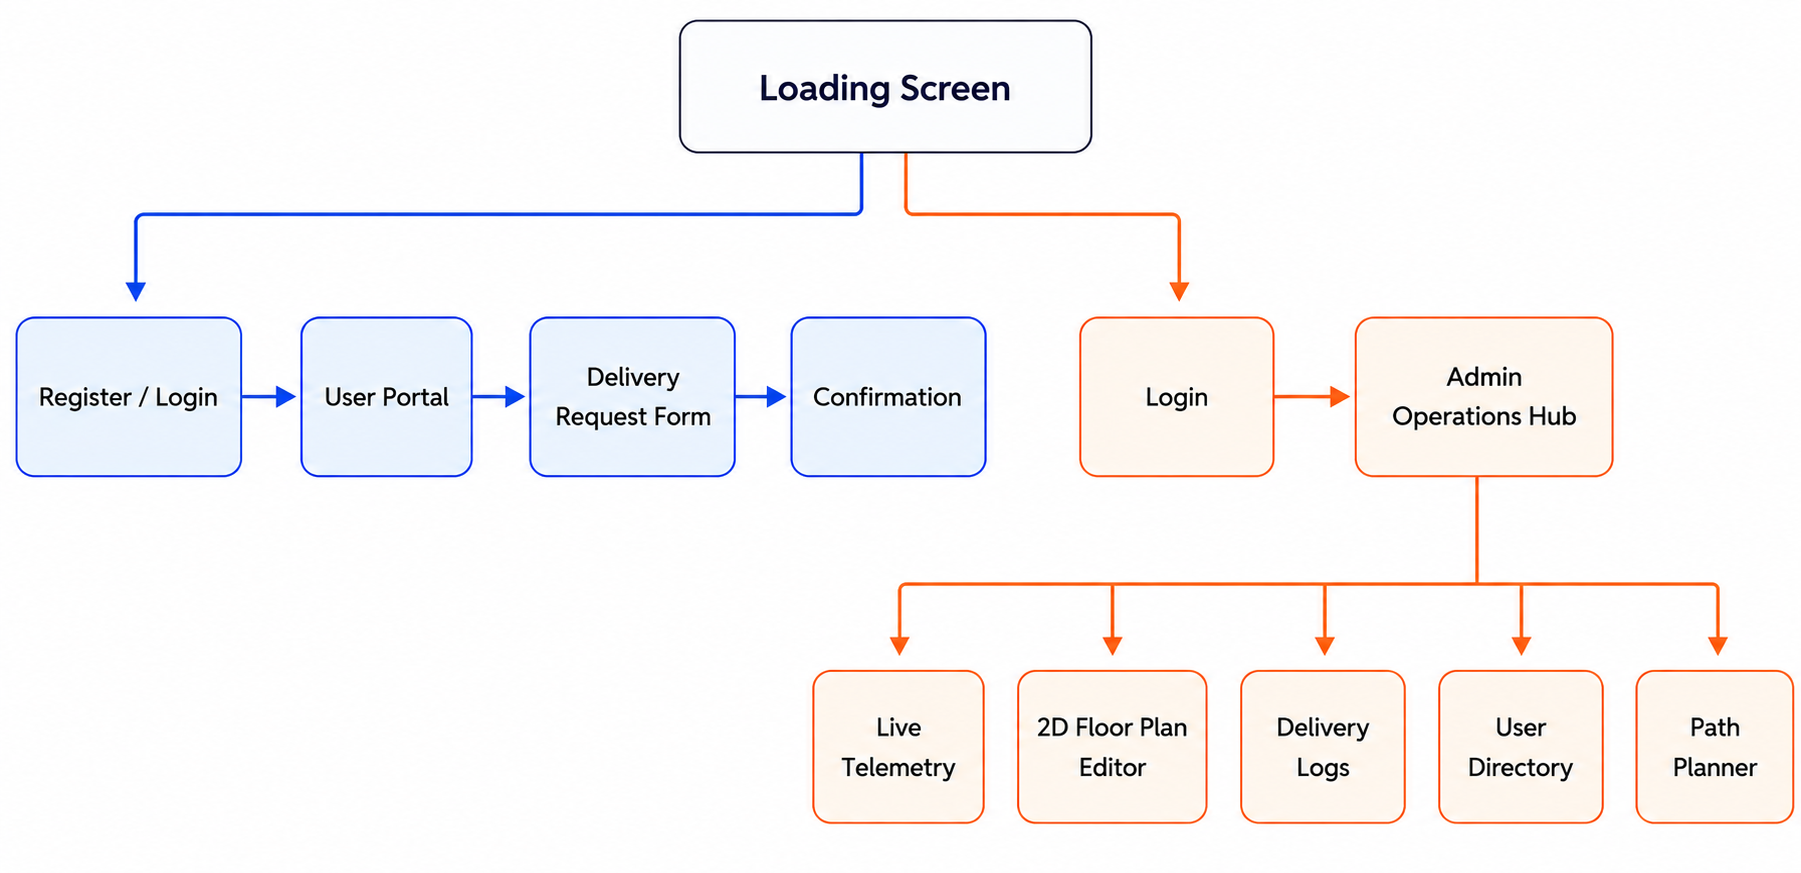
\includegraphics[width=0.9\textwidth]{app_screen_flow.png}
	\caption{Web screen flow, showing the separate user and administrator navigation paths}
	\label{fig:app_flow}
\end{figure}

\subsubsection{The Welcome Landing Screen}

With the headline \textit{``ParcelPath''} and the tagline \textit{``Autonomous indoor delivery, planned in real time''}, the application launches on a welcome landing screen that presents the platform. The user can access the login screen with just one \textbf{Get Started} action.


\subsubsection{Login and Registration}
The user is sent to either registration (complete name, email, and password) or login (registered email and password), both of which have password fields that are hidden, from the landing screen. New users can register straight from this flow, and the system ensures safe authentication by verifying email format and password strength before to submission.

\textbf{Routing based on roles.} Once the sign-in is successful, the backend identifies the user’s role and directs them to:

\begin{itemize}[noitemsep]
	\item \textbf{Users} are sent to the User’s Portal.
	\item \textbf{Administrators} are forwarded to the Admin Operations Hub.
\end{itemize}

\subsubsection{User Portal}
\label{sec:user_portal}
User Portal The main user interface is the User Portal, which shows a live status card and two necessary actions, requesting a new delivery and reviewing the delivery history record \textbf{Robot Status.} The status card represents the current state of the robot without revealing any ROS2-level information to the user. An idle robot is shown as \textit{free}, and an ongoing delivery is shown as \textit{busy} with its target room.

\textbf{Delivery Log.} The delivery history log lists each request together with its status and the date and time it was placed, so that users can track a delivery from submission through completion.

\textbf{Delivery Types.} The system supports two delivery types, distinguished by their pickup location:
\begin{itemize}[noitemsep]
	\item \textbf{Room to Room:} The robot travels from its home position to the specified pickup room to collect the parcel, then proceeds to the specified drop-off room, before finally returning to its home position.
	\item \textbf{Home to Room:} The robot's home position is itself the pickup location; the robot proceeds directly from home to the specified drop-off room and then returns.
\end{itemize}

\textbf{Requesting a New Delivery.} The Delivery Request form is centered on the same floor plan utilized to construct the Gazebo world. Rooms are represented as select blocks to enable delivery or pick-up/drop-off to be selected either from within the interactive map interface or by using its corresponding dropdown interface, to remove the need for the user to know coordinate system values. The selection live state displays a summary of rooms determined after selection. On confirmation, the backend resolves the selected rooms into their stored ROS navigation coordinates and begins the delivery process: if the robot is already free, the delivery is dispatched immediately; if the robot is busy with another delivery, the new request is queued and is automatically dispatched once the robot becomes free (or, in the case of a robot that is currently returning home, it may preempt the return trip, as described in Section~\ref{sec:fsm_design}).

\subsubsection{Admin Operations Hub (Command Center)}
\label{sec:admin_hub}

Administrators are routed to a separate Operations Hub rather than the delivery request screen. The hub presents an interactive grid layout of five independent modules, each represented by a custom line illustration that scales up slightly on hover. These modules are described below.

\textbf{Live Telemetry.} A dashboard showing the robot's real-time state. It streams the robot's $x, y$ coordinates (in metres), battery percentage, delivery queue length, and current order, and includes a live camera stream feed.

\textbf{2D Floor Plan Editor.} Allows administrators to edit and rename rooms in the building, and to update each room's coordinates so that a physical room maps to its exact pose on the map. Its design is presented in Section~\ref{sec:floor_plan_editor}.

\textbf{Path Planner.} Screen for configuring the path. It is based on an OpenStreetMap layout and offers drawing tools for workspace boundaries and circular/polygonal obstacles (static walls or furniture). It also provides solver buttons to execute A* search path calculations, cell decomposition and Particle Swarm Optimization (PSO) path smoothing. Its complete workflow is detailed in Section~3.4.3 (Phase 3: Web Platform Integration).

\textbf{Delivery Logs.} A history audit list of all deliveries with order times, status (pending, in-transit, completed) and dispatch profiles.

\textbf{User Directory.} An admin tool to list all registered users, and change their authorization roles (eg upgrade a user to Administrator) or flip their active status.

Table~\ref{tab:admin_modules} summarizes the functionality of these five modules.

\begin{table}[H]
	\centering
	\caption{Admin Operations Hub Modules}
	\label{tab:admin_modules}
	\begin{tabular}{|p{4cm}|p{10.5cm}|}
		\hline
		\textbf{Module} & \textbf{Functionality} \\
		\hline
		Live Telemetry & Streams robot position, battery percentage, queue length, current order, and live camera feed \\
		\hline
		2D Floor Plan Editor & Renames rooms and updates their navigation coordinates \\
		\hline
		Path Planner & Workspace/obstacle drawing and A*/cell-decomposition/PSO solver controls \\
		\hline
		Delivery Logs & Historical audit of all deliveries \\
		\hline
		User Directory & User role and account status management \\
		\hline
	\end{tabular}
\end{table}

\subsubsection{2D Floor Plan Editor Design}
\label{sec:floor_plan_editor}

The Floor Plan Editor is used to map each physical room to its coordinates in the robot’s navigation frame, so that the room choices provided in the delivery request form map to valid goal poses. From this screen, managers can rename rooms and adjust coordinates to keep room labels consistent with the actual facility. Each room entry is divided into two separate groups of fields deliberately: (i) \emph{visual layout} fields (bounding-box width/height and on-map position, edited as percentage sliders) that only control the room's on-screen drawing, and (ii) \emph{ROS navigation} fields ($x$, $y$, $\theta$) that control the robot's real goal pose. Table~\ref{tab:room_fields} illustrates this division, which enables the on-screen floor plan to be modified for visual clarity without risking accidental changes to the robot's calibrated delivery points.
\begin{table}[H]
	\centering
	\caption{Separation of Visual Layout and Navigation Fields in the Room Editor}
	\label{tab:room_fields}
	\begin{tabular}{|p{3.2cm}|p{4.5cm}|p{5.5cm}|}
		\hline
		\textbf{Field Group} & \textbf{Fields} & \textbf{Effect} \\
		\hline
		Visual Layout & label\_x, label\_y, region\_width, region\_height & Controls only how the room block is drawn on the floor plan (display-only) \\
		\hline
		ROS Navigation & x, y, theta & Defines the actual goal pose sent to Nav2 for that room \\
		\hline
	\end{tabular}
\end{table}

\subsubsection{Backend Server Development}

The backend server is implemented using the Python Flask framework and functions as the central coordination layer between the database, the path-planning algorithms, the web frontend and the ROS2 robotic stack. We use Flask routes to serve HTTP requests for map data, obstacle configuration, delivery management, robot telemetry, and user authentication and account management.

Table~\ref{tab:backend_files} summarizes the main backend files and their responsibilities.
\begin{longtable}{|p{0.8cm}|p{4.5cm}|p{8cm}|}
	\caption{Backend Files and Responsibilities}
	\label{tab:backend_files}\\
	
	\hline
	\textbf{Sr. No} & \textbf{File Name} & \textbf{Functionality Description} \\
	\hline
	\endfirsthead
	
	\hline
	\textbf{Sr. No} & \textbf{File Name} & \textbf{Functionality Description} \\
	\hline
	\endhead
	
	\hline
	\multicolumn{3}{|r|}{\textit{Continued on next page}} \\
	\hline
	\endfoot
	
	\hline
	\endlastfoot
	
	1 & server.py & Flask application entry point; defines REST API routes and coordinates all backend modules. \\
	\hline
	
	2 & models.py & Defines the database schema (User, Room, Delivery, Order, RobotState) using SQLAlchemy ORM. \\
	\hline
	
	3 & robot\_service.py & Implements the robot Finite State Machine (FSM) and manages ROS2 communication through rosbridge. \\
	\hline
	
	4 & astar\_modified.py & Implements the Improved A* path planning algorithm with obstacle inflation and path pruning. \\
	\hline
	
	5 & PSO\_path\_smothing.py / PSO\_implimentation.py & Implements Particle Swarm Optimization (PSO)-based path smoothing and cubic spline interpolation. \\
	\hline
	
\end{longtable}
The backend server does three main things:
\begin{itemize}[noitemsep]
	\item Accepts JSON data for map, obstacle, and delivery request
	\item Performs the selected path-planning pipeline and outputs computed trajectories
	\item Manages the robot's delivery Finite State Machine and sends navigation goals to ROS2
\end{itemize}

\subsubsection{Database Design}
\label{sec:db_design}

The system uses a relational SQLite database, through the SQLAlchemy ORM. Table~\ref{tab:db_schema} summarizes the core tables.

\begin{table}[H]
	\centering
	\caption{Core Database Tables}
	\label{tab:db_schema}
	\begin{tabular}{|p{2.5cm}|p{5cm}|p{6cm}|}
		\hline
		\textbf{Table} & \textbf{Key Fields} & \textbf{Purpose} \\
		\hline
		users & id, name, email, role & Stores login credentials and role-based access (admin/user) \\
		\hline
		rooms & id, name, x, y, theta, is\_robot\_home & Stores real-world coordinates of delivery locations \\
		\hline
		deliveries & id, sender\_id, recipient\_room\_id, status, scheduled\_at & Tracks the lifecycle of a delivery request from submission to completion \\
		\hline
		orders & id, type, pickup\_room, dropoff\_room, status & Low-level FSM task queue derived from deliveries \\
		\hline
		robot\_state & id, current\_status, x, y, battery\_level & Singleton table holding the robot's live FSM state, coordinates, and battery percentage \\
		\hline
	\end{tabular}
\end{table}

\subsubsection{Finite State Machine (FSM) Design}
\label{sec:fsm_design}

The delivery behaviour of the robot is controlled by a Finite State Machine implemented in the back-end and the current state is persisted to the robot state record described in Section~\ref{sec:db_design}. The FSM has four states: \textbf{free} (idle, parked at the home room), \textbf{en\_route\_to\_pickup} (moving to pick up a parcel for room-to-room deliveries), \textbf{en\_route\_to\_dropoff} (moving to the destination room), and \textbf{returning} (navigating back to home room after a completed delivery).

Transitions are triggered either by new delivery requests being written to the database or by success/failure callbacks from the ROS2 Nav2 action client. The complete state transition diagram is presented in Figure~\ref{fig:fsm}, and the transition logic is summarized in Table~\ref{tab:fsm_transitions}. The pickup and drop-off transitions are maintained on separate rows to correspond with the Room-to-Room and Home-to-Room delivery types described in Section~\ref{sec:user_portal}.

\begin{figure}[H]
	\centering
	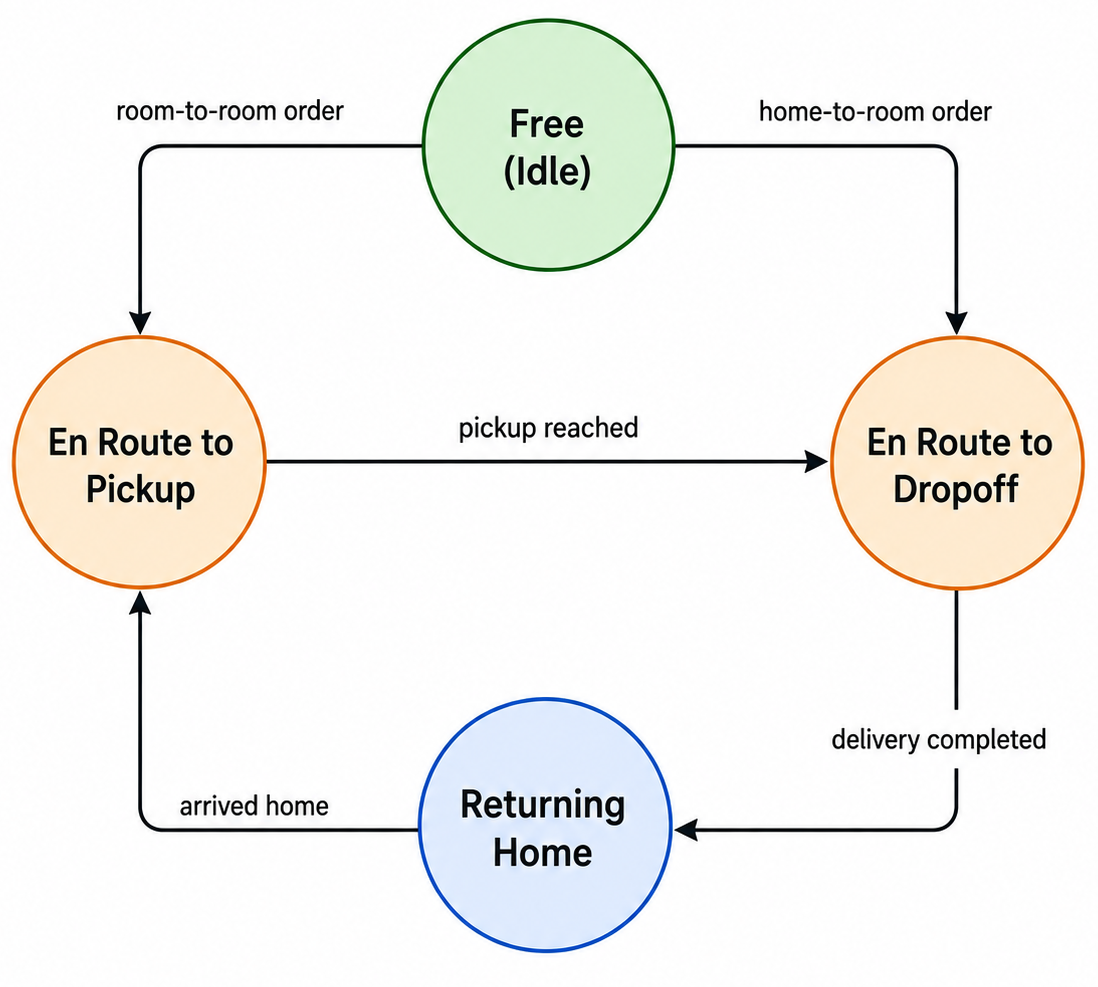
\includegraphics[width=0.6\textwidth]{fsm.png}
	\caption{Robot Delivery Finite State Machine (FSM)}
	\label{fig:fsm}
\end{figure}
\begin{longtable}{|p{3.2cm}|p{3.2cm}|p{7cm}|}
	\caption{FSM State Transitions}
	\label{tab:fsm_transitions}\\
	
	\hline
	\textbf{From State} & \textbf{To State} & \textbf{Trigger} \\
	\hline
	\endfirsthead
	
	\hline
	\textbf{From State} & \textbf{To State} & \textbf{Trigger} \\
	\hline
	\endhead
	
	\hline
	\multicolumn{3}{|r|}{\textit{Continued on next page}} \\
	\hline
	\endfoot
	
	\hline
	\endlastfoot
	
	free & en\_route\_to\_pickup & A new Room-to-Room order is dispatched; the robot must first travel to the pickup room. \\
	\hline
	
	free & en\_route\_to\_dropoff & A new Home-to-Room order is dispatched; the robot proceeds directly to the drop-off room. \\
	\hline
	
	en\_route\_to\_pickup & en\_route\_to\_dropoff & Robot reaches the pickup room (Nav2 goal succeeds). \\
	\hline
	
	en\_route\_to\_dropoff & returning & Robot reaches the destination room and the delivery is marked complete. \\
	\hline
	
	returning & free & Robot reaches the home room; the FSM checks for any queued orders. \\
	\hline
	
	returning & en\_route\_to\_pickup & A new Room-to-Room order arrives while returning. The current home-navigation goal is cancelled, and the robot is redirected to the pickup room. \\
	\hline
	
	returning & en\_route\_to\_dropoff & A new Home-to-Room order arrives while returning. The current home-navigation goal is cancelled, and the robot is redirected to the drop-off room. \\
	\hline
	
\end{longtable}
The preemption mechanism enables the robot to be redirected mid-return to a new delivery, without having to complete the trip home first, thus increasing the overall delivery throughput. It also implements the queuing behaviour exposed to the users on the User Portal (Section~\ref{sec:user_portal}): a request submitted while the robot is busy is simply stored as a pending order and automatically picked up by this same transition logic as soon as the robot becomes free.


\subsubsection{Backend-to-ROS2 Communication}

The Flask backend communicates with the ROS2 stack asynchronously via WebSockets, so there is no need to run ROS2 nodes inside the Flask process. A rosbridge\_websocket server (rosbridge\_suite) is run on port 9090 and the backend connects to it as a client via the roslibpy library. The communication path is shown in Figure~\ref{fig:ros_bridge}.

\begin{figure}[H]
	\centering
	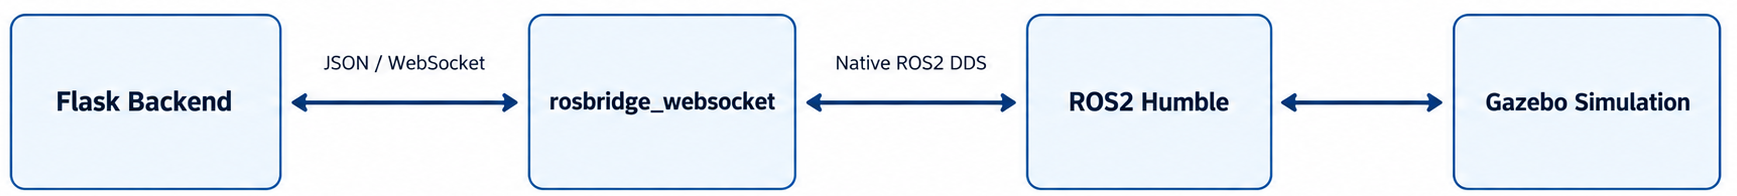
\includegraphics[width=0.8\textwidth]{ros2 bridge architecture.png}
	\caption{Backend-to-ROS2 Communication Architecture via rosbridge}
	\label{fig:ros_bridge}
\end{figure}

Table~\ref{tab:ros2_topics} summarizes the key ROS2 interfaces used in this communication. The Interface column indicates whether the channel is a Topic or an Action, and the Data Type column gives the specific ROS2 message or action type carried on that channel.

\begin{table}[H]
	\centering
	\caption{ROS2 Topics, Services, and Actions Used}
	\label{tab:ros2_topics}
	\begin{tabular}{|p{3cm}|p{2.3cm}|p{8.7cm}|}
		\hline
		\textbf{Channel} & \textbf{Interface} & \textbf{Role} \\
		\hline
		/navigate\_to\_pose & Action & Receives navigation goals from the backend FSM \\
		\hline
		/amcl\_pose & Topic & Publishes robot pose; read by backend to update telemetry \\
		\hline
		/plan & Topic & Publishes the active global trajectory; read by backend for display \\
		\hline
		/cmd\_vel & Topic & Velocity commands from the Nav2/MPPI controller to the simulated robot \\
		\hline
		/scan & Topic & Simulated LiDAR data for localization and costmaps \\
		\hline
		/camera/image\_raw & Topic & Camera stream, relayed to the web interface's Live Telemetry module \\
		\hline
		/battery\_state (simulated) & Topic & Simulated battery telemetry, relayed to the robot state record and displayed as a percentage in the Live Telemetry module and User Portal status card \\
		\hline
	\end{tabular}
\end{table}



\section{Phase 5: ROS2 \& Gazebo Setup}
\label{sec:phase5_ros2_gazebo}

In this section, the virtual machine, the operating system, the ROS2 distribution, the Gazebo simulator and the TurtleBot3 Waffle robot model are presented. This project did not need any physical hardware, as it is entirely simulation based where the entire navigation stack has been developed and tested in this virtual environment.


\subsection{Virtual Machine and Ubuntu Setup}
\label{subsec:vm_ubuntu_setup}

ROS2 and Gazebo are Linux native, so a Linux virtual machine was built on top of the host operating system using \textbf{Oracle VirtualBox}. The virtual machine was set up with at least two processing cores, 4 GB RAM and network connectivity to download packages. The ROS2 Humble distribution is officially supported on the platform Ubuntu 22.04 LTS \textbf(Jammy Jellyfish), which was installed as the guest operating system. System packages were updated after the installation to be compatible with software that would be added later.

\subsection{Gazebo 11 Classic Installation} \label{subsec:gazebo_install} \textbf{Gazebo Classic 11} was selected as the physics simulation platform, because it is the version officially coupled with ROS2 Humble via the ROS-Gazebo bridge packages. 
The Gazebo simulator and its ROS2 integration packages were installed together and the installation was verified by opening Gazebo directly to verify that it opened correctly. \subsection{TurtleBot3 Packages Installation} \label{subsec:turtlebot3_install} The simulated robot platform used was the \textbf{TurtleBot3 Waffle} robot model. All the TurtleBot3 packages were installed using the ROS2 package manager and the robot model was configured to Waffle by setting the corresponding environment variable, which was also saved permanently so it persists in the following terminal sessions.
 \subsection{ROS2 Workspace Creation} \label{subsec:ros2_workspace} All the custom packages and nodes developed for this project were maintained in a dedicated ROS2 workspace. The workspace had some custom elements such as the MPC controller node, the trajectory publisher and the custom world files. The workspace was built with ROS2’s build tool and its setup file was sourced (and added to the shell startup file, after the ROS2 Humble source line) so that all custom packages are available in addition to the basic ROS2 installation in every new terminal session.
 \subsection{World Creation} \label{subsec:gazebo_world_creation} A custom Gazebo world was developed to mimic a realistic indoor environment for testing the proposed autonomous delivery system. The environment is composed of 4 rooms linked by a central hallway, offering a mix of open spaces and narrow passages to challenge the robot’s navigation in various scenarios. Each room was furnished with different Gazebo models to emulate an indoor facility in the real world (desks, chairs, sofas, cabinets, tables, waiting areas, and other indoor fixtures). One room was dedicated as a \textbf{robot room}, which was the robot's starting place before it performed delivery tasks.Variation in furniture placement and room layouts creates a realistic environment with static obstacles as well as narrow passages to navigate through. To test the ability of the robot to work in dynamic environments, a model of a walking person was added to the simulation as a moving obstacle. This dynamic obstacle with unpredictable motion is used to test the navigation system for real-time detection, avoidance and path replanning. To launch the whole simulation environment with the TurtleBot3 Waffle robot, a dedicated ROS~2 launch file was employed. The TurtleBot3 Waffle robot provides a realistic testbed for autonomous indoor navigation and delivery experiments.

\subsubsection*{Room Coordinate Mapping}

Within each room, a known position was to be chosen as a pickup or drop-off point in the ParcelPath web interface (Phase 4) in the simulated environment. To locate these positions, a reference point was manually defined at the desired delivery location in each room of the Gazebo world. The corresponding $(x,y)$ coordinates of the selected point were then obtained directly from the \textit{Property} panel of Gazebo, which displays the pose of the selected object in the world reference frame. This procedure was performed for each room, producing a fixed set of coordinates which were then registered in the 2D Floor Plan Editor as valid navigation goals.

\begin{figure}[H]
	\centering
	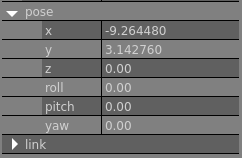
\includegraphics[width=0.4\textwidth]{coor.png}
	\caption{Gazebo Property panel displaying the world coordinates $(x,y)$ }
	\label{fig:gazebo_coordinates}
\end{figure}

The robot's home position, called the \textbf{Robo Room}, was intentionally placed near the world origin at approximately $(0,0)$ to facilitate initialization and navigation. Table~\ref{tab:room_coordinates} lists the recorded coordinates for all rooms in the simulated environment.

\begin{table}[H]
	\centering
	\caption{Registered Room Coordinates}
	\label{tab:room_coordinates}
	\begin{tabular}{|c|p{3cm}|p{3cm}|p{3cm}|}
		\hline
		\textbf{ID} & \textbf{Name} & \textbf{X Coordinate} & \textbf{Y Coordinate} \\
		\hline
		1 & Room 1 & -14.6662 & 2.28722 \\
		\hline
		2 & Room 2 & -9.26448 & 3.14276 \\
		\hline
		3 & Room 3 & -14.9200 & -1.62217 \\
		\hline
		4 & Room 4 & -9.00083 & -2.43645 \\
		\hline
		5 & Robo Room & 0.0000 & 0.0000 \\
		\hline
	\end{tabular}
\end{table}

These recorded coordinates are used to map the actual rooms in the Gazebo environment to the corresponding delivery locations in the ParcelPath web interface .

\subsection{Environment Configuration Summary}
\label{subsec:gazebo_config_summary}

Table~\ref{tab:gazebo_configuration_p5} summarizes the complete simulation environment configuration.

\begin{table}[H]
	\centering
	\caption{Gazebo Simulation Environment Configuration}
	\label{tab:gazebo_configuration_p5}
	\begin{tabular}{|p{3.5cm}|p{10cm}|}
		\hline
		\textbf{Component} & \textbf{Description} \\
		\hline
		Virtualization & Oracle VirtualBox \\
		\hline
		Operating System & Ubuntu 22.04 LTS (Jammy Jellyfish) \\
		\hline
		ROS Distribution & ROS2 Humble Hawksbill \\
		\hline
		Simulation Platform & Gazebo 11 Classic \\
		\hline
		Robot Model & TurtleBot3 Waffle \\
		\hline
		Environment Design & Four rooms with one Robo room connected by a hallway, with a dynamic walking-person obstacle \\
		\hline
		Visualization & RViz2 for real-time monitoring \\
		\hline
		Physics Engine & ODE (Open Dynamics Engine) \\
		\hline
	\end{tabular}
\end{table}


\subsection{Navigation Reliability Assessment in Dynamic Environments}

The time of execution of both A* and dynamic planning algorithms in order to compare their efficiencies in terms of algorithms to the varied map complexities.

\begin{itemize}[noitemsep]
	\item Path replanning capability
	\item Obstacle avoidance consistency
	\item Robot stability under dynamic disturbances
	\item Controller response to environmental changes
\end{itemize}


The test establishes that the navigation structure works well in the real world. Table~\ref{tab:performance_metrics} lists the performance metrics used in the course of the navigation analysis, including quality of path, smoothness, tracking accuracy, computational efficiency, and reliability, which allows performing a full assessment of the system.
% Table 3.1
\begin{table}[H]
	\centering
	\caption{Performance Evaluation Metrics Used for Navigation Analysis}
	\label{tab:performance_metrics}
	\begin{tabular}{|p{3.5cm}|p{3.5cm}|p{5.5cm}|}
		\hline
		\textbf{Evaluation Category} & \textbf{Metric} & \textbf{Description} \\
		\hline
		Path Quality & Path Length & Total distance traveled by robot \\
		\hline
		Path Smoothness & Curvature Continuity & Measures directional consistency \\
		\hline
		Tracking Accuracy & Tracking Error & Deviation from reference trajectory \\
		\hline
		Computational Efficiency & Algorithm Execution Time & Time required for path planning and optimization \\
		\hline
		Reliability & Obstacle Avoidance Success Rate & Ability to avoid static and dynamic obstacles \\
		\hline
	\end{tabular}
\end{table}

% ============================================================
% UPDATED REPLACEMENT BLOCK for chapter3.tex (v3)
% Covers: Phase 2 (Web Interface) through System Integration and Testing
% Paste this in place of the corresponding existing block.
% Uses the same \subsection / \subsubsection formatting already
% defined in main.tex — no formatting commands changed.
%
% CHANGES IN THIS VERSION:
%   - Admin Operations Hub modules (previously an A/B/C/D/E
%     description list) are now individual bold lead-in paragraphs
%     ("Live Telemetry.", "2D Floor Plan Editor.", etc.), matching
%     the style already used in the User Portal subsection — no
%     more lettered list.
%   - Removed \texttt{CustomPainter} styling from the prose; the
%     Admin Hub intro now describes the hover illustrations without
%     naming the specific Flutter widget class.
%   - "Admin Operations Hub Modules and Source Files" table is now
%     a 2-column table (Module, Functionality): the Source File
%     column and the A./B./C. letter prefixes have been removed.
%   - FSM State Transitions table: rows that previously combined
%     two destination states in one cell (e.g. "en_route_to_pickup
%     / en_route_to_dropoff") are now split into separate rows, one
%     transition per row, with the Room-to-Room vs Home-to-Room
%     distinction stated explicitly in the trigger column.
%   - ROS2 Topics table: fixed an inconsistent message-type string
%     (the /amcl_pose row was missing "/msg/", unlike every other
%     row) and relabelled the columns (Interface / Data Type) so
%     the Type and Message/Action columns no longer read as
%     duplicates of each other.
% ============================================================

\section{Phase 6: MPPI Navigation}
\label{sec:phase7_mppi}

While the MPC controller (Phase 3) tracks the smoothed global path under nominal conditions, it relies on a fixed cost formulation and struggles to react quickly to unexpected, close-range disturbances such as a moving obstacle suddenly entering the robot's path. To address this, \textbf{Model Predictive Path Integral (MPPI) control} was introduced as a local planner, working alongside the global planning pipeline (Phases 1--2) to detect and avoid dynamic obstacles particularly a person walking through the robot's path in real time.

\subsection{What is MPPI}
\label{subsec:mppi_overview}

Model Predictive Path Integral (MPPI) is a sampling-based model predictive control method. Unlike traditional MPC, which solves a constrained optimization problem analytically or through gradient-based solvers, MPPI works by randomly generating many possible future control sequences rollouts, simulating the outcome of each one using the robot's motion model, scoring each rollout with a cost function, and then combining them into a single weighted-average control command.

This sampling-based approach has several practical advantages for local, reactive navigation:

\begin{itemize}[noitemsep]
	\item It does not require the cost function or motion model to be smooth or differentiable, so arbitrarily complex costs (e.g. sharp obstacle penalties) can be used directly.
	\item It naturally handles nonlinear dynamics and non-convex obstacle constraints, which are difficult for gradient-based MPC to optimize reliably.
	\item It can be updated at high frequency, making it well suited for reacting to sudden, dynamic obstacles such as a walking person crossing the robot's path.
\end{itemize}

For these reasons, MPPI was integrated as the \textbf{local planner}, responsible for short-horizon, reactive obstacle avoidance, while the global planner (A* with PSO smoothing) remains responsible for long-horizon route planning across the full environment.

\subsection{Local Planning with MPPI}
\label{subsec:mppi_local_planning}

At every control cycle, the MPPI local planner performs the following steps:

\begin{enumerate}[noitemsep]
	\item \textbf{Sample} a large number ($K$) of candidate control sequences, each consisting of a short sequence of linear and angular velocity commands, by perturbing a nominal control sequence with random noise.
	\item \textbf{Simulate (rollout)} each candidate sequence forward through the robot's kinematic model over a short prediction horizon, producing $K$ candidate future trajectories.
	\item \textbf{Evaluate} each candidate trajectory using a cost function that penalizes deviation from the local reference path, proximity to obstacles (including the dynamic walking-person obstacle), and excessive control effort.
	\item \textbf{Weight} each candidate trajectory using a soft-min (exponential) weighting based on its cost 
	\item \textbf{Combine} all weighted candidate control sequences into a single optimal control sequence.
	\item \textbf{Apply} only the first control command of this combined sequence to the robot, then repeat the entire process at the next control cycle (receding horizon, similar to Phase 3).
\end{enumerate}

Because MPPI operates over a short horizon and reacts directly to real-time sensor data (LiDAR-detected obstacles), it complements the global planner by handling situations the global plan could not anticipate, such as a person walking into the corridor after the global path was already computed.

\subsection{Mathematical Formulation}
\label{subsec:mppi_math}

Given a nominal control sequence $U = (u_0, u_1, \dots, u_{N-1})$, MPPI generates $K$ perturbed control sequences:

\begin{equation}
	u_k^{(i)} = u_k + \epsilon_k^{(i)}, \qquad i = 1, \dots, K
	\label{eq:mppi_perturbation}
\end{equation}

where $\epsilon_k^{(i)} \sim \mathcal{N}(0, \Sigma)$ is Gaussian noise sampled independently for each rollout $i$ and each time step $k$, with covariance $\Sigma$.

Each rollout $i$ is assigned a cost $S^{(i)}$, accumulated over the horizon:

\begin{equation}
	S^{(i)} = \sum_{k=0}^{N-1} c(x_k^{(i)}, u_k^{(i)}) + c_{terminal}(x_N^{(i)})
	\label{eq:mppi_cost}
\end{equation}

where $c(x_k, u_k)$ is the running cost (tracking error, obstacle penalty, control effort) and $c_{terminal}$ penalizes the final predicted state.

The optimal control update is computed as a cost-weighted average over all rollouts:

\begin{equation}
	u_k^{*} = u_k + \frac{\sum_{i=1}^{K} \exp\left(-\frac{1}{\lambda} S^{(i)}\right) \epsilon_k^{(i)}}{\sum_{i=1}^{K} \exp\left(-\frac{1}{\lambda} S^{(i)}\right)}
	\label{eq:mppi_update}
\end{equation}

where $\lambda$ is a temperature parameter which can be used to trade-off the preference of the lowest cost rollouts and the higher cost rollouts: a smaller $\lambda$ gives more weight to the lowest cost rollouts, while a larger $\lambda$ gives a more averaged result.
\subsection{Parameters}
\label{subsec:mppi_parameters}
Table~\ref{tab:mppi_parameters} summarizes the MPPI local planner configuration used in this project.

\begin{longtable}{|p{5cm}|p{2.5cm}|p{6cm}|}
	\caption{MPPI Local Planner Parameters}
	\label{tab:mppi_parameters} \\
	
	\hline
	\textbf{Parameter} & \textbf{Symbol} & \textbf{Value} \\
	\hline
	\endfirsthead
	
	\hline
	\textbf{Parameter} & \textbf{Symbol} & \textbf{Value} \\
	\hline
	\endhead
	
	\hline
	\multicolumn{3}{r}{\textit{Continued on next page}} \\
	\hline
	\endfoot
	
	\hline
	\endlastfoot
	
	Number of Samples (Rollouts) &
	$K$ &
	1000 \\
	\hline
	
	Prediction Horizon &
	$N$ &
	30 steps \\
	\hline
	
	Sampling Time &
	$\Delta t$ &
	0.05 seconds \\
	\hline
	
	Temperature Parameter &
	$\lambda$ &
	1.0 \\
	\hline
	
	Control Noise Standard Deviation (linear velocity) &
	$\sigma_v$ &
	0.2 m/s \\
	\hline
	
	Control Noise Standard Deviation (angular velocity) &
	$\sigma_\omega$ &
	0.4 rad/s \\
	\hline
	
	Linear Velocity Limits &
	$v$ &
	$v \in [0,0.26]$ m/s \\
	\hline
	
	Angular Velocity Limits &
	$\omega$ &
	$\omega \in [-1.9,1.9]$ rad/s \\
	\hline
	
	Obstacle Cost Weight &
	-- &
	50.0 \\
	\hline
	
	Path Tracking Cost Weight &
	-- &
	10.0 \\
	\hline
	
	Minimum Safe Obstacle Distance &
	-- &
	0.35 m \\
	\hline
	
\end{longtable}
1000 sample paths provide the controller with sufficient options to choose the most secure path without exceeding the maximum processing time per step. The low value of temperature ($\lambda=1.0$) makes the robot commit strongly to the single best path it finds, rather than blend it with riskier options -- so it reacts quickly and decisively when the person gets close. Finally, the obstacle avoidance weight (50.0) is set much higher than the path following weight (10.0) so the robot is happy to deviate from the original path to avoid a collision rather than strictly following its route.

\subsection{Integration with the Global Planner}
\label{subsec:mppi_integration}

MPPI operates as a local planning layer on top of the global path produced in Phases 1 and 2, forming a two-tier navigation architecture:

\begin{itemize}[noitemsep]
	\item The \textbf{global planner} (Improved A* with PSO smoothing) computes a long-horizon, obstacle-free path across the entire known map, based on the static occupancy grid.
	\item The \textbf{local planner} (MPPI) continuously tracks a short rolling section of this global path, while reacting in real time to LiDAR sensor data that may reveal dynamic obstacles  most notably the \textbf{walking person} present in the Gazebo simulation world (Phase 5) that are not represented in the original static map.
\end{itemize}

At each control cycle, the local reference segment for MPPI is extracted from the nearest upcoming portion of the global path. Under normal conditions, with no dynamic obstacles nearby, MPPI closely tracks this reference segment, producing motion very similar to the underlying MPC tracking behavior (Phase 3). However, when the walking-person obstacle moves into or near the robot's planned path, the obstacle cost term in the MPPI cost function (Equation~\ref{eq:mppi_cost}) sharply penalizes any rollout that passes too close to the obstacle's detected position. Since MPPI evaluates a large number of randomly sampled trajectories at every cycle, it naturally identifies alternative rollouts that steer around the obstacle while still making progress toward the local goal, and the weighted combination of these low-cost rollouts produces a smooth avoidance maneuver.

Once the dynamic obstacle is out of the way of the robot, the obstacle cost term is no longer dominant and the path tracking cost term pulls the robot back to the original global path. This multi-layered design takes advantage of the benefits of both planners: the global planner ensures that the robot has always an efficient and complete path to the goal, while the local MPPI planner ensures safe, reactive behavior in the presence of unpredictable, real-time disturbances, like a person walking in the corridor that the global planner cannot anticipate in advance.



\section{Phase 7: Rviz setting }

\subsection{RViz Visualization Configuration}

For visualization of the custom navigation stack outputs during simulation, RViz2 was configured with dedicated Path displays for the raw global planner output and the optimized trajectory for control. Figure~\ref{fig:rviz_settings}
shows the corresponding display settings.

The raw global path generated by the Improved A* planner is subscribed from the \textit{/plan} topic and visualized in green Lines style (RGB: 25, 255, 0).
The pruned and PSO-smoothed trajectory from the \textit{/plan\_smoothed} topic is plotted separately with blue Lines style (RGB: 0, 170, 255). For both displays the buffer length is 1, thus only the most recently published path is displayed at any time, instead of the accumulated older paths from previous planning cycles.
This configuration allows for real time visual comparison of the raw A* output and the PSO-smoothed path within the same scene, allowing for direct observation of the effect of the pruning and smoothing stages on the quality of the path.
The Model Predictive Controller subscribes to the smoothed path on \textit{/plan\_smoothed} and uses it as the reference trajectory to generate the velocity commands that drive the robot’s motion.

\begin{figure}[h]
	\centering
	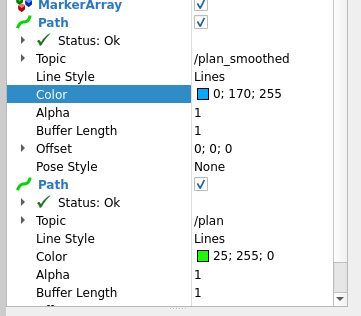
\includegraphics[width=0.5\textwidth]{setting.png}
	\caption{RViz configuration showing the raw A* global path
		and the PSO-smoothed path used as	the reference trajectory for the MPC controller.}
	\label{fig:rviz_settings}
\end{figure}

\section{Design of the Project Hardware}

The current project is fully a simulation project and does not need any physical hardware design and development. The autonomous navigation system, such as the modeling of the robot, the process of sensor integration, the creation of the environment, the execution of the path planning and the tracking of the trajectory are all implemented and tested in Gazebo simulation environment with ROS2 with Jazzy. The TurtleBot3 Waffle robot example is the virtual hardware platform and all specifications, sensors, and motion dynamic specifications are defined by the parameters in the simulation process, which ensures the whole system development and testing process are done in a fully virtual environment without the necessity of having any physical hardware components.

\section{Details of Final Working Prototype}
\label{sec:final_prototype}

The final working prototype integrates all six development phases described in
the preceding sections into a single, end-to-end simulated delivery pipeline. The
complete system is brought online through a fixed startup sequence executed across
multiple terminals, after which the robot is able to autonomously accept, plan, and
execute delivery tasks issued from the web interface.
The prototype requires five independent processes to be launched in sequence, each
in its own terminal, before the system becomes fully operational:
\begin{enumerate}
	\item \textbf{Gazebo Simulation:} The custom indoor world,
	together with the TurtleBot3 Waffle robot model, is launched using the
	project's ROS 2 launch file. This initializes the physics simulation,
	the robot's sensors (LiDAR and RGB camera), and the dynamic walking-person
	obstacle.
	
	\item \textbf{RViz Visualization:} RViz2 is launched to provide real-time
	visualization of the occupancy map, the robot's localized pose, the planned
	global path, and the local MPPI-adjusted trajectory during navigation.
	
	\item \textbf{Rosbridge WebSocket Server:} The rosbridge server is started
	on port 9090 to expose the ROS 2 communication layer to the Flask backend
	by running ros2 launch rosbridge\_server rosbridge\_websocket\_launch.xml.
	This bridge is what allows the backend to publish navigation goals and
	subscribe to telemetry, pose, and battery topics over a standard WebSocket
	connection rather than requiring a native ROS 2 client.
	
	\item \textbf{Camera Streaming Server:} The web\_video\_server
	package is launched to relay the robot's RGB camera feed as an
	HTTP-accessible video stream by running ros2 run web\_video\_server
	web\_video\_server. This stream is used directly by the Live Telemetry module of the Admin Operations Hub.
	
	\item \textbf{Backend and Frontend Servers:} Finally, the Flask backend server (server.py) and the Flutter frontend (ParcelPath) are started, completing the software stack and making the web application available to the user.
\end{enumerate}
\subsection*{End-to-End Delivery Workflow}

With the prototype fully launched, a complete delivery is executed as follows:

\begin{enumerate}
	\item \textbf{Authentication.} The user logs in through the ParcelPath
	landing screen and is routed, based on their role, to either the User
	Portal or the Admin Operations Hub
	
	\item \textbf{Task Assignment.} A user creates a delivery request simply by selecting their drop-off and/or pickup room from the interactive map/room selection menu and confirms the request. The mapped/selected rooms are resolved to their programmed navigation co-ordinates, and these co-ordinates are communicated back to the backend.
	
	\item \textbf{Dispatch and Queuing.} The backend's Finite State Machine
 checks the robot's current status. If the
	robot is the delivery is dispatched immediately; otherwise,
	the request is stored as a pending order and automatically dispatched once
	the robot becomes available.
	
	\item \textbf{Path Planning.} Upon dispatching, the backend call the whole
	planning pipeline, which consists of: An Improved A* planning a collision-free trajectory on the
	grid Path pruning that get rid of unnecessary points and PSO based smoothing algorithm that generates a
	kinematically feasible trajectory in an ongoing curve.
	\item \textbf{Trajectory Tracking.} The smoothed trajectory is published
	to ROS 2 and subscribed to by the MPC controller node in RViz/Gazebo, which computes velocity commands to
	track the path while respecting the robot's kinematic and actuator
	constraints.
	
	\item \textbf{Dynamic Obstacle Avoidance.} While executing the planned
	trajectory, the MPPI local planner continuously monitors LiDAR data for unexpected obstacles, most notably the
	walking-person model in the simulation, and reactively adjusts the robot's
	short-horizon motion to avoid collisions before resuming the original path.
	
	\item \textbf{Live Monitoring.} As it’s running the robot’s position, battery life, and delivery state is broadcast back to the web application interface. Admins will also want to watch the progress of the delivery using Live Telemetry to see where the robot is in real-time, together with its live camera Feed sent over Web video service.
	\item \textbf{Completion and Return.} When the delivery is completed and the FSM reaches the drop-off room, it becomes marked as completed in the database, and the FSM changes its current state from route to dropoff to returning back towards Robo Room. If when the robot reaches home, there are no other deliveries in the delivery pipeline, then the FSM changes from returning to free and the robot stays at home doing nothing, till a new delivery request comes. But if in case of any other delivery request when the robot was on its way home to reach the Free state, then the currently pursuing home-navigation goal is cancelled, and the robot will start heading towards the pickup or the dropoff location of the new order, without completing the return journey, therefore reducing delay of new delivery.
\end{enumerate}

\begin{figure}[h]
	\centering
	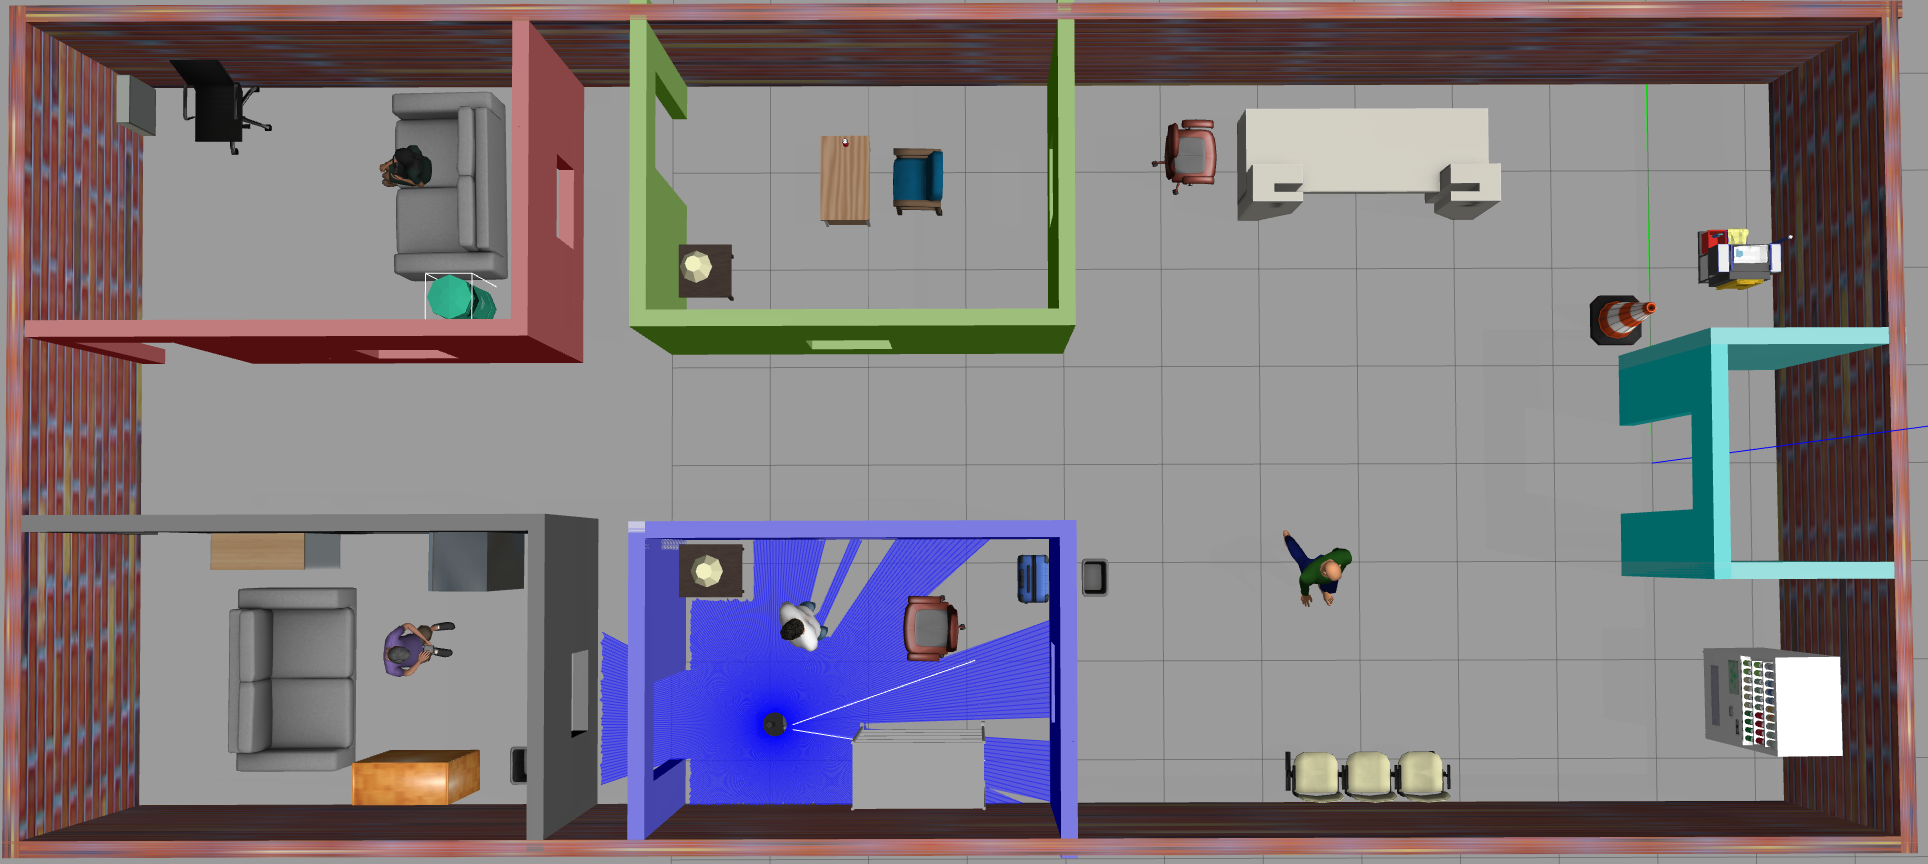
\includegraphics[width=0.75\textwidth]{gazebo_marking_robot_at_delivery_point}
	\caption{TurtleBot3 Waffle robot completing delivery task at
		the destination.}
	\label{fig:delivery_complete}
\end{figure}

This complete workflow,spanning task assignment, global path planning,
smoothing, MPC-based tracking, MPPI-based dynamic obstacle avoidance,
real-time telemetry, and FSM-driven dispatch (including mid-return
preemption for queued orders)  demonstrates that the proposed system
successfully integrates all six development phases into a functioning,
simulation-based autonomous parcel delivery prototype.
\section{Chapter Summary}
\label{sec:chapter_summary}

This chapter presented the design and implementation of the autonomous parcel
delivery system, developed through six phases: global path planning, path
optimization, controller design, web and backend development, ROS2/Gazebo
simulation setup, and MPPI-based dynamic obstacle avoidance.The Improved A* algorithm generated collision-free global paths, which were
pruned and smoothed using Particle Swarm Optimization to produce short,
feasible trajectories. A Model Predictive Controller tracked these paths whilerespecting the robot's motion constraints, and an MPPI local planner was addedto reactively avoid dynamic obstacles such as a moving person.
A web platform, ParcelPath, was built with a Flutter frontend and Flask
backend to let users request deliveries and let admins monitor the robot via
live telemetry and camera feed.A Finite State Machine handled the delivery dispatch and the queuing and preemption upon return, communicating with ROS2 via rosbridge. The entire system was tested in a custom Gazebo world with TurtleBot3 with reliable path planning, smooth trajectory tracking, and effective obstacle avoidance, all fully simulated without any physical hardware.
    \chapter{TOOLS AND TECHNIQUES}

\section{Overview}
The software tools and development platforms utilized for the planned final year project's design, implementation, simulation, and documentation are described in this chapter. The selected tools were chosen based on their industry relevance,reliability, and support for collaborative development. All these tools enabled an efficient coding, simulation, testing, and documentation process as well as managing the entire project lifecycle.


\section{Hardware Tools Used}
The proposed project is primarily software-based and simulation-oriented. No dedicated
external hardware components were required during the development and testing phases.
All activities were carried out using standard personal computing systems with adequate
processing power, memory, and storage to support software development environments
and simulation tools.

\section{ Software and Simulation Tools}
This part describes the major environment and simulation tools to be used in the implementation and testing of the navigation algorithms in the robot.

\subsection{Oracle VirtualBox}

Oracle VirtualBox~\cite{virtualbox2024} is an open-source virtualization platform that is free and also allows running multiple operating systems at the same time and without disrupting the host system. VirtualBox was used in this project to create a dedicated Ubuntu Linux virtual machine on the workstations based on Windows, therefore, providing the necessary Linux environment to develop ROS~2. VirtualBox was the base layer of the whole development architecture where all the project-specific software was installed and ran.
\begin{figure}[H]
	\centering
	
\includegraphics[width=0.3\textwidth]{vbox.png}
	\caption{Oracle VirtualBox Logo~\cite{virtualbox2024}}
	\label{fig:vbox_logo}
\end{figure}

\subsection{Ubuntu Linux}
Ubuntu Linux~\cite{ubuntu2024} is an open-source operating system that is heavily used in the research and development of robotics. The version chosen to be used in this project was Ubuntu 22.04 LTS (Jammy Jellyfish), which was chosen as the officially supported platform of ROS 2 Jazzy Jalisco; this name has ensured compatibility with all the necessary packages and libraries. As a result, Ubuntu served both as the primary development platform of all associated operations and as the command-line interface to compile ROS2 packages, dependencies, and run simulations.  

\begin{figure}[h]
	\centering
	
\includegraphics[width=0.4\textwidth]{ubuntu.jpg}
	\caption{Ubuntu Logo~\cite{ubuntu2024}}
	\label{fig:ubuntu_logo}
\end{figure}

\subsection{Visual Studio Code}
Microsoft created Visual Studio Code~\cite{vscode2024}, a lightweight yet potent source code editor. The project source code was written, edited, and debugged using it as the main development environment. Extensive extension support and smooth version control system integration are features of Visual Studio Code.
\begin{figure}[H]
	\centering
	
\includegraphics[width=0.20\textwidth]{vscode.png}
	\caption{Visual Studio Code Logo~\cite{vscode2024}}
	\label{fig:vscode_logo}
\end{figure}

\subsection{ROS 2 and Gazebo Simulation Environment}
An open-source middleware framework for creating robotic applications is called Robot Operating System~2 (ROS~2)~\cite{ros2jazzy2024}. It divides software into nodes, which are modular parts that interact with one another through action servers, services, and topics. The main basis for this project was ROS~2. The core of the system was ROS~2.

An open-source 3D robot simulator called Gazebo~\cite{gazebo2024} offers a physics-based environment for testing robotic systems prior to their implementation on actual hardware. To verify the navigation algorithms in a secure virtual setting, it was integrated with ROS~2. Based on the TurtleBot3 platform~\cite{turtlebot3doc}, the robot model had wheel encoders, a depth camera, and a simulated LiDAR. In order to test path planning, obstacle avoidance, and multi-waypoint delivery missions, custom indoor settings featuring walls, hallways, and obstacles were constructed. This eliminated the requirement to run unverified code on real hardware during development.

\begin{figure}[h]
	\centering
	
\includegraphics[width=0.3\textwidth]{ros.png}
	\caption{ROS~2 Jazzy Jalisco Logo~\cite{ros2jazzy2024}}
	\label{fig:ros2_logo}
\end{figure}

\subsection{Google Colaboratory}

A cloud platform called Google Colaboratory (Colab)~\cite{colab2024} offers a Jupyter notebook platform that enables users to develop and execute Python code in a web browser without requiring a local configuration. It provides unrestricted access to the GPU's processing capabilities, making it especially suitable for algorithm development and data analysis endeavors.

\begin{figure}[h]
	\centering
	
\includegraphics[width=0.5\textwidth]{colab.png}
	\caption{Google Colaboratory Logo~\cite{colab2024}}
	\label{fig:colab_logo}
\end{figure}

\subsection{GitHub}
GitHub~\cite{github2024} is an online platform that uses Git version control to store and manage source-code repositories.
It was used during the research in controlling the code, documenting changes and supporting interaction between members of a project. Each team member worked on separate branches, and then could combine changes through pull requests once they had been reviewed. GitHub also served as a reliable cloud backup protecting the project from data loss.
\begin{figure}[H]
	\centering
	
\includegraphics[width=0.4\textwidth]{github.png}
	\caption{GitHub Logo~\cite{github2024}}
	\label{fig:github_logo}
\end{figure}

\subsection{Flutter}

Flutter~\cite{flutter2024} is an open-source framework that Google created to create cross-platform mobile apps in the Dart programming language. It was applied in this project to create the mobile application frontend enabling the customers to make the delivery request, see the real-time location of the robot, and get the status messages. The hot reload support in Flutter allowed the development and testing of the UI quickly, and the cross-platform nature of this environment was useful in ensuring that the application is compatible with both the Android and iOS platforms without needing to maintain two separate codebases.

\begin{figure}[h!]
	\centering
	
\includegraphics[width=0.3\textwidth]{flutterjpg.jpg}
	\caption{Flutter Framework Logo~\cite{flutter2024}}
	\label{fig:flutter_logo}
\end{figure}

\subsection{Flask}

Flask~\cite{flask2024} is a lightweight Python framework that is employed in the development of web applications. It was used in this project to build up the back-end server which is responsible in dealing with the communication between the web application and the autonomous robot. The Flask server receives delivery requests using the mobile application, writes the information into the database, and dispatches the navigation instructions to the ROS 2 system.
\begin{figure}[H]
	\centering
	
\includegraphics[width=0.5\textwidth]{flask.png}
	\caption{Python Flask Backend Architecture~\cite{flask2024}}
	\label{fig:flask_logo}
\end{figure}

\subsection{Overleaf}
Overleaf~\cite{overleaf2024} is an online collaborative LaTeX editor used for writing and formatting academic documents. It was utilized in this project to create the final report in compliance with Capital University of Science and Technology's (CUST) formatting specifications. A professionally designed paper with consistent headings, captions, equations, and IEEE-style citations was created by using LaTeX through Overleaf.

\begin{figure}[h]
	\centering
	
\includegraphics[width=0.3\textwidth]{overleaf.png}
	\caption{Overleaf Logo~\cite{overleaf2024}}
	\label{fig:overleaf_logo}
\end{figure}

\section{Summary}
The software tools utilized for the project were described in this chapter. Visual Studio Code was the primary IDE for all coding operations, and Oracle VirtualBox housed the Ubuntu development environment. Gazebo offered a physics-based simulation platform for testing navigation algorithms prior to hardware deployment, while ROS~2 Jazzy served as the fundamental robotics framework. Overleaf facilitated expert report creation, GitHub preserved version control and teamwork, while Google Colab helped early algorithm prototyping and SLAM implementation. Together, they supported every stage of the project, from concept to final documentation, and each tool was chosen for a particular function.
	\chapter{PROJECT RESULTS AND EVALUATION}

The outcomes of the Autonomous Parcel Delivery System, which was created and tested throughout five stages, are presented in this chapter. From a basic Python script to a complete robotics simulation, each stage builds directly on the outcomes of the one before it. Making ensuring each part functioned well before introducing the next level of complexity was the main objective.


% ══════════════════════════════════════════════════════════════════════════════

\section{Presentation of the Findings}

The outcomes of the Autonomous Parcel Delivery System's development and testing are shown in this section. The result of the project is fully implemented in software and the emphasis is placed on the performance of the path planning component, the motion control component and the web interface, all of which were tested and evaluated in different scenarios.


\section{Phase 1: Path Planning in VS Code}

In the first phase the path planning logic was written and implemented in a Python environment using Visual Studio Code. This was intentionally done by keeping things simple at first, any bugs in the algorithm could be caught and fixed without the added complexity of ROS 2 or hardware.Everything was done in parts and then integrated together The planning process was broken into four steps.

% ─── Step 1 ──────────────────────────────────────────────────────────────────
\subsection{Step 1: Exploring the Map with A*}

The first task was to find a route through the map. The Improved A* (IA*) algorithm was used for this purpose. It works by starting at the robot's position and expanding outward, checking which directions lead closer to the goal while avoiding obstacles.

The red crosses in the figure \ref{fig:astar} represent every grid cell the algorithm checked before finding the solution. The best thing to observe is the manner in which the search went around the barrier in the middle of the map.The fact that the A-star managed to navigate around the obstacle is a confirmation that the heuristic functionality is properly functioning and leading the search in a reasonable direction.

\begin{figure}[H]
	\centering
	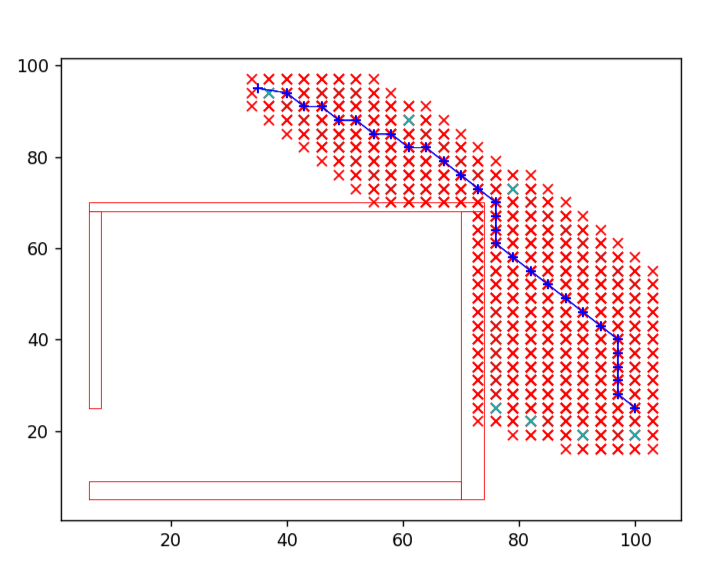
\includegraphics[width=0.6\textwidth]{A(star).png}
	\caption{A* node expansion showing exploration process}
	\label{fig:astar}
\end{figure}

The figure shows every cell visited during the search process, marked with red crosses. The algorithm successfully avoids the U-shaped trap in the center and reaches the goal, indicated by the blue star. This demonstrates the effectiveness of the heuristic function in guiding the search toward the goal while navigating around complex obstacles.

% ─── Step 2 ──────────────────────────────────────────────────────────────────
\subsection{Step 2: Generating the Raw Path}

Once the goal was found, the algorithm traced back through its steps to draw the route it had taken. This is called the raw path, shown as a green line in the figure.

Although this is technically right it takes over all the challenges and links the starting point to.
complete yet it is very rough. It consists of diagonal and right angle steps that are short.
follow the grid pattern of the map. A real robot cannot move in such a way: those sharp.
corners would make it come to a halt and turn and then come to a halt again each turn. So although
this is the step that the planner was sure that he has walked the correct path.
\begin{figure}[H]
	\centering
	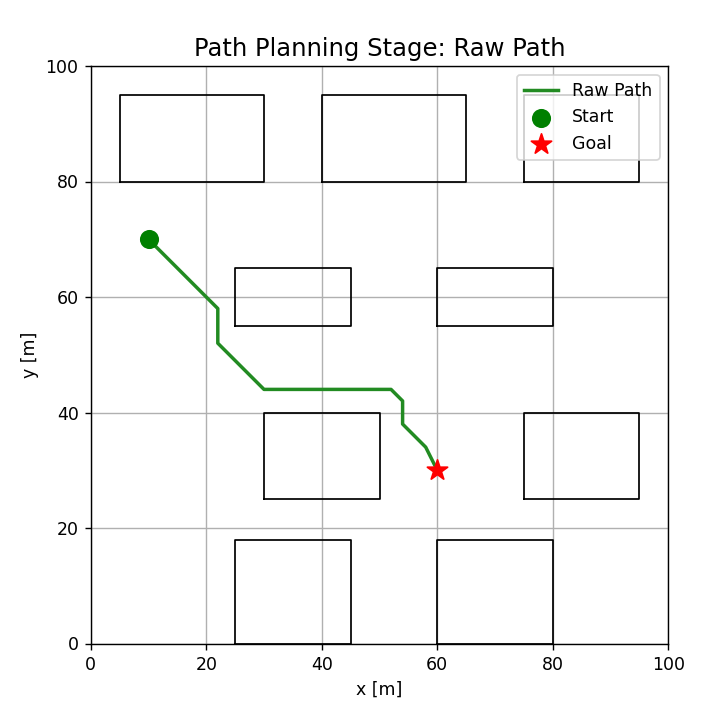
\includegraphics[width=0.7\textwidth]{Raw path.png}
	\caption{Raw path generated by A* algorithm}
	\label{fig:raw}
\end{figure}

The green line represents the raw path output from the A* algorithm. While collision free and connecting start to goal, the path follows the rigid grid structure, producing jagged movements with sharp corners. These movements are impractical for a real robot to execute smoothly, as they would require frequent stopping and rotation at each turn.

% ─── Step 3 ──────────────────────────────────────────────────────────────────
\subsection{Step 3: Cleaning Up the Path (Pruning)}

Then unnecessary waypoints were removed, making the trip easier. In order to ascertain whether it is possible to proceed straight ahead without running into any barriers, the trimming algorithm goes over the list of places. If this is the case, all intermediate points are removed because they are superfluous.

The outcome is a blue dashed line with much fewer points once the long, unnecessary zigzags are removed. This makes the robot's course more easier to follow and reduces the amount of computing needed later on.



\begin{figure}[H]
	\centering
	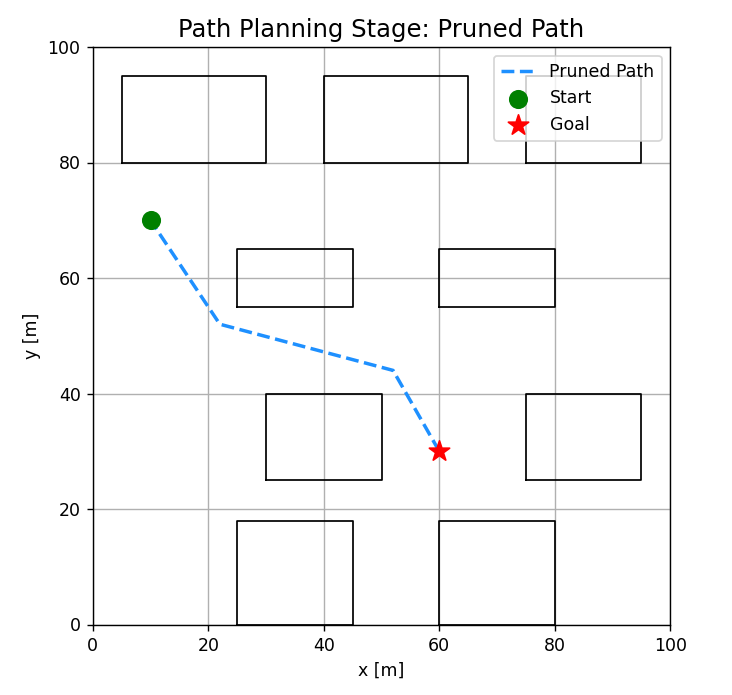
\includegraphics[width=0.7\textwidth]{pruned.png}
	\caption{Pruned path with redundant waypoints removed}
	\label{fig:pruned}
\end{figure}

The results of the pruning process are shown as a blue dashed line. Now the path is shorter and cleaner, due to the removal of redundant waypoints. This condensed path can be processed and followed much easier by the motion controller, which reduces the amount of computing resources required without compromising the obstacle avoidance.


% ─── Step 4 ──────────────────────────────────────────────────────────────────
\subsection{Step 4: Smoothing the Path}

All trimming methods resulted in the same ending, which was still a string of rectilinear segments, rounded at the corners. The last stage was to employ cubic spline interpolation to expertly integrate each of these components into a single continuous line.

The blue curving trajectory depicted in the illustration is the outcome. This arc-like trail is softer for the robot to follow than sharp bends. This is important as it means that a robot moving along a smooth curve can maintain a steady speed and not have to slow down for every turn. The smoothed trajectory is passed onto the following stage.


\begin{figure}[H]
	\centering
	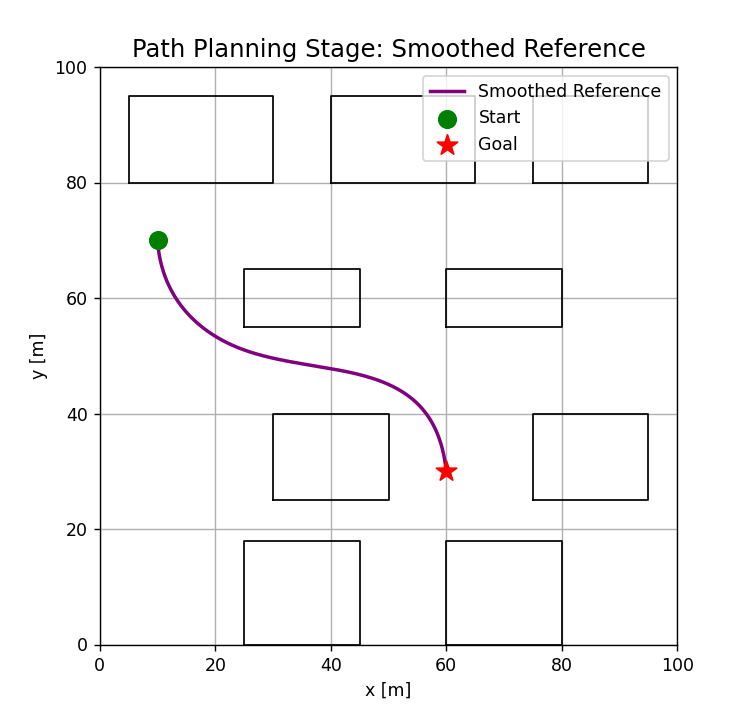
\includegraphics[width=0.7\textwidth]{smooth.png}
	\caption{Final smoothed trajectory using cubic spline interpolation}
	\label{fig:smooth}
\end{figure}

The blue curve is the final curve obtained by doing cubic spline interpolation. The road is now a continuous stream and is curved, with no sharp corners. This enables the robot to move without stopping at any turn, without slowing down during the trip, and will give smoother, more efficient motion.
% ══════════════════════════════════════════════════════════════════════════════
\section{Phase 2: Motion Control with MPC}

A Model Predictive Controller (MPC) was employed to enable the robot to accurately follow the generated reference path.

MPC looks ahead, which is the main distinction between it and a more straightforward controller like PID. It employs a short-term prediction of where the robot will be over the next few steps and modifies its motions accordingly, rather than only responding to where the robot is right now. Because it may begin slowing down or changing direction prior to a turn rather than after it has already missed it, this greatly improves its ability to handle curves.


The MPC was first implemented using a simple model of the robot, which
made it easier to test and tune the controller's core tracking behaviour. Once this
was working well, the MPC was reimplemented using the actual TurtleBot3 kinematic
model, so the controller respected the robot's real velocity limits and motion
constraints. All later tracking tests, including those in Gazebo, use this
TurtleBot3-based version of the MPC.% ─── Basic Test ──────────────────────────────────────────────────────────────
\subsection{Basic Tracking Test}

The blue line indicates the intended reference trajectory whereas the orange line indicates the real path taken by the robot. These two curves are nearly intersecting, which indicates that the controller had high level of precision at the beginning.

The plots on the right hand side illustrate the velocity and acceleration of the robot throughout the period of time in the experiment. The robot has these profiles and no unstable excursions or sharp spikes in the profiles that would indicate that the robot ran in an unexpected manner or impediment was encountered during the run which would have caused these spikes.

\begin{figure}[H]
	\centering
	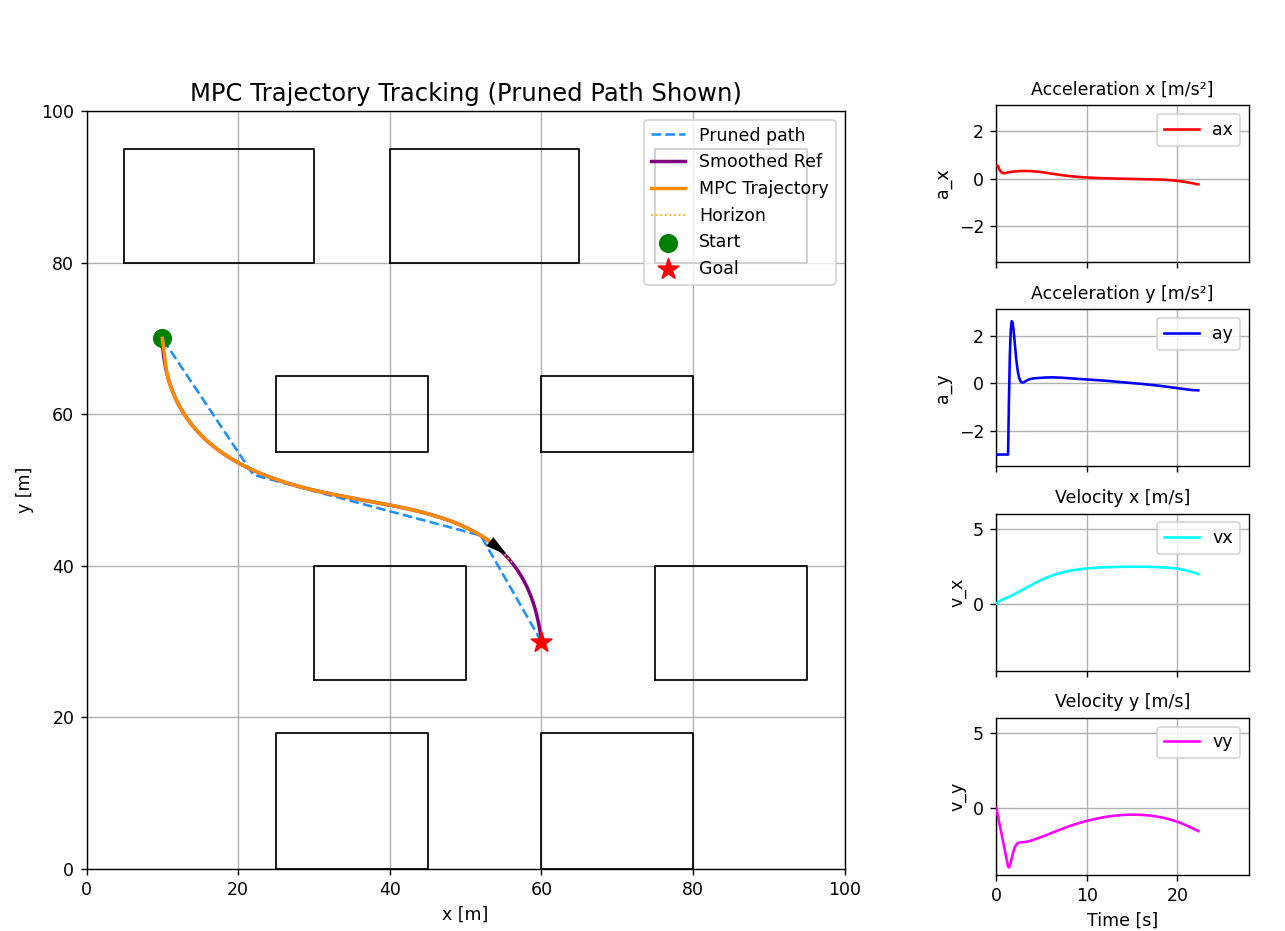
\includegraphics[width=0.85\textwidth]{MPC 1.png}
	\caption{MPC tracking test results}
	\label{fig:mpc1}
\end{figure}

The figure collectively depicts the MPC controller's tracking performance. The orange curve matches the purple curve along the reference path's side plots over the entire time span, with smooth velocity/acceleration plots indicating controlled, inconspicuous motion by the robot without abrupt and erratic transitions.


% ─── Dual Scenario ───────────────────────────────────────────────────────────
\subsection{Testing in Two Different Environments at Once}

The controller was tested in a maze with very small corridors (Scenario~1) and in a large open space (Scenario~2), to ensure that it does not just work very well in one specific map. This comparison against the side was useful in establishing not only the MPC's tuning to a specific configuration, but also as a means of establishing reliability.


\subsubsection{Start of the Mission}

The robot (green dot) is at the start of its path in each map. The orange dotted line extending forward shows the controller's short-term prediction the window of future movement it is planning for at any given moment. Both environments loaded correctly and the MPC was ready to begin tracking.

\begin{figure}[H]
	\centering
	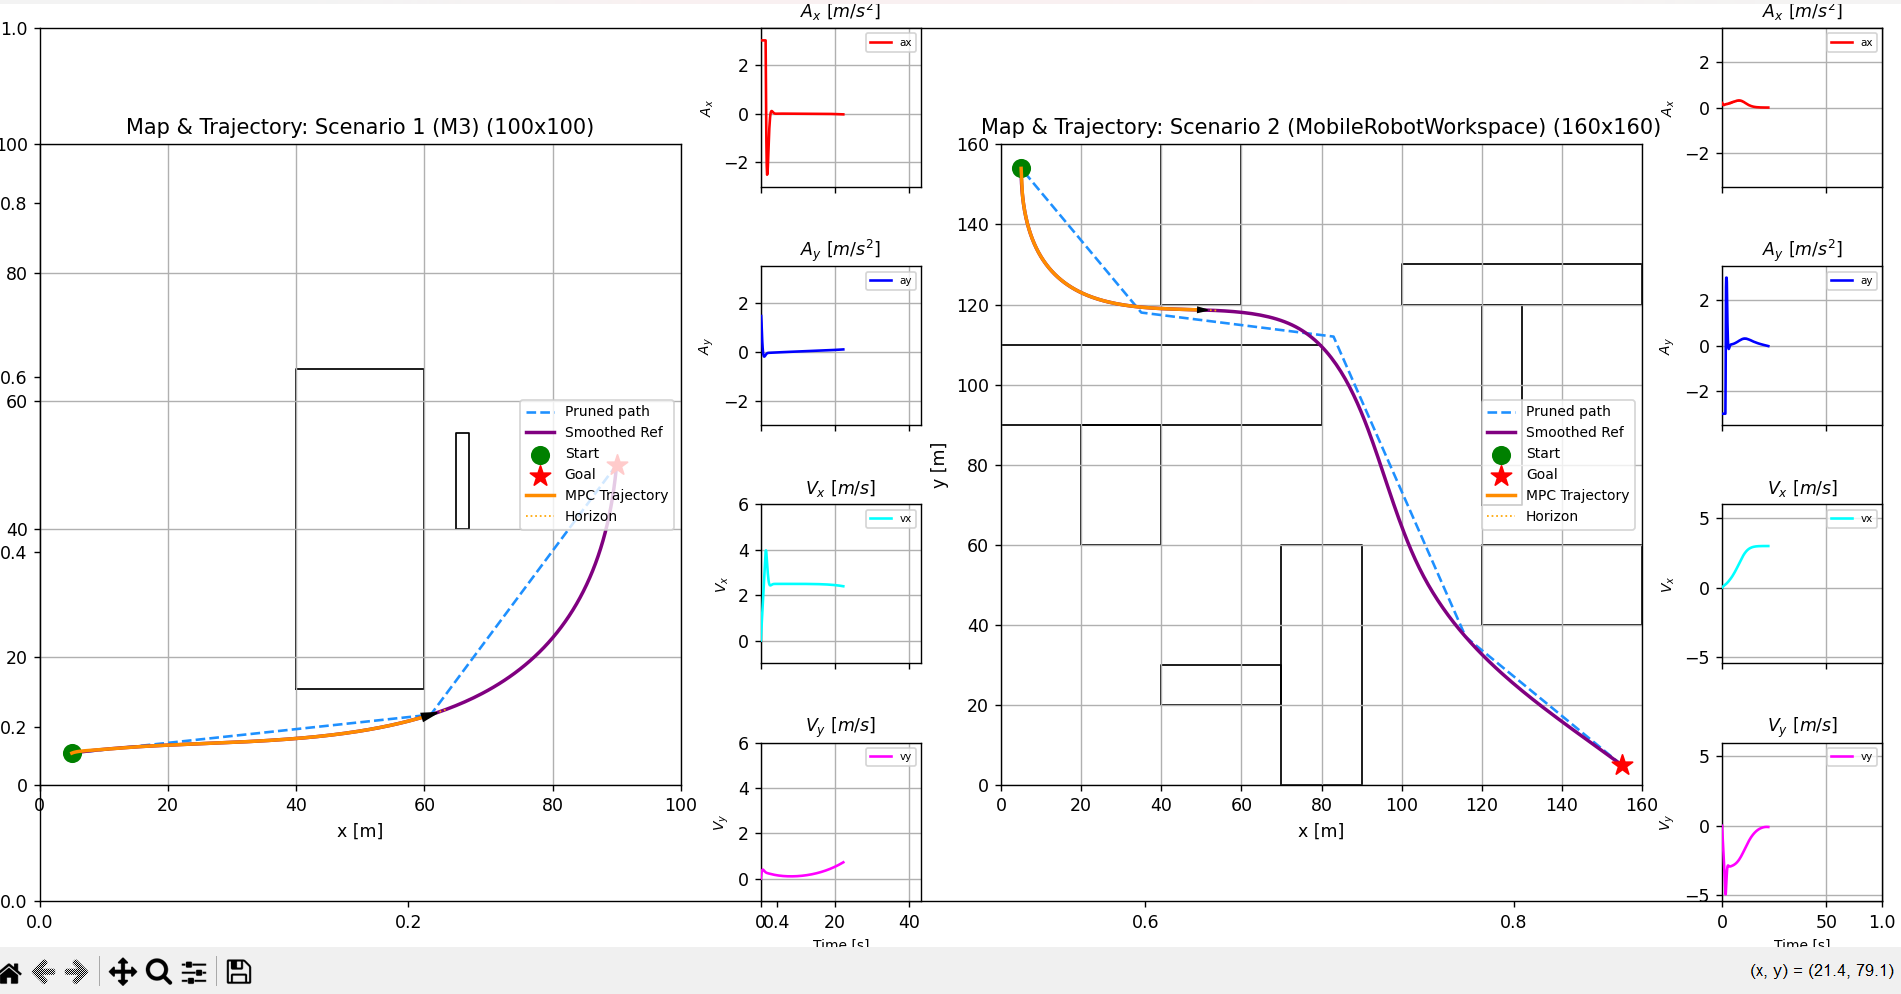
\includegraphics[width=0.9\textwidth]{MPC(start).png}
	\caption{Both environments at mission start}
	\label{fig:mpc_start}
\end{figure}

The figure shows both test environments at the beginning of the mission. The green dot represents the robot's starting position in each scenario. The orange dotted line extending forward illustrates the MPC's lookahead prediction horizon, showing the short-term future movement window that the controller is actively planning for at this instant.

\subsubsection{End of the Mission}

Once both runs completed, the orange path the robot actually took falls almost perfectly on top of the planned purple path in both maps. Whether navigating tight corners in the maze or covering a large open distance, the controller maintained the same level of accuracy throughout confirming the system is not sensitive to map layout.

\begin{figure}[H]
	\centering
	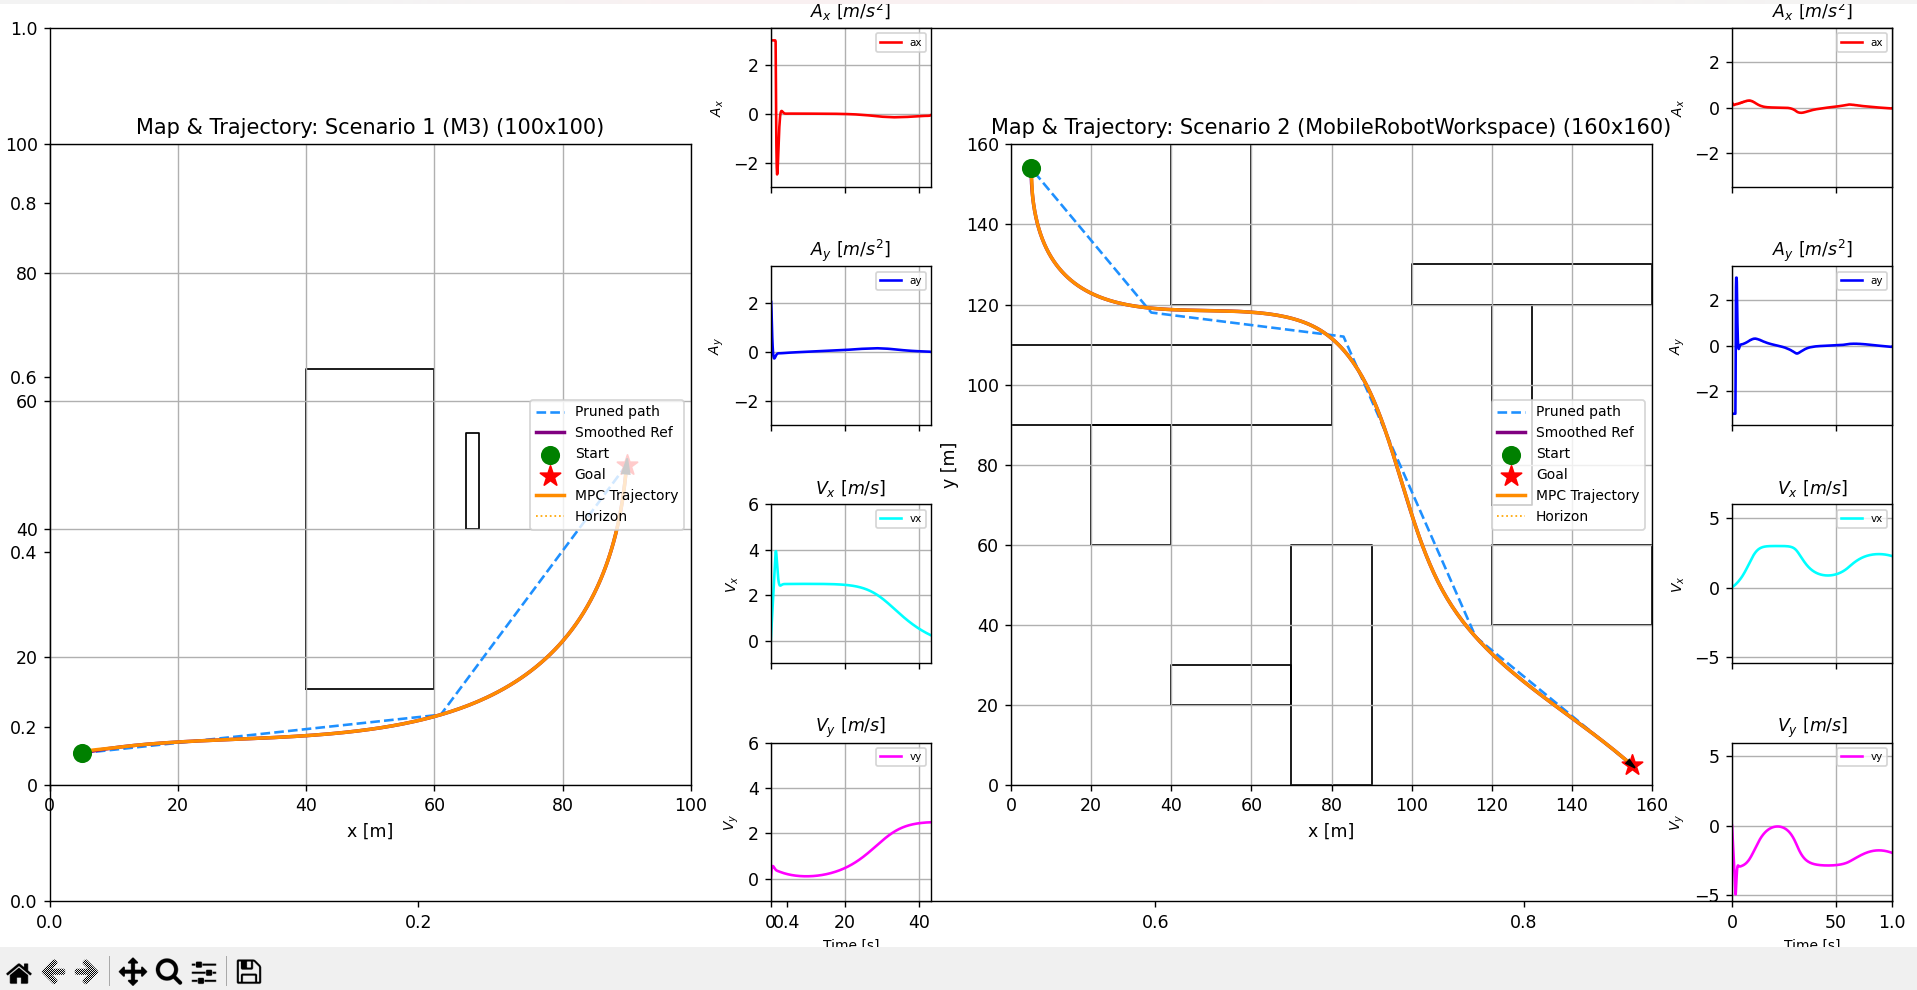
\includegraphics[width=0.9\textwidth]{MPC(end).png}
	\caption{Both environments at goal convergence}
	\label{fig:mpc_end}
\end{figure}

The successful completion of mission is shown in both environments, as seen in the image \ref{fig:mpc_end}. The orange real path is shown on top of the purple reference path in both cases, with consistent tracking accuracy in both cases, regardless of the complexity of the surroundings. The MPC controller does a good job in different map layouts and situations of navigation.


% ─── Error Analysis ──────────────────────────────────────────────────────────
\subsection{Measuring the Tracking Error}
While it can be useful to simply look at the paths, it is more useful to determine the actual error of the controller. In both cases, the deviation of the robot from the reference path (cross-track error) was observed at any time.


\subsubsection{Scenario 1: Standard Maze}

There is a slight increase in inaccuracy at the beginning of the run. The robot is accelerating from a standstill and briefly exceeding the speed before slowing down—typical. The inaccuracy decreases to almost zero after a few seconds. There are brief, little bumps throughout the maze's rapid curves, but they go away fast. The error was still significant when moving at constant speed (2~cm).


\begin{figure}[H]
	\centering
	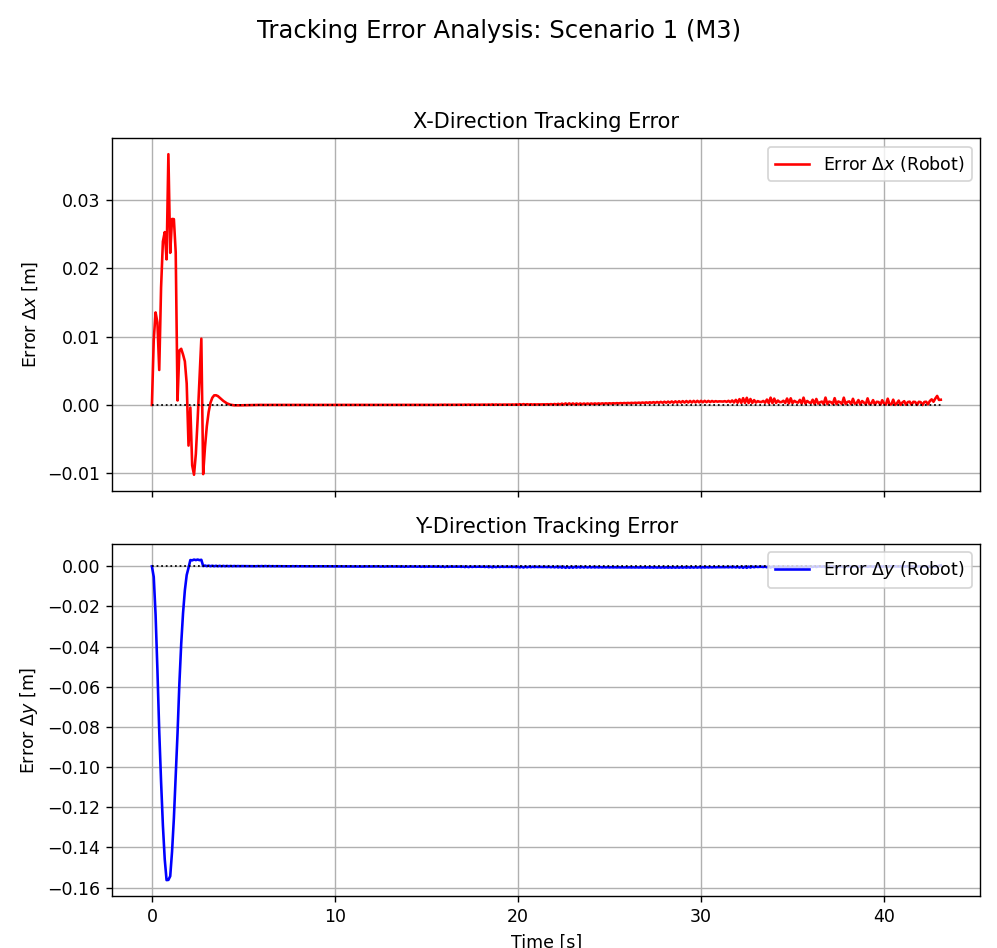
\includegraphics[width=0.85\textwidth]{Tracking Error Analysis S1.png}
	\caption{Tracking error analysis for Scenario 1}
	\label{fig:error_s1}
\end{figure}

The cross track error for the maze environment with time is shown in the figure. Inaccuracy quickly settles into almost a constant value after an initial transient upon startup and remains below 2~cm throughout the trip. Its ability to navigate tight corners with little error can be seen in the quick correction of the errors that occur at the corners.The controller's ability in difficult to navigate situations, with tight bends, is shown by the brief error spikes that occur at steep curves followed by quick corrections.


\subsubsection{Scenario 2: Large Open Workspace}

Compared to the maze, the open workspace yielded an even smoother error profile. The error signal was not fluctuating much during the bulk of the run and the amount of corrective action performed by the controller was less since there were fewer sharp corners to overcome. This shows the MPC to be capable and effective in less demanding situations and competent in more demanding situations.


\begin{figure}[H]
	\centering
	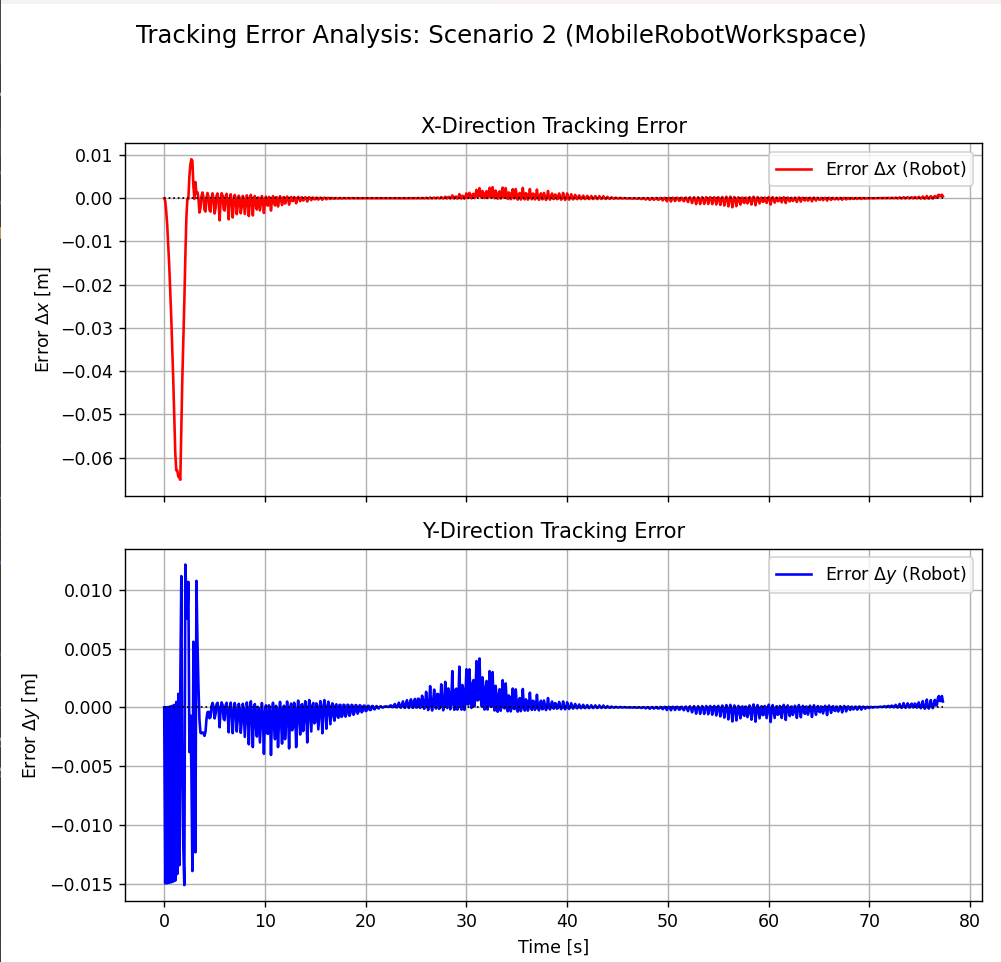
\includegraphics[width=0.85\textwidth]{Tracking Error Analysis S2.png}
	\caption{Tracking error analysis for Scenario 2}
	\label{fig:error_s2}
\end{figure}

The error profile in the open workspace will be quite flat as there are fewer requirements for curvature. The controller works better in regions with relatively few limits as it keeps the tracking error extremely small during the entire course of the mission in less challenging spaces with lesser sharp bends. 



% ─── Stress Test ─────────────────────────────────────────────────────────────
\subsection{Stress Test: Circles and Triangles}

To this end, a specially designed map with irregularly shaped obstacles in the form of triangles and circles has been constructed, in order to further test the motion controller. This led to very restricted and cumbersome routes. Because these non-orthogonal designs produce sharp angles and curved sides that call for quick and precise navigational maneuvers, they are more challenging to handle than the more conventional rectangular barriers.   

The little openings the robot navigated through weren't blocked and the bot didn't get confused.
Its path sensorimotor remained in a steady flow even as it manoeuvred around the sharp corners of triangular shapes hence proving that the Model Predictive Control scheme has the ability to cope with the challenging geometries just as easily as simpler ones.
\begin{figure}[H]
	\centering
	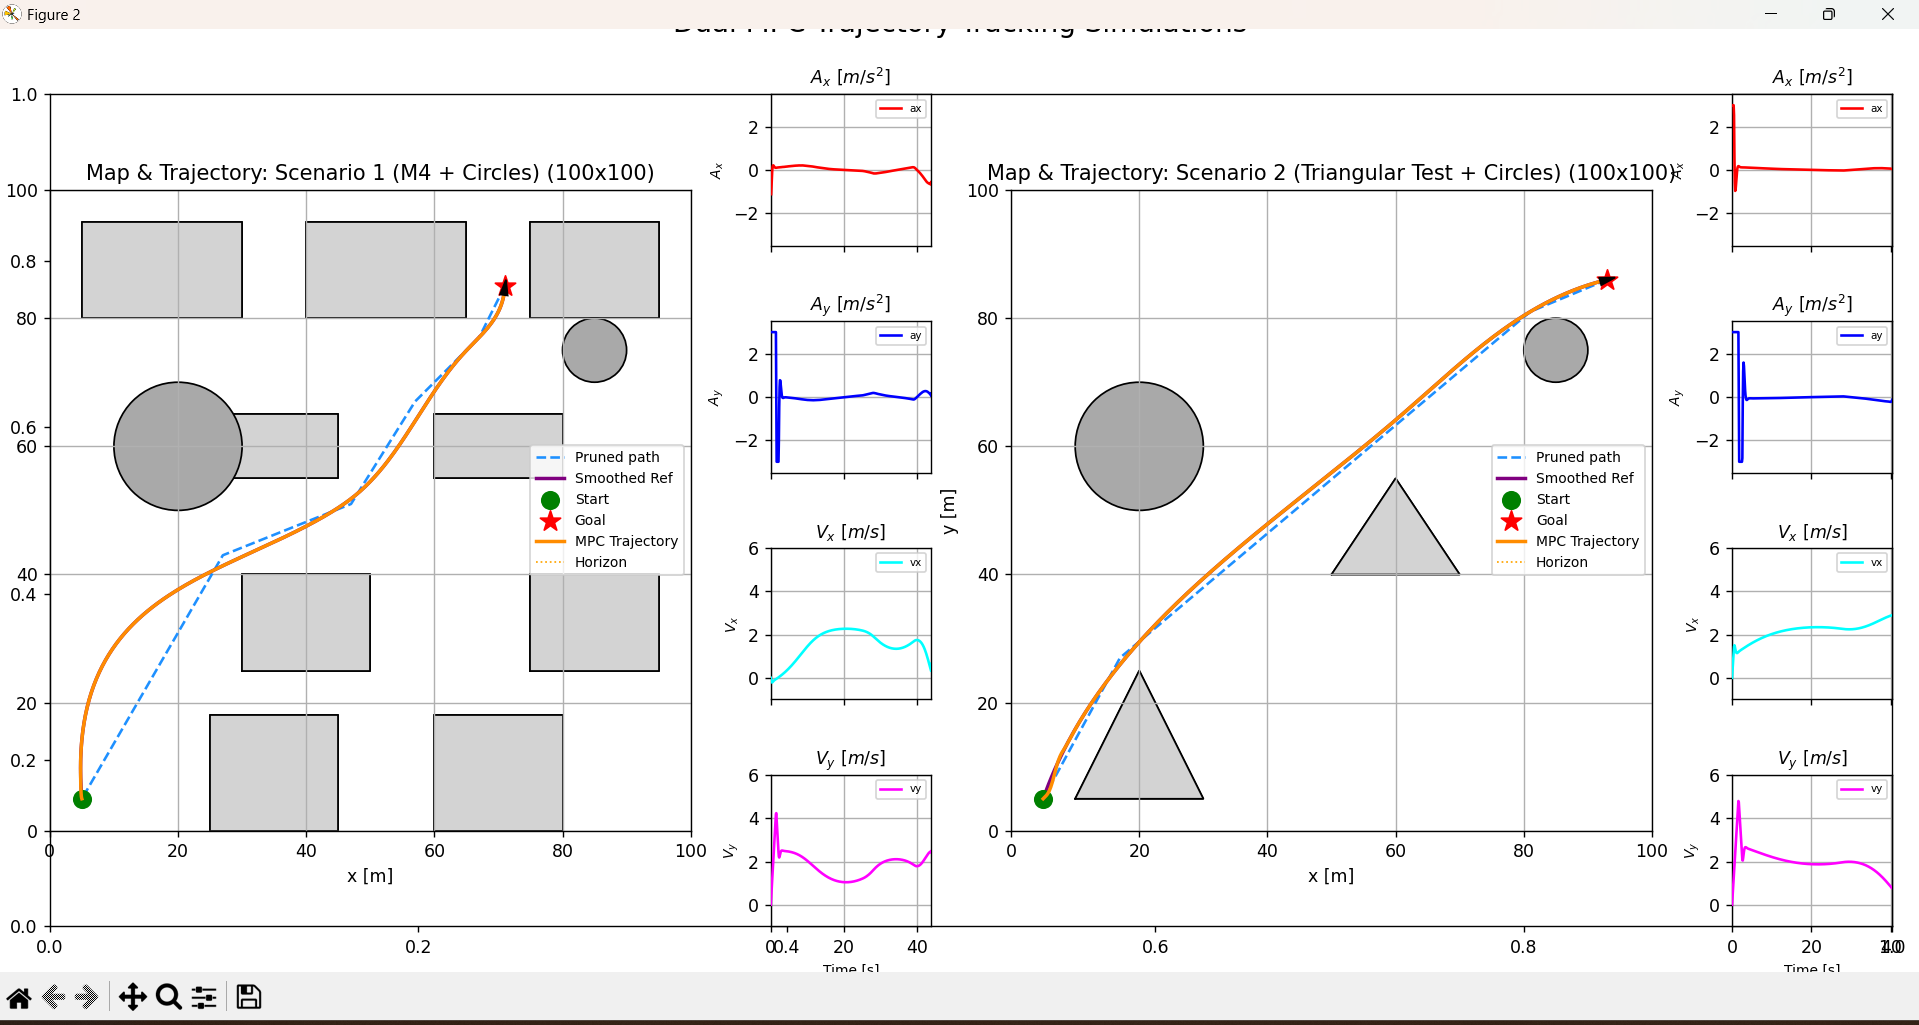
\includegraphics[width=0.85\textwidth]{MPC(Circle+triangle).png}
	\caption{Stress test with circular and triangular obstacles}
	\label{fig:mpc_complex}
\end{figure}

The controller's performance with complicated obstacle geometries is shown in figure \ref{fig:mpc_complex}. The robot maintains a smooth course while successfully navigating every narrow space between triangular and circular obstacles. This confirms that the MPC can manage complex geometric arrangements and unusual obstacle shapes that call for quick, accurate trajectory modifications.


\subsection{TurtleBot3 Model Tracking of PSO-Smoothed Path}

Dedicated tracking simulations were performed on both test maps using the TurtleBot3's motion parameters in order to confirm that the MPC controller could consistently track the PSO-smoothed path while adhering to the kinematic and velocity constraints of the real TurtleBot3 robot model. Each graphic displays the MPC trajectory superimposed on the same map as the trimmed A* path, the PSO control points, and the resulting PSO-smoothed path.


\subsubsection{Start of the Tracking Run}

Both possibilities are displayed at the start of the tracking run in Figure~\ref{fig:pso_mpc_start}.
The trimmed A* path (blue dashed line) in each map has previously been optimized into a smooth continuous trajectory (green line) and transformed into a set of PSO control points (orange squares). In both the compact map and the larger MobileRobotWorkspace map, the MPC trajectory (solid orange line) produced by the TurtleBot3 kinematic model is just starting to follow this smoothed reference from the start position (green dot) toward the goal (red star). As the controller begins tracking while staying within the TurtleBot3's operational parameters, the side plots display the initial acceleration and velocity response.


\begin{figure}[H]
	\centering
	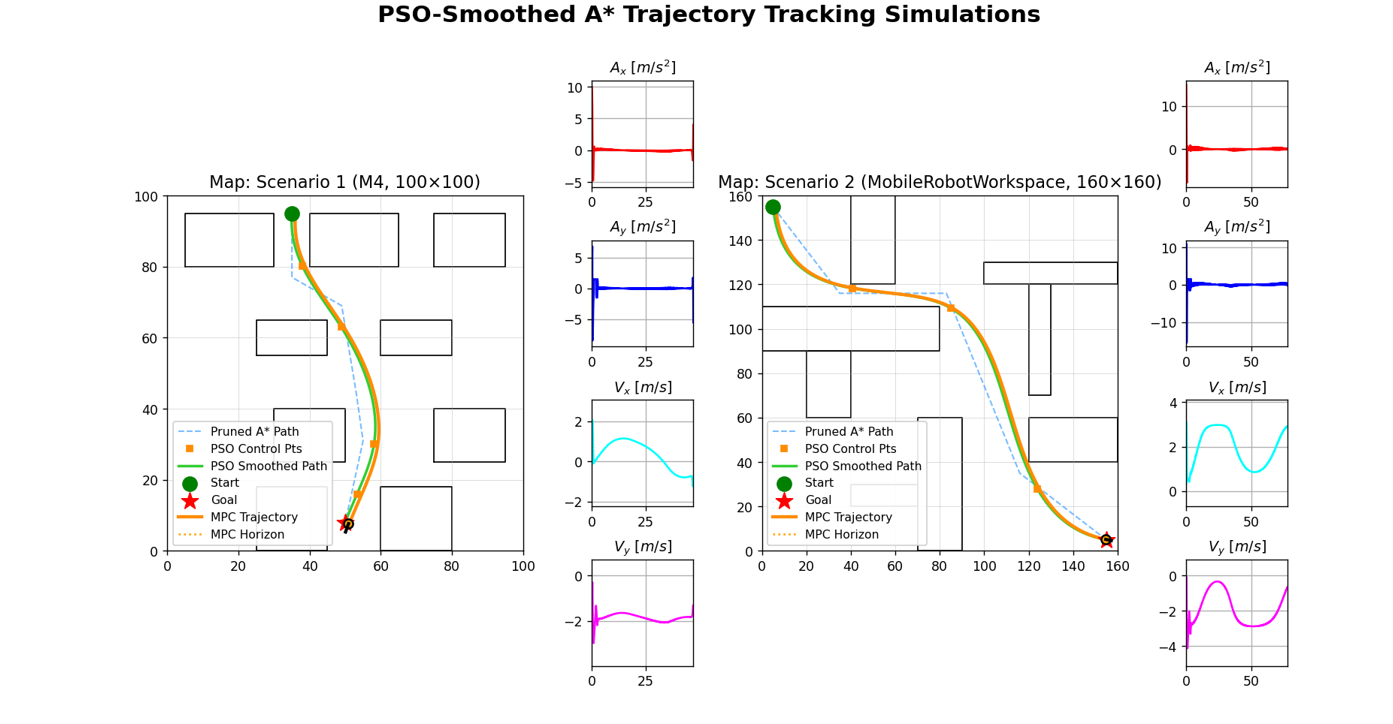
\includegraphics[width=1\textwidth]{pso_mpc_tracking_start.png}
	\caption{TurtleBot3 Model MPC Tracking of the PSO-Smoothed A* Trajectory at the Start of the Mission}
	\label{fig:pso_mpc_start}
\end{figure}

\subsubsection{End of the Tracking Run}

Both scenarios are displayed at the end of the tracking run in Figure~\ref{fig:pso_mpc_end}.
Now that the MPC trajectory has successfully reached the goal location in each scenario, it nearly perfectly covers the whole length of the PSO-smoothed path in both maps. The controller maintained steady, low-jerk motion compatible with the TurtleBot3's kinematic limitations from beginning to end, as seen by the acceleration and velocity profiles remaining smooth throughout.


\begin{figure}[H]
	\centering
	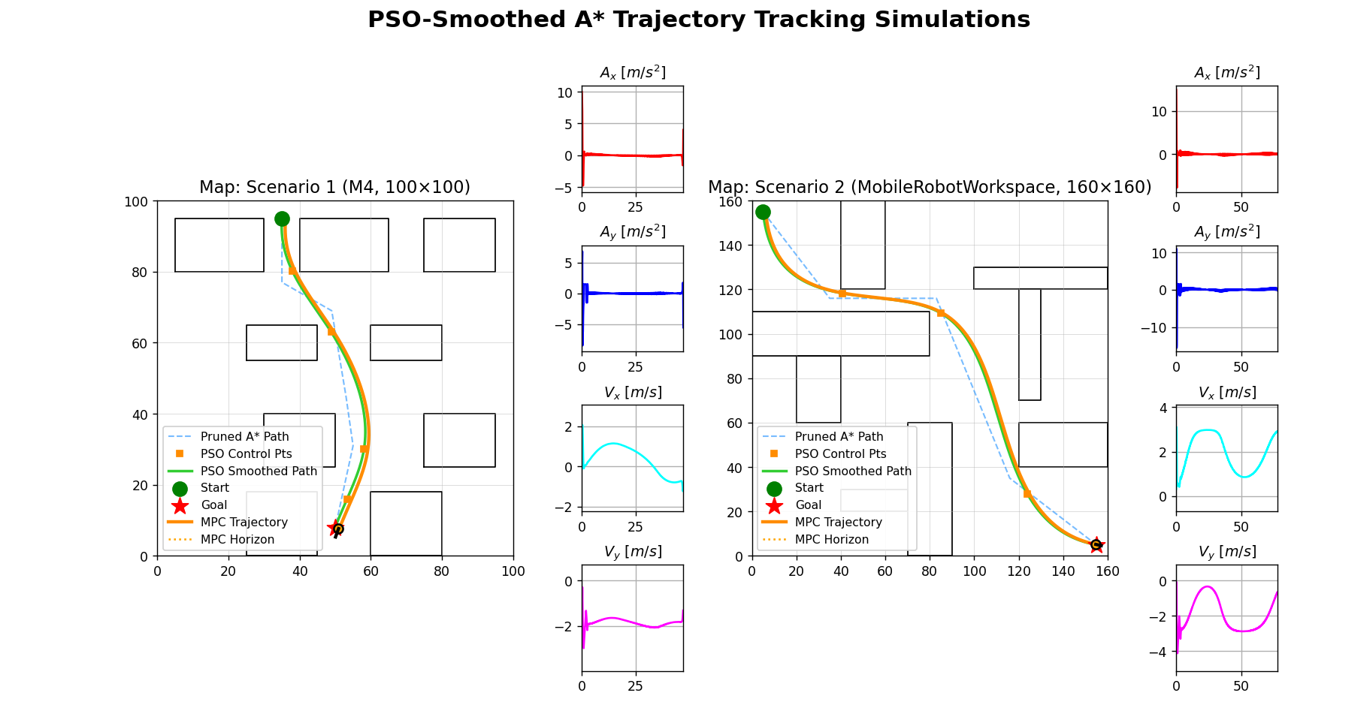
\includegraphics[width=1\textwidth]{pso_mpc_tracking_end.png}
	\caption{TurtleBot3 Model MPC Tracking of the PSO-Smoothed A* Trajectory at the End of the Mission}
	\label{fig:pso_mpc_end}
\end{figure}

These findings verify that, regardless of map size or obstacle layout, the MPC controller, set up with the TurtleBot3's kinematic model, precisely tracks the PSO-smoothed reference path from start to goal, generating smooth, low-jerk motion profiles consistent with the robot's real-world motion capabilities.


\subsection{Keeping the Robot Safe: Obstacle Inflation}
One crucial safety feature that is integrated into the navigation backend is obstacle inflation. The algorithm is used not on the physical obstacle itself, but on a mathematical expansion of the footprint of the obstacle, which forms a virtual "no-go" buffer zone.


Figure \ref{fig:inflation} visualizes this mechanism clearly. The diagram differentiates between two distinct zones:
\begin{itemize}
	\item \textbf{Original Obstacle:} 
	The core area is light pink and is used to indicate what the object physically would look like.
	
	\item \textbf{Inflated Obstacle:} 
	The outer drawing is the safety buffer as drawn by the algorithm and is drawn in deeper red.
\end{itemize}

Hard limit is the Inflated edge, the path planner is forced to keep distance to the physical object (the robot). This essentially supplies the uncertainties encountered in the real world, such as sensor noise, or small localization errors, and thus the robot (initially in the green marker) will never hit the wall when working towards the goal (red square).



\begin{figure}[H]
	\centering
	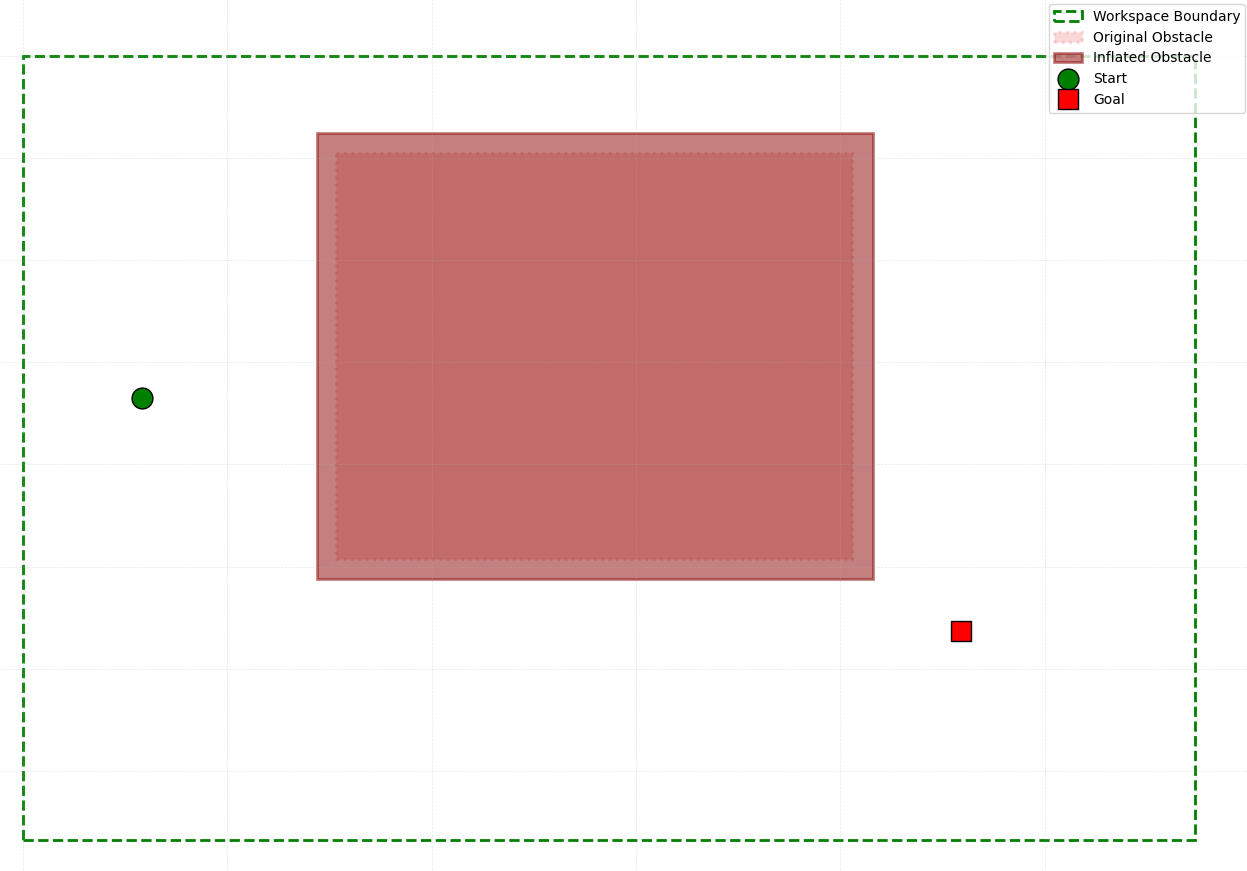
\includegraphics[width=0.8\textwidth]{inflation.png} 
	\caption{Obstacle inflation}
	\label{fig:inflation}
\end{figure}

% ══════════════════════════════════════════════════════════════════════════════
\section{Phase 3: Web Interface}

When the basic algorithms were successful, a web-based control interface was created to enable a person to observe the robot and set the delivery tasks without any code or ROS~2. Making the system usable by everyone, not just technical experts, was the aim.


% ─── Dashboard ───────────────────────────────────────────────────────────────
\subsection{The Control Dashboard}

A particular interface for mission planning is the control dashboard. The system will ultimately be able to accept custom facility maps or Point Cloud Data (PCD), but for the purposes of this demonstration it is based on an OpenStreetMap layer to provide a realistic visual context.

The interface follows a structured, step-by-step workflow to ensure secure path generation:
\begin{enumerate}
	\item \textbf{Define Workspace:} To define the robot's safe working area, the operator first chooses the "Draw Boundary" option.

	\item \textbf{Place Obstacles:} Next, users can draw virtual obstacles (using Rectangle or Circle tools) to represent restricted zones, such as construction areas or temporary hazards.
	\item \textbf{Assign Mission:} Finally, the operator marks the exact Start point (Green Marker) and End point (Red Marker) which characterize the delivery task.
	
\end{enumerate}
When this configuration is accomplished, the static map information is fed into the backend computational routines and the optimal trajectory is calculated. This configuration based architecture will enable non-technical staff to gain the ability to conduct safe and effective designation of the environment the robot will operate in, before implementation.
\begin{figure}[H]
	\centering
	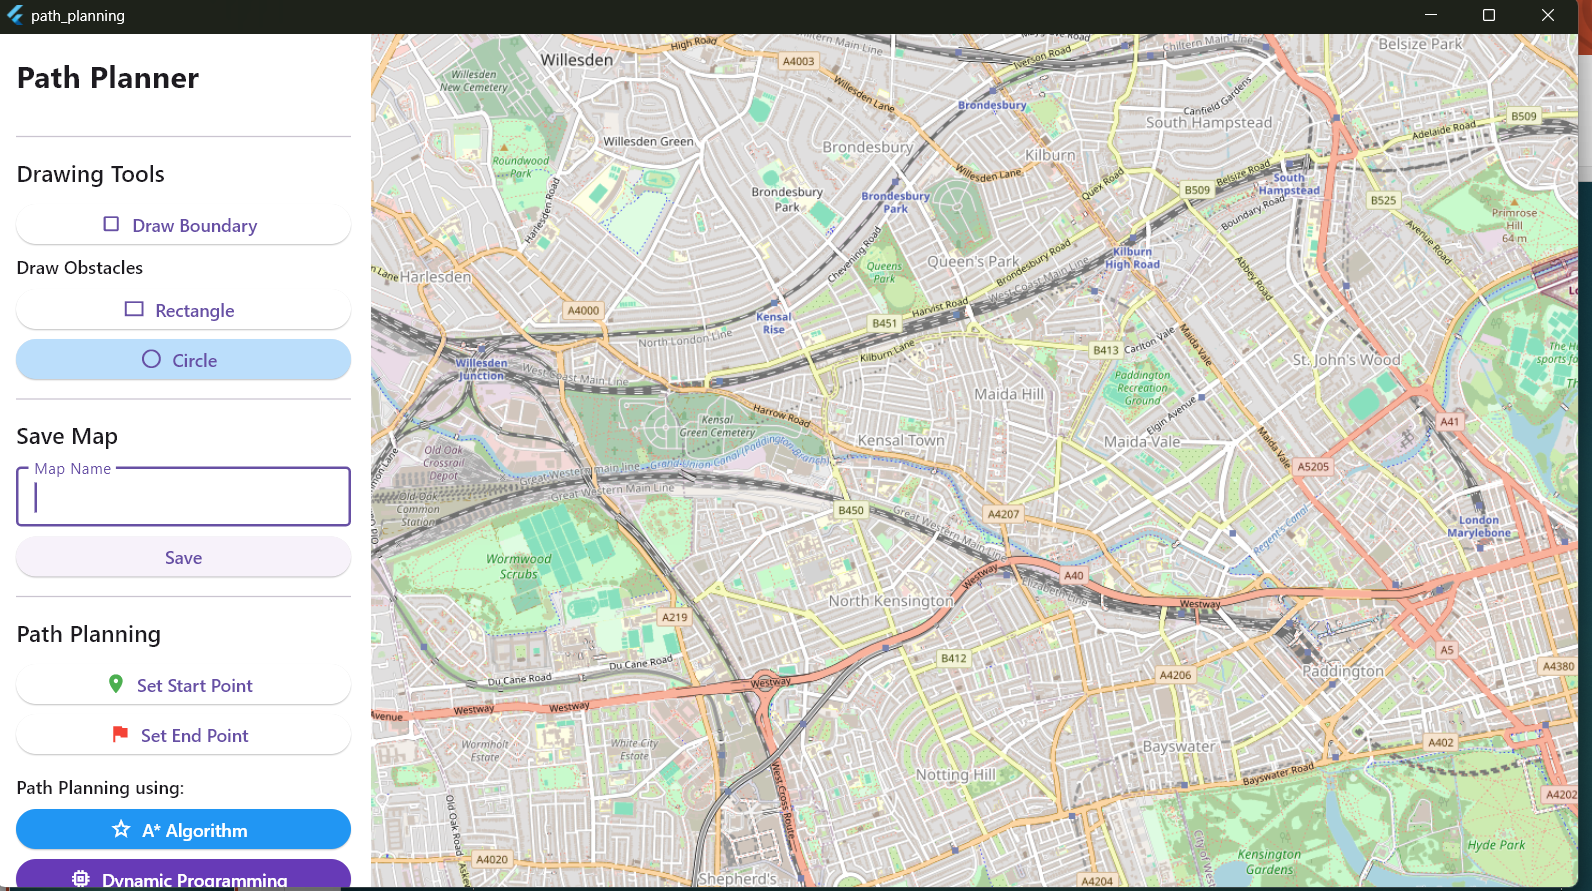
\includegraphics[width=0.95\textwidth]{webapp.png}
	\caption{Web control dashboard used for defining boundaries, obstacles, and mission points}
	\label{fig:webapp}
\end{figure}
% ─── Inflation ───────────────────────────────────────────────────────────────
\section{2D Global Planner Results}

We ran the global planner on the 2D map environment first before entering the full 3D simulation. The aim of those tests was ensuring that the planner is capable of producing safe and correct paths in varying obstacle layouts. A 2D version allows us to exercise sanity of the path planning code without wasting time on robot dynamics, sensor noise or real-time control issues.

In order to assess the planner correctly we established three scenarios. Each scenario was tailored to test a unique factor, one that entailed obstacle avoidance with an adequate safety margin, one to avoid blocking obstacles, and the final was to plan distances on a larger scale on a cluttered map.
\subsection{Cellular Decomposition Output (2D Workspace Partitioning)}
In order to make global navigation in a complex indoor setting simple, we adopted a cellular decomposition method on the 2D workspace. The primary aim of this step is to divides into several non-overlapping areas (cells) the free space according to the boundaries of obstacles. The cells are safe zones where the robot will not run into anything.

Once the cells are decomposed, A representative point (cell center) is chosen for each region. These centers are then used to build an adjacency graph of connectivity.This graph helps the planner to easily determine a possible route from start to finish, and provides a simplified, high level structure of the environment.


Figure~\ref{fig:cellular_decomposition} shows the final output of the cellular decomposition
process, including the generated cells, their connectivity, and the resulting global path.
The planned route demonstrates how the robot transitions between cells while avoiding
obstacles and restricted regions.

\begin{figure}[H]
	\centering
	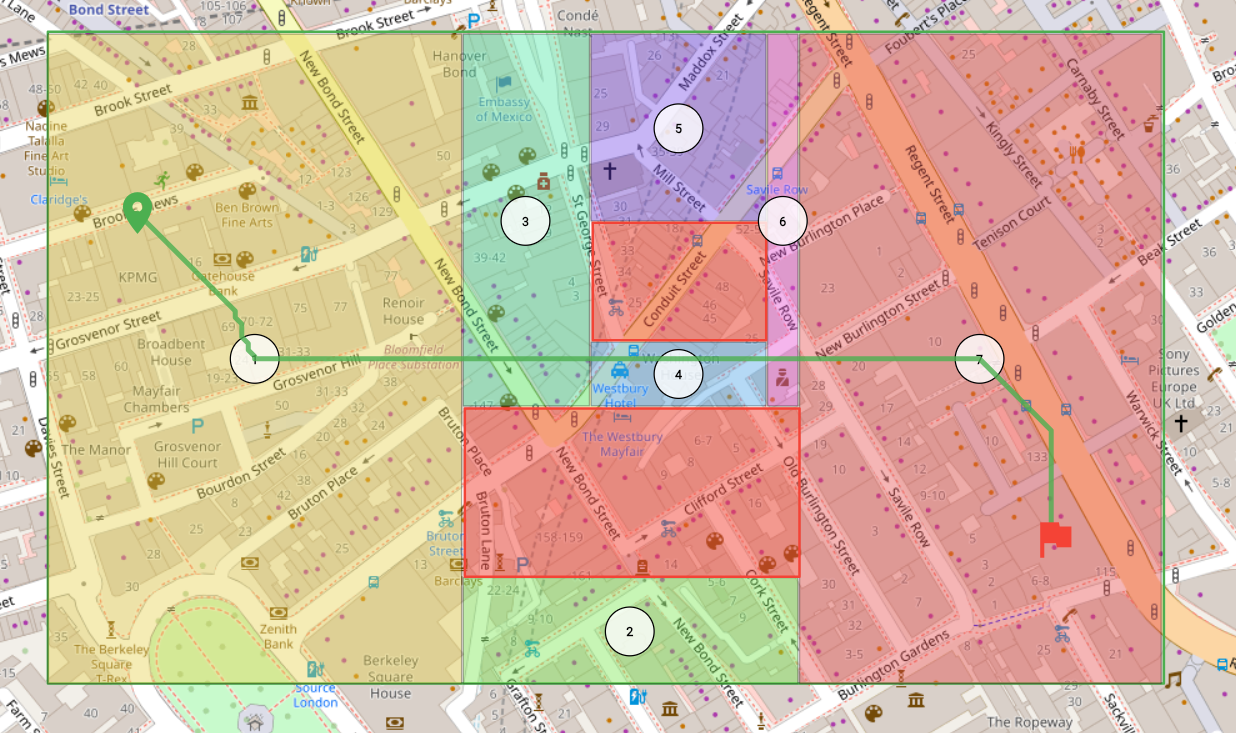
\includegraphics[width=0.8\textwidth]{grid.png}
	\caption{Output of cellular decomposition showing workspace partitioning into cells,
		adjacency connectivity, and the generated global path from start to goal.}
	\label{fig:cellular_decomposition}
\end{figure}


\subsection{Scenario A: Path Planning with Obstacle Avoidance}

In the first test (Figure \ref{fig:scen1}), the planner was given a task to navigate from the start point to the goal while avoiding a large circular restricted zone.The main factor when planning the robotic paths would be the definition of the workspace boundary, which defines the allowed area of operation. The robot has the responsibility of seeing that he does not cross this line, and at the same time, keeps to a predetermined safe distance of any possible dangers.

The importance of the given test is that it allows assessing the skills of the planner in coping with obstacle inflation. The test environment has a circular obstacle surrounding which has been superimposed a safety buffer, a light pink annulus in which is placed a darker core. The planner must be able to make certain that the trajectory of the robot does not trespass on this inflated area, but only avoids the physical limit of the obstacle.

Experimental findings suggest that the planner found a smooth curvy path and was able to maneuver through the obstacle and maintain the necessary clearance distances. Notably, the route does not violate the workspace limitations and infringe upon the limited area, which proves the effectiveness of the adopted safety margin system.

\begin{figure}[H]
	\centering
	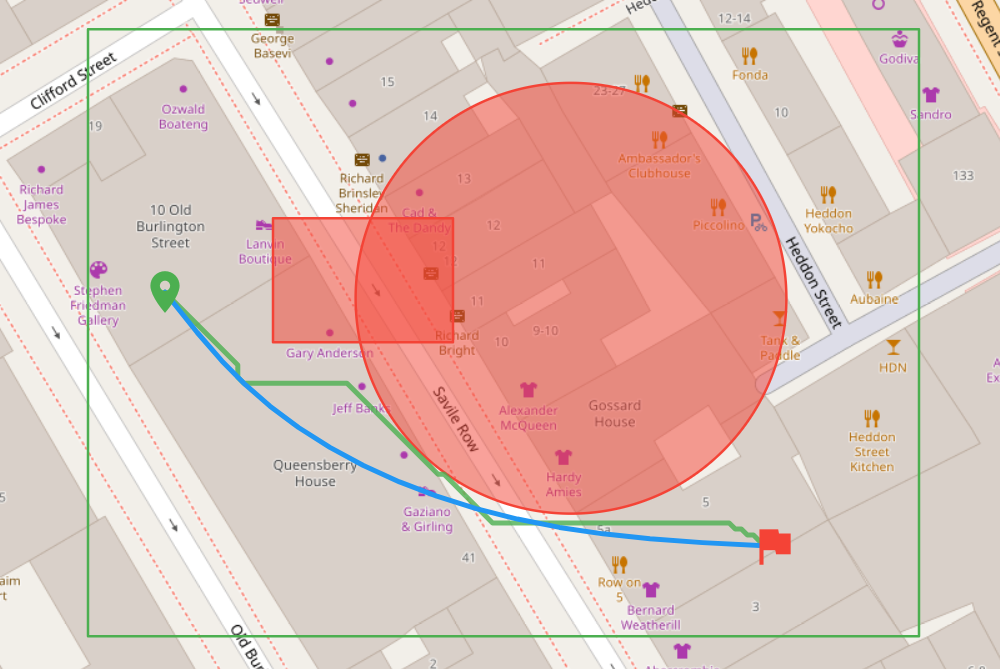
\includegraphics[width=0.7\textwidth]{test2.png}
	\caption{Scenario A: Path planning with obstacle avoidance}
	\label{fig:scen1}
\end{figure}
The findings reveal that the planner was able to find a smooth and curved path that bypasses the obstacle maintaining sufficient clearance. The path also does not go too far in the spatial boundaries of the working area and does not go too close to the limited area. This makes the efficacy of the safety margin system confirmed by these observations.

\subsection{Scenario B: Navigating Around Multiple Obstacles}

The second test (Figure \ref{fig:scen2}) included both a large circular obstacle and a rectangular restricted zone.
The rounded barrier was placed in such a manner that it was on the most direct path of the initial and final destinations forcing the planner to come up with an alternative path.

This scenario will analyse the ability of the planner to solve the cases where straight line path is not possible. In the operational delivery situations, furniture, equipment, or provisional barriers often hinder the shortest path; therefore the robot has to be intelligent enough to avoid these obstacles.

The outcomes prove that the planner generated a smooth detour by which the circular obstacle was circumscribed and the rectangular zone was avoided at the same time. The path experiences a natural curvature towards the obstruction and manages to hit the goal without any accidents.

These results can be attributed to the flexibility of the planner, who restructured the ways in the wake of hindering impediments.

\begin{figure}[H]
	\centering
	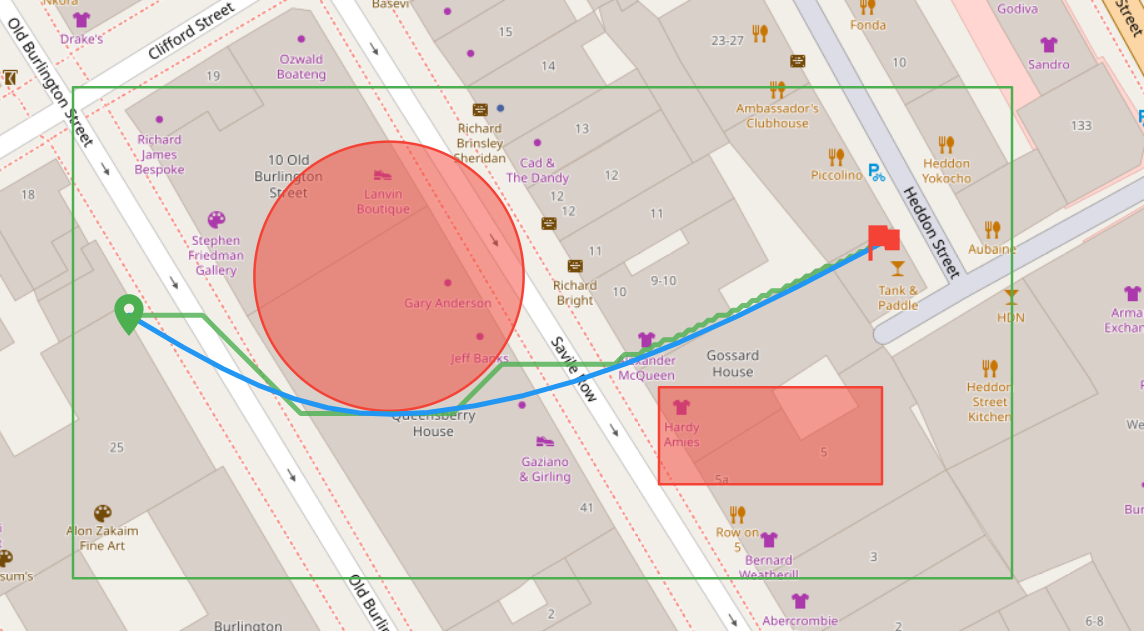
\includegraphics[width=0.7\textwidth]{test3.png}
	\caption{Scenario B: Navigating Around Multiple Obstacles}
	\label{fig:scen2}
\end{figure}

\subsection{Scenario C: Non-Convex Obstacle Negotiation}

The final test (Figure \ref{fig:scen3}) was designed to represent a more realistic delivery scenario.The area of workspace has been extended and a heterogeneous array of obstacles which has different geometry and dimension has been intentionally inoculated into the domain. The robotic platform therefore needs to move through a geodesic that is more significant in distance between its starting point and final goal, but at the same time having to manoeuvre through the ever growing cluttered environment.

This construct is used as a testbed, which is purposive, thus allowing an assessment of the soundness of the planner with respect to dimensional scalability and obstacle density. As the environmental topology continues to add more complexities, some planning methodologies can have a latency increment or worse still, fail to produce a viable answer.

The results of the empirical study confirm that the global planning module has managed to outline a continuous path between the source and the destination. The resulting trajectory sinuously navigates the landscape of forbidden areas, and always maintains the recommended buffer areas in relation to all the barriers it passes. The planner has therefore exhibited strength in increased complexity, and has been able to complete the mission within a reasonable time frame.
\begin{figure}[H]
	\centering
	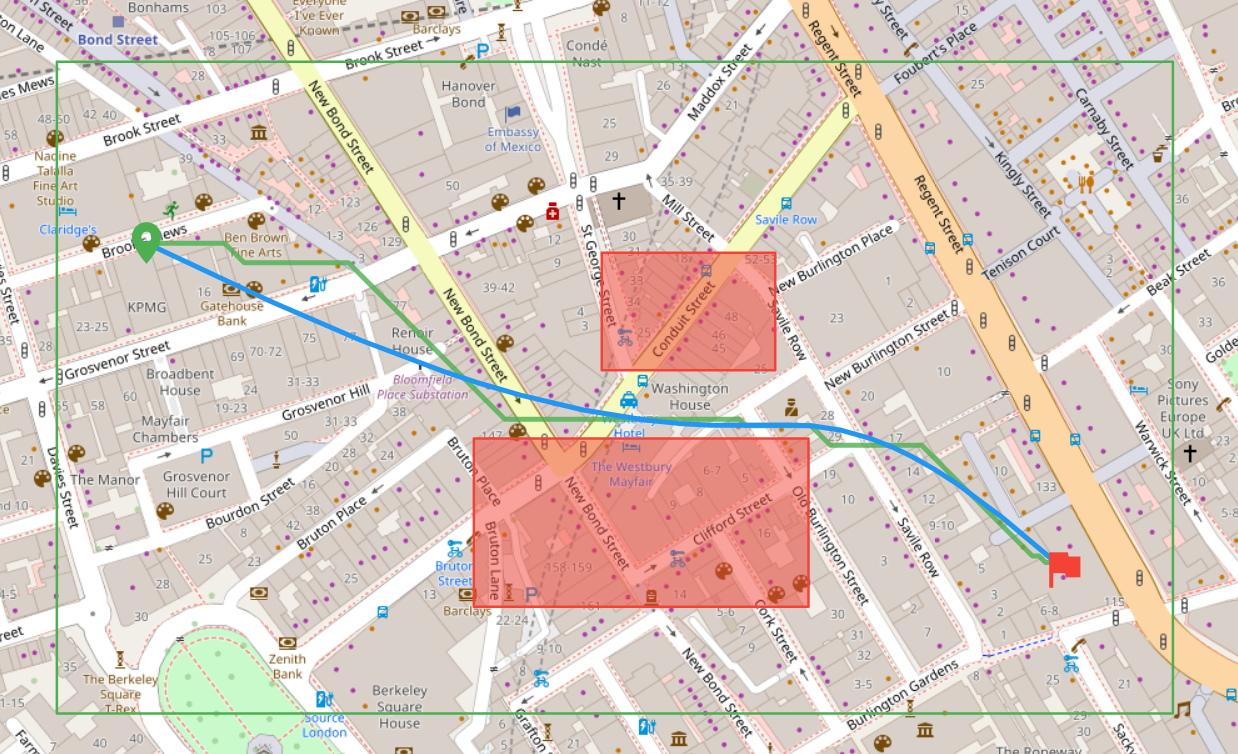
\includegraphics[width=0.7\textwidth]{test4.png}
	\caption{Scenario C: Long-range global planning across a multi-obstacle environment.}
	\label{fig:scen3}
\end{figure}

\subsection{Overall Observation}
In all of these three tests the planner is seen to be working extremely well in a range of two dimensional situations. It skillfully avoids obstacles with keeping the safety margins required, finds effective paths in case the current one is blocked, and moves on to larger and more complicated maps without any degradation.

Results act as confidence measures for the proper functioning of the path-planning algorithm even prior to the addition of the complexity of three-dimensional simulation. The planner will be tested in the ROS 2 and Gazebo settings in the next phase dynamic obstacles will be introduced.

\section{Phase 4: Flutter Web Application for Delivery Management}

While the dashboard described in Section 5.3 was used early in the project to validate map-based path planning, the delivery task itself is issued and monitored in practice through a dedicated Flutter web application built for end users, dispatch staff, and system administrators. The following section show the various screens of that application, including user authentication, requests for delivery, floor plan selection (with interaction), and administration tools for editing the facility map.

\subsection{Starting screen and Authentication}

The web starts with a simple presentation page showing a brief description of the system and its purpose before leading the user to the authentication interface.


\begin{figure}[H]
	\centering
	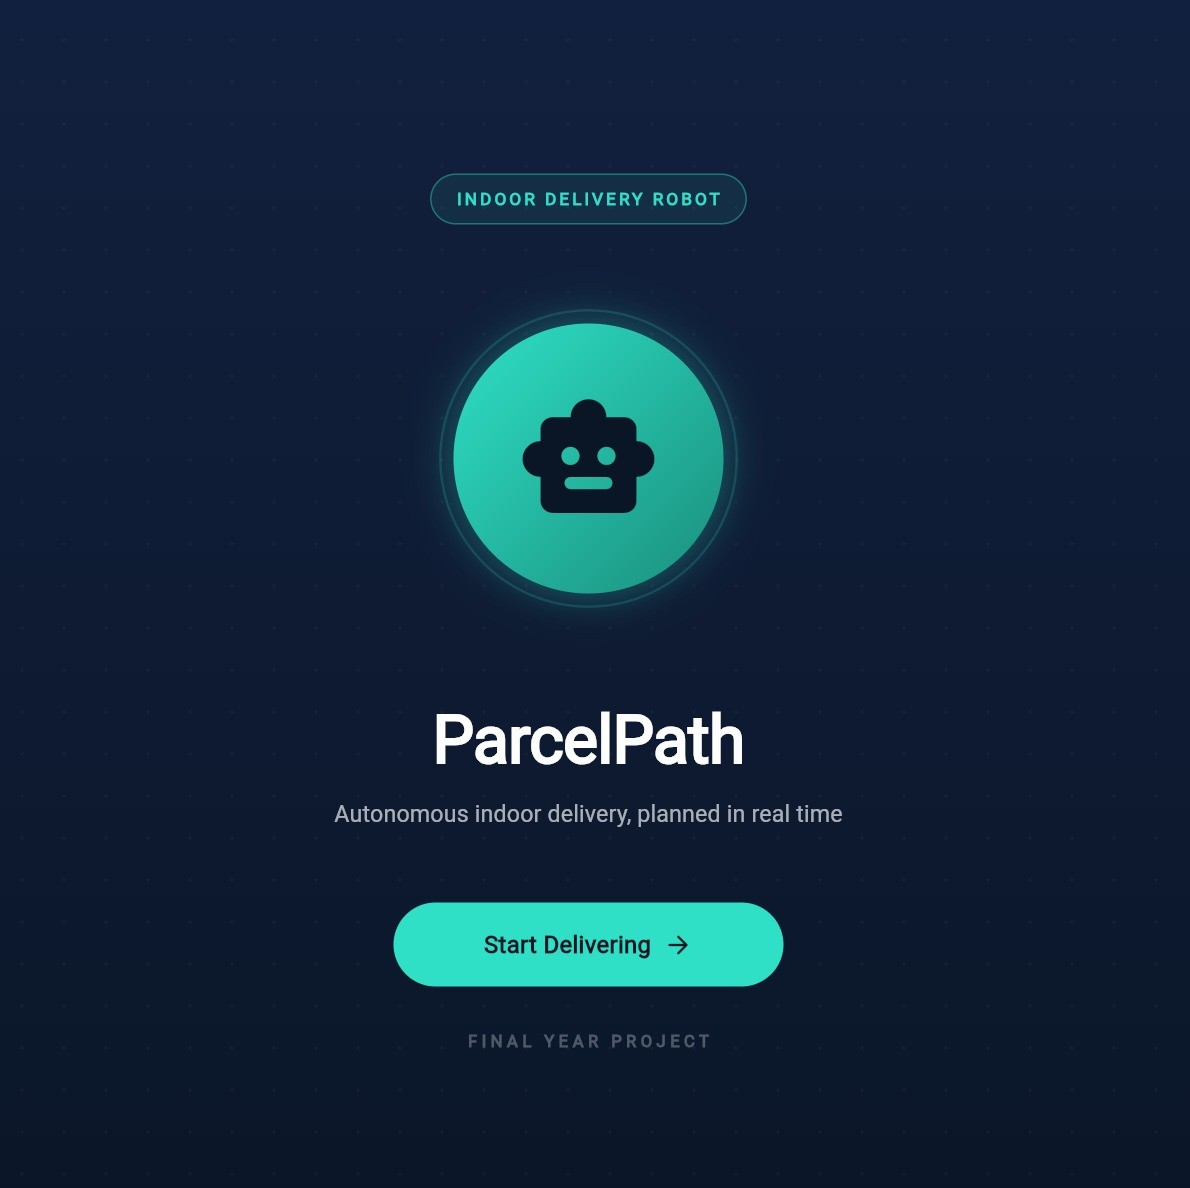
\includegraphics[width=0.5\textwidth]{starting_screen.jpeg}
	\caption{starting screen of the ParcelPath web application}
	\label{fig:starting_screen}
\end{figure}

The starting screen (figure~\ref{fig:starting_screen}) welcomes the user to the system in the name of “Indoor Delivery Robot” and presents the name ParcelPath with the tagline: “Autonomous indoor delivery, planned in real time”. The "Start Delivering" button takes the user forward in the authentication process.

On returning users, the system redirects them to the login screen as shown in Figure~\ref{fig:login} and requires them to log in with their registered email and password to gain access to the delivery portal, while in case of a new user, he is redirected to sign up page as shown in Figure~\ref{fig:signup} where he enters his details such as full name, registered email and password to sign up.


\begin{figure}[H]
	\centering
	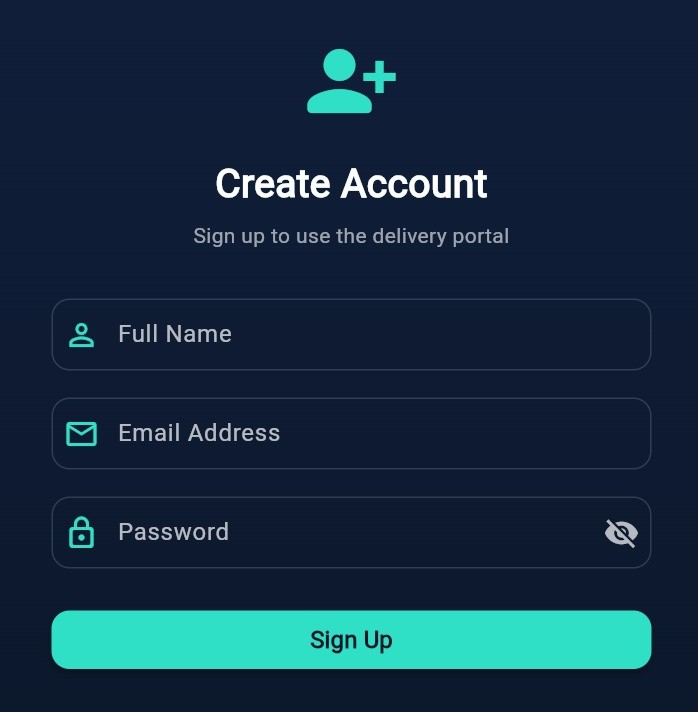
\includegraphics[width=0.5\textwidth]{Sign_up_page.jpeg}
	\caption{Account registration screen for new users}
	\label{fig:signup}
\end{figure}

\begin{figure}[H]
	\centering
	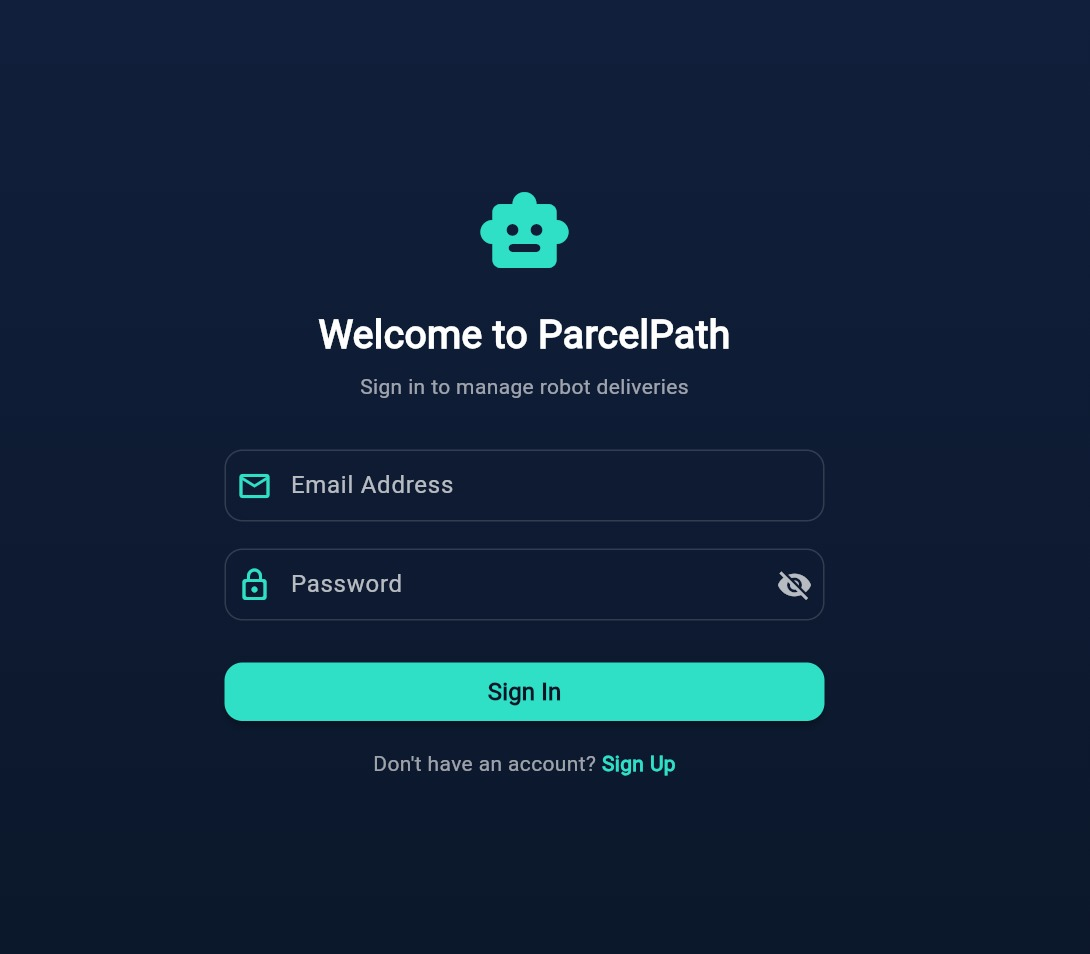
\includegraphics[width=0.5\textwidth]{Login_page.jpeg}
	\caption{Login screen used to authenticate returning users}
	\label{fig:login}
\end{figure}

Both forms have masked password fields with a visibility toggle, and a link to the sign up form for users who haven't already signed up.

\subsection{User Portal and Delivery Requests}

Once authenticated, the user is taken to the User Portal, shown in Figure~\ref{fig:user_portal}, which serves as the main hub for requesting and monitoring deliveries.

\begin{figure}[H]
	\centering
	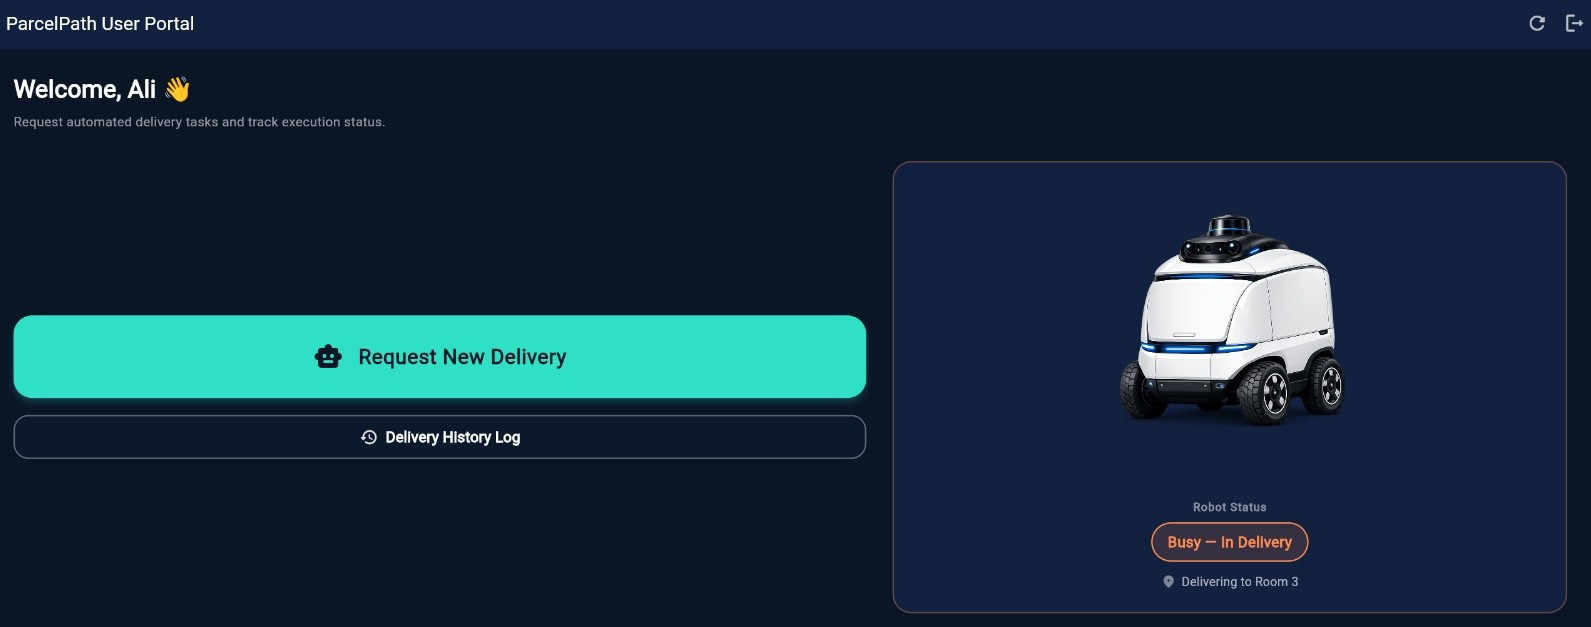
\includegraphics[width=0.9\textwidth]{user_interface.jpeg}
	\caption{User portal showing delivery request options and live robot status}
	\label{fig:user_portal}
\end{figure}

"Request New Delivery," which opens the delivery request form, and "Delivery History Log," which displays previously accomplished deliveries, are the two main activities that the portal offers to the logged-in user after greeting them by name. The robot and its current state—in this case, "Busy - In Delivery"—as well as its current destination are rendered on the status card on the right, providing the user with real-time visibility into robot activity without requiring them to explicitly examine ROS subjects.


Selecting "Request New Delivery" opens the interactive delivery request form shown in Figure~\ref{fig:dispatch_form}.

\begin{figure}[H]
	\centering
	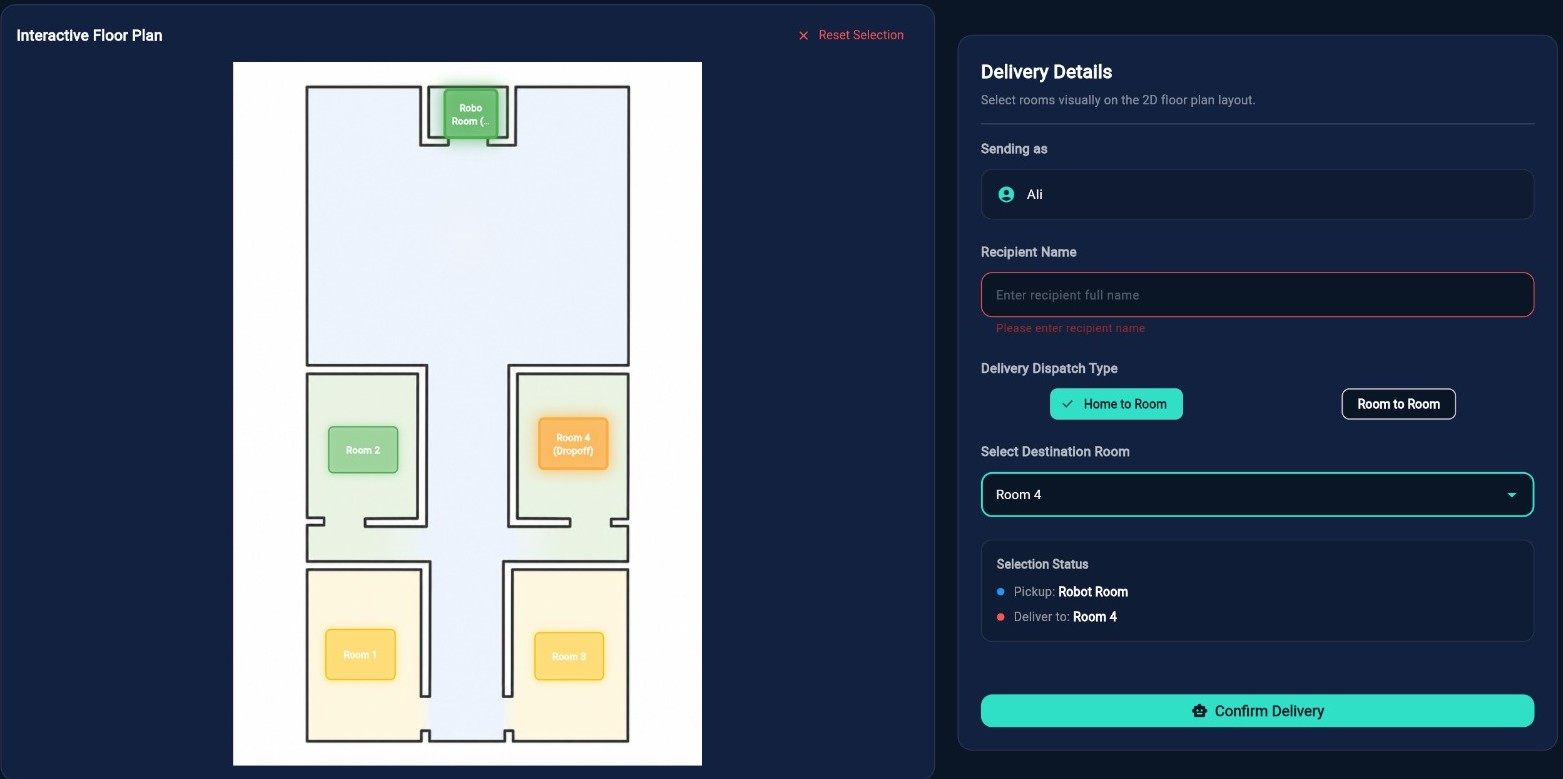
\includegraphics[width=0.95\textwidth]{Dispatching_detail_form.jpeg}
	\caption{Delivery request form with interactive floor-plan room selection}
	\label{fig:dispatch_form}
\end{figure}

Each room is depicted as a selectable colored block in the left panel, which shows the same floor plan used to create the Gazebo world (Figure~\ref{fig:2dmap}). Before the request can be made, the recipient's name must be entered in the Delivery Details panel on the right, which automatically fills in the sender's name from the logged-in account. "Home to Room" or "Room to Room" are the two dispatch kinds that the user can select. The destination can be tapped directly on a room in the floor plan or selected from a dropdown menu. Before the user completes the request with the "Confirm Delivery" button, which transforms the chosen rooms into the matching ROS navigation coordinates and sends the task to the robot, a live "Selection Status" summary verifies the resolved pickup and drop-off rooms.


\subsection{Administrator Operations Hub}

System administrators are directed to a separate Admin Operations Hub, shown in Figure~\ref{fig:admin_hub}, rather than the delivery request screen used by regular users.

\begin{figure}[H]
	\centering
	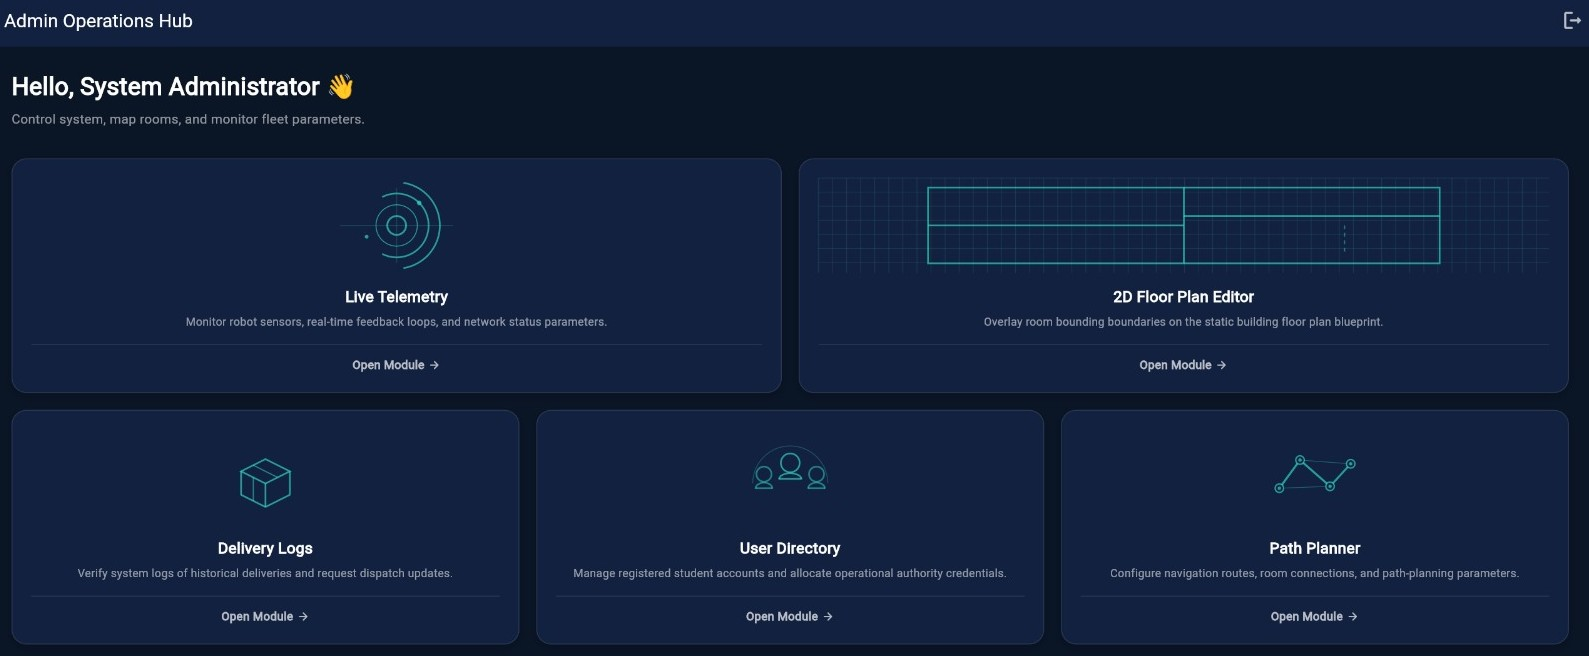
\includegraphics[width=0.95\textwidth]{admin_interface.jpeg}
	\caption{Admin Operations Hub providing access to fleet monitoring and configuration modules}
	\label{fig:admin_hub}
\end{figure}

The hub divides administrative tasks into five modules: the Path Planner, which configures navigation routes, room connections, and planning parameters; the User Directory, which manages registered accounts and access levels; the 2D Floor Plan Editor, which overlays room boundaries on the facility blueprint; Delivery Logs, which examines the historical record of completed and pending deliveries; and Live Telemetry, which monitors robot sensors, feedback loops, and network status in real time. With its own "Open Module" link, each module can be opened separately.


\subsection{2D Floor Plan Editor}

The 2D Floor Plan Editor, opened from the Admin Operations Hub, allows the administrator to map each physical room to its corresponding coordinates in the robot's navigation frame, so that room selections made in the user-facing delivery form (Figure~\ref{fig:dispatch_form}) resolve to valid goal poses for the robot.

\begin{figure}[H]
	\centering
	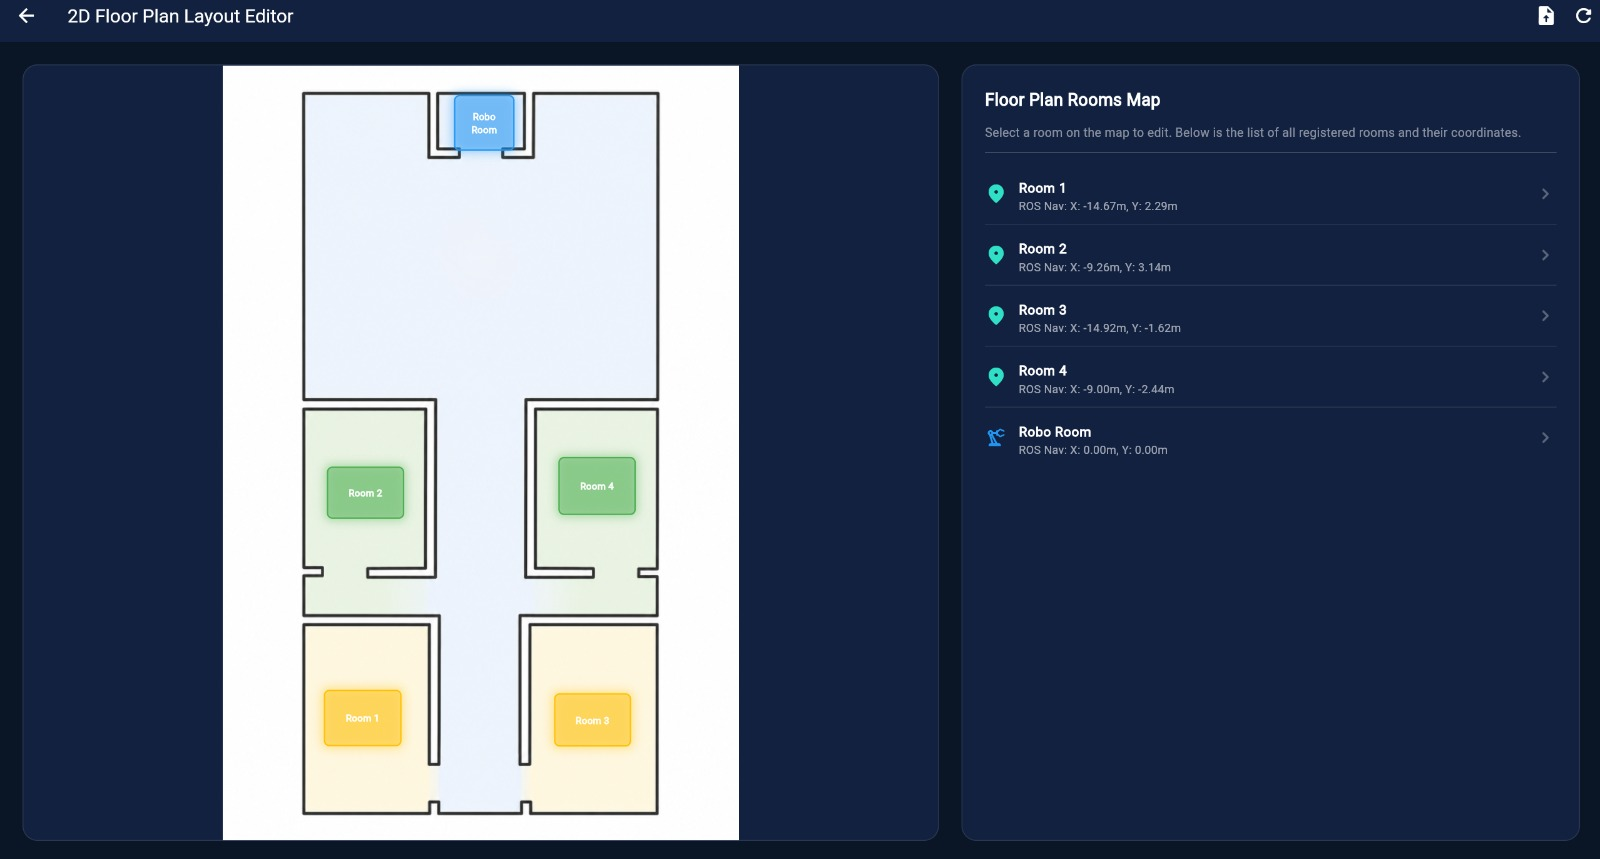
\includegraphics[width=0.95\textwidth]{2d_plan_editor_opt_from_admin_interface.jpeg}
	\caption{2D Floor Plan Layout Editor listing all registered rooms with their ROS navigation coordinates}
	\label{fig:plan_editor_list}
\end{figure}

Figure~\ref{fig:plan_editor_list} shows the floor plan on the left, with each room drawn as a coloured block, alongside a "Floor Plan Rooms Map" list on the right enumerating every registered room, including the robot's own home position ("Robo Room"), together with its stored ROS navigation X and Y coordinates in metres. Selecting a room from this list, or tapping it directly on the map, opens the corresponding editing controls.

\begin{figure}[H]
	\centering
	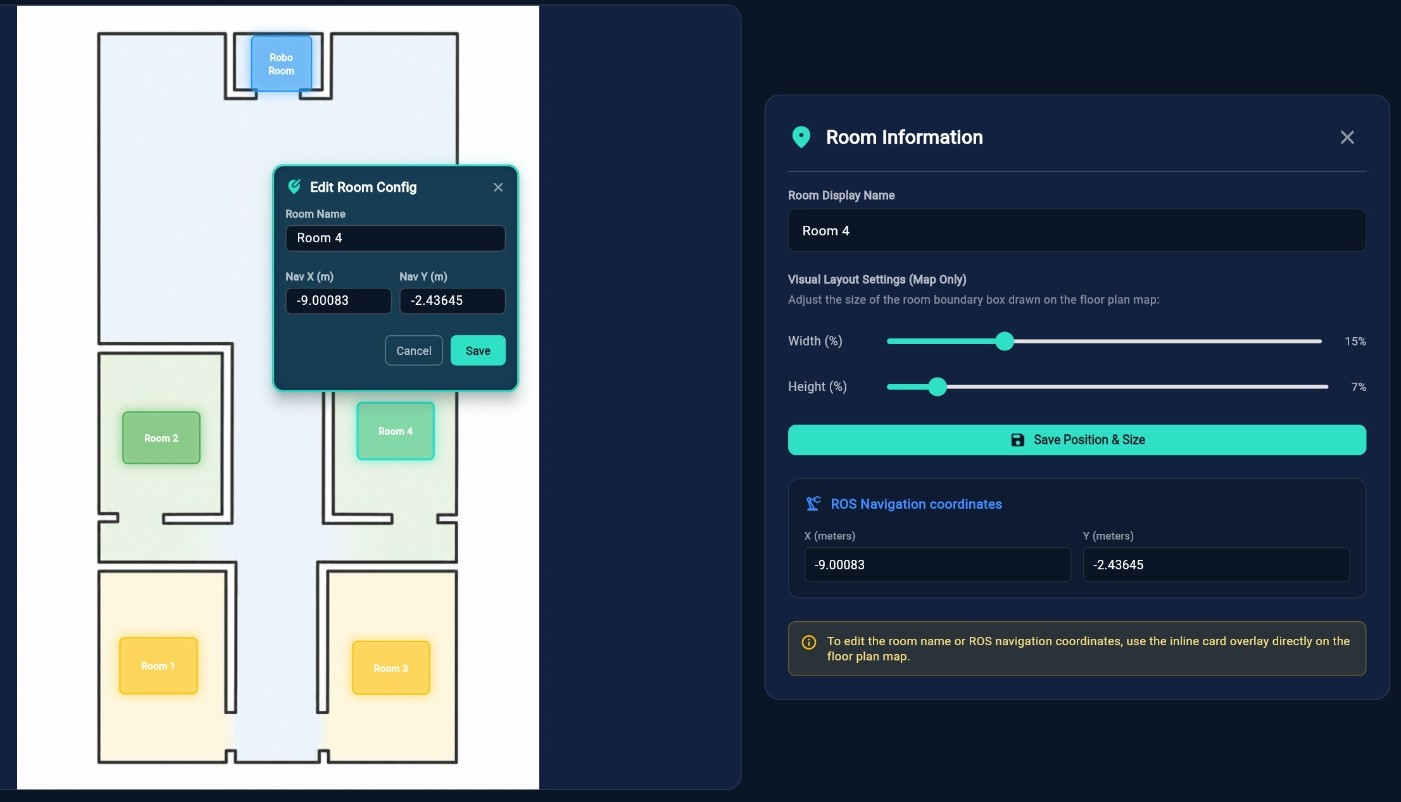
\includegraphics[width=0.95\textwidth]{2d_plan_editor_options_for_changing_sch_as_coordinates.jpeg}
	\caption{Room configuration panel for editing a room's display name, ROS navigation coordinates, and on-map bounding box}
	\label{fig:plan_editor_edit}
\end{figure}

As shown in Figure~\ref{fig:plan_editor_edit}, selecting a room opens an "Edit Room Config" dialog together with a "Room Information" side panel.The administrator can then change the name of the room, directly enter the X and Y coordinates of navigation in the room, and set the width and height of the bounding box for the room on the visual floor plan using percentage sliders, without altering the navigation coordinates saved in the room. The only information that is saved and restored with the position and size changes is the position of the room that is drawn on the map; the separate "ROS Navigation coordinates" fields allow to use the visual layout and navigation data independently, so that they can be edited separately. This separation enables the on-screen floor plan to be optimised for clarity, without the possibility of unintentionally altering the robot's calibrated delivery points.

% ─────────────────────────────────────────────────────────────────────────────
\subsection{Live Robot Camera Monitoring}

The administrator interface also allows the administrator to configure the navigation environment, and to get a live video stream from the robot's onboard RGB camera in the case of a delivery mission being executed. This feature allows the operators to visualize the robot context in real time without having to access ROS~2 visualization tools directly.

The video feed allows the administrator to see the movements of the robot and any pedestrians or other moving obstacles, and the progress of the delivery task. The solution allows the live video stream to be immediately integrated into the web application, enhancing situational awareness and offering a viable tool for controlling the robot remotely.

\begin{figure}[H]
	\centering
	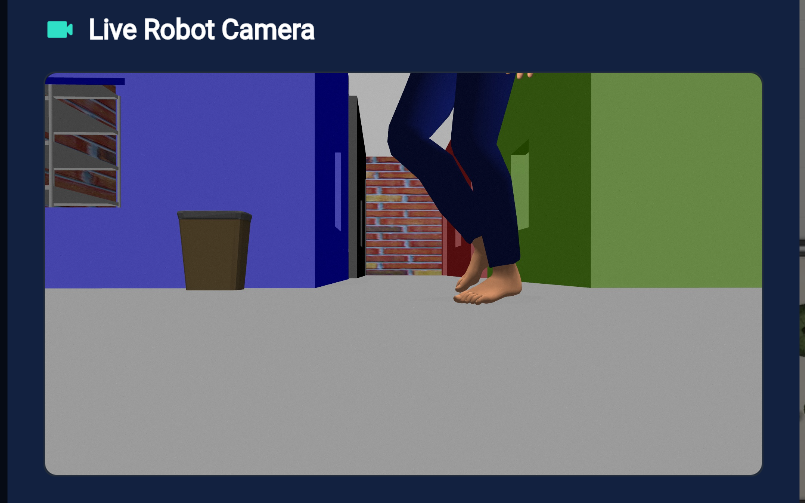
\includegraphics[width=0.6\textwidth]{live_robot_camera.png}
	\caption{Live robot camera feed displayed through the administrator interface.}
	\label{fig:live_camera}
\end{figure}

The live RGB camera feed received by the robot during its navigation in the delivery environment is shown in figure~\ref{fig:live_camera}. The administrator can see what the robot is doing in the current area, such as corridors, room entry points and other people who are close by the robot so that the delivery process can be constantly monitored. This ability adds an extra layer of operational awareness and helps in verifying safe autonomous navigation throughout the mission.

\section{Phase 5: ROS 2 and Gazebo Simulation Results}

In the last phase, all the previously validated planning and control algorithms were transferred to a completely integrated ROS~2 and Gazebo simulation. This milestone is the first time that we have successfully implemented the full stack of SLAM, simulated LiDAR and camera sensing, and our own IA*-based global planner, pruner, spline smoother and MPC controller pipeline in a custom ROS~2 node, and autonomously executed parcel delivery missions within a custom multi-room indoor world, without using any navigation planner.

\subsection{Custom Multi-Room Delivery Environment}
A realistic multi-room environment, like an office floor, was replicated in Gazebo, an indoor world created specifically for the project. The environment is made up of five different rooms, each given a colour coding red, green, grey, blue and teal with a central corridor linking all the rooms and an outer boundary wall. Each room has only one portal to the corridor and the robot can only enter the room through one protected portal, as in a real indoor delivery.\begin{figure}[H]
	\centering
	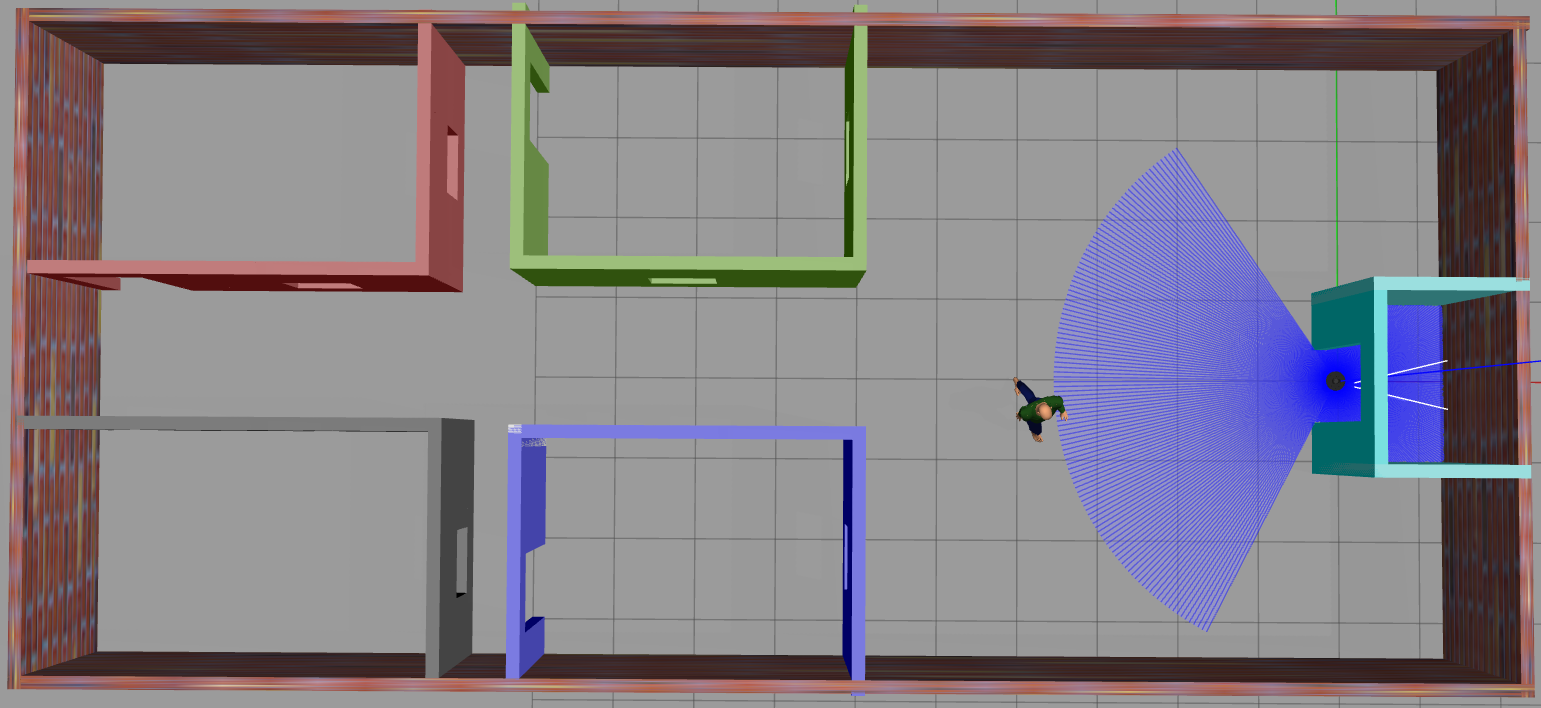
\includegraphics[width=0.9\textwidth]{gazebo_world.png}
	\caption{view of the multi-room Gazebo delivery environment}
	\label{fig:gazebo_world}
\end{figure}

Figure~\ref{fig:gazebo_world} shows the base layout viewed from above. The robot's 360-degree LiDAR footprint appears as the blue fan-shaped region, confirming that the simulated scanner correctly registers the surrounding walls and corridor space. A walking human actor near the robot was scripted to move across the corridor as an unpredictable dynamic obstacle.

The rooms were further populated with furniture models, including sofas, chairs, desks, filing cabinets, a vending machine, and a parked utility vehicle outside the building. This furnished world, shown in Figure~\ref{fig:gazebo_furnished}, was used for all subsequent trials, since it adds static clutter that the planners must account for.

\begin{figure}[H]
	\centering
	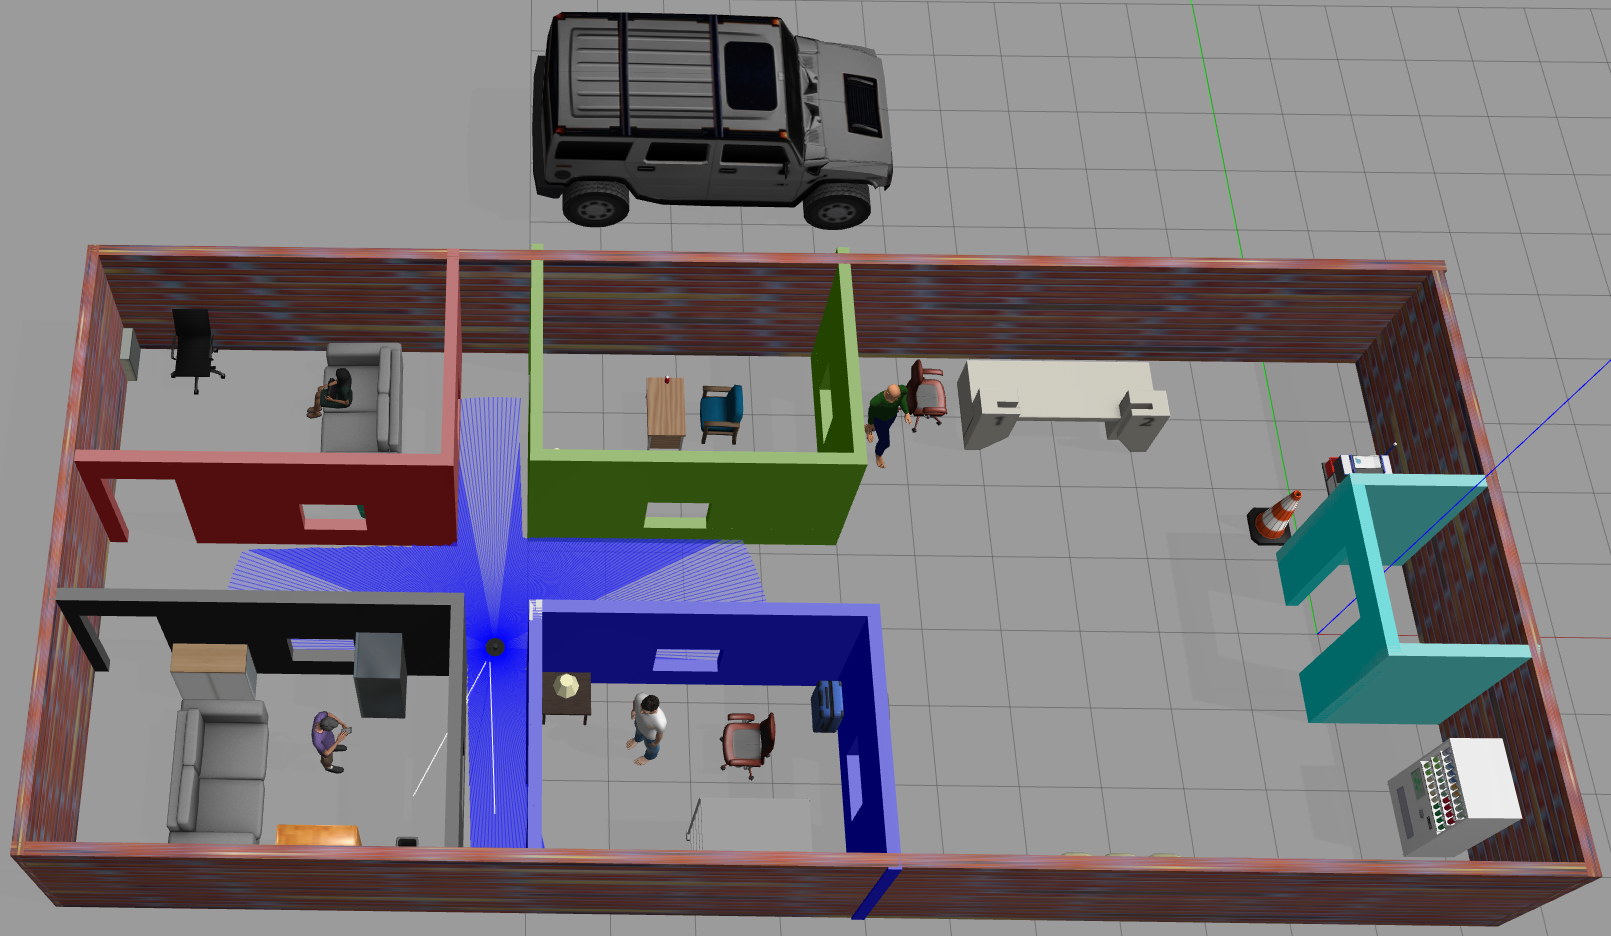
\includegraphics[width=0.9\textwidth]{In_middle_of_delivery.png}
	\caption{Isometric view of the fully furnished delivery environment}
	\label{fig:gazebo_furnished}
\end{figure}

\subsection{Reference Floor Plan}

The room arrangement, door locations, and corridor widths were planned using a simplified two-dimensional floor plan prior to the construction of the world in Gazebo. The zoning is color-coded in this schematic, which is displayed in Figure~\ref{fig:2dmap}. Yellow denotes the two enclosed side rooms, green the two mid-corridor rooms, and blue the open corridor and delivery area that connects them. When positioning walls and doors in the Gazebo world files, it served as a direct reference.


\begin{figure}[H]
	\centering
	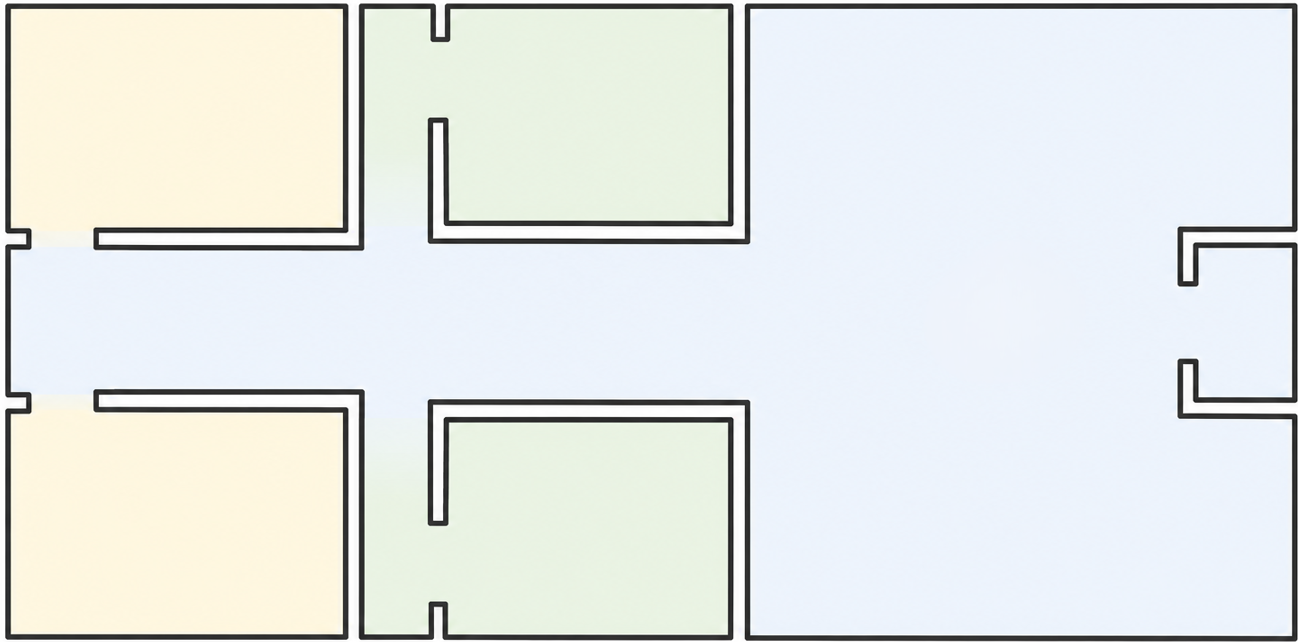
\includegraphics[width=0.9\textwidth]{2d_map_of_world.png}
	\caption{Reference 2D floor plan used to design the room layout of the Gazebo world}
	\label{fig:2dmap}
\end{figure}

\subsection{SLAM-Based Occupancy Mapping}

With the world constructed, the robot was driven through the environment using ROS~2's SLAM stack, based on LiDAR scan matching, to autonomously build a 2D occupancy grid map. The resulting map, shown in Figure~\ref{fig:slam}, closely mirrors the reference floor plan of Figure~\ref{fig:2dmap}, correctly reconstructing every wall, doorway, and room boundary from raw sensor data. The small outlines inside each room correspond to the furniture pieces, confirming the LiDAR resolves obstacles with enough detail for downstream planning, and the red marker denotes the robot's estimated pose.

\begin{figure}[H]
	\centering
	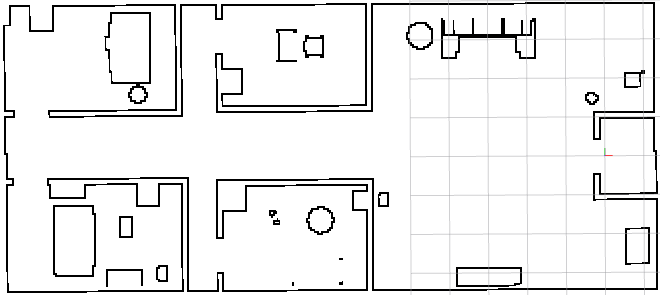
\includegraphics[width=0.85\textwidth]{Slam_output_of_world_with_objects.png}
	\caption{Occupancy grid map generated through SLAM}
	\label{fig:slam}
\end{figure}

This SLAM-generated map was saved and supplied directly to our own path-planning nodes as the static map, on top of which the same obstacle inflation strategy developed in Phase 3 was applied to build the inflated planning map used for the global path search.


\subsection{Path Planning and Smoothing in RViz}



To validate the planning and smoothing pipeline under realistic conditions, a test was conducted in a cluttered obstacle environment. The generated global path was inflated around obstacle boundaries to maintain a safe clearance margin, after which the raw IA* path was refined using the pruning and PSO-based smoothing stages. The pipeline then generated a planning map (Figure~\ref{fig:planning_smoothing_test}) that was inflated, a initial planned path, and a final smoothed planning path while navigating through the obstacle dense environment.

\begin{figure}[H]
	\centering
	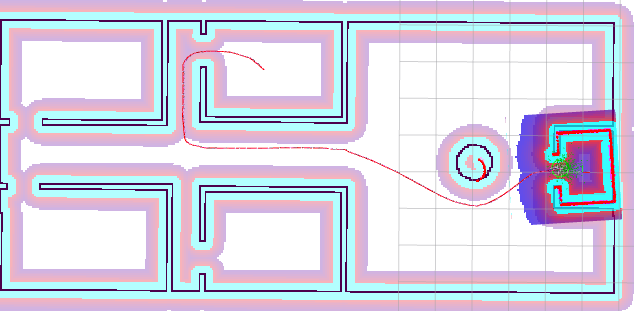
\includegraphics[width=0.6\textwidth]{di.png}
	\caption{Path Planning and Smoothing Test Under an Obstacle Environment}
	\label{fig:planning_smoothing_test}
\end{figure}

The results show that the planner is able to generate the route that does not collide with the obstacles while maintaining the inflated safety margins and the smoothing stage results in a continuous trajectory that is suitable for the motion controller.
Once localized within the SLAM-generated map, the robot was assigned a pickup goal, and the resulting inflated planning map, planned path, and smoothing behaviour produced by our own IA*, pruning, and spline-smoothing pipeline were visualized in RViz. Figure~\ref{fig:rviz_planning} shows the obstacle-inflated map overlaid on the static map, where the light pink region is the inflation buffer and the cyan outline marks the true obstacle boundaries. The red trace shows the path generated by our global planner and refined by the smoothing stage, while the small spiral near the goal is a brief in-place recovery rotation performed by our MPC controller to correct heading before the final approach.

\begin{figure}[H]
	\centering
	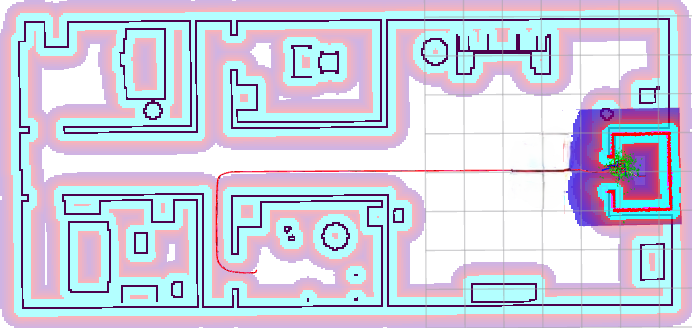
\includegraphics[width=0.85\textwidth]{rviz_p.png}
	\caption{RViz visualization of planned path, and smoothing behaviour produced by custom path-planning pipeline while the robot approaches the pickup location}
	\label{fig:rviz_planning}
\end{figure}

The pruning and smoothing pipeline validated earlier in Section 5.1, Step 4, carried over correctly into the full ROS~2 integration, producing trajectories that remain collision-free and remain practically followable by our own MPC controller, as confirmed by the clean, continuous curvature of the path through the narrow corridor sections.


\subsection{Dynamic Obstacle Avoidance}
A human actor was given instructions to stroll across the robot's intended delivery route while it was navigating toward its destination in order to assess the robustness of the suggested navigation framework in dynamic interior situations.
The experiment is presented in a top-down view in Figure~\ref{fig:person_avoidance} where the robot's LiDAR continually scans the environment around him and detects the moving pedestrian when it enters into the environment's sensing range.

The robot first follows the globally optimized path which was computed using the A* algorithm, then the path is pruned and then smoothed using PSO. Upon detecting the pedestrian, the MPPI (Model Predictive Path Integral) controller predicted multiple short-horizon feasible trajectories in real-time based on the measured LiDAR data, while accounting for obstacle clearance, path tracking precision and smoothness of the motion. The controller chose the path of the lowest cost to avoid collisions, with the robot temporarily off of the path of the original global path, but still navigating safely around the moving obstacle.

Once the pedestrian was out of the robot's way, the obstacle was deleted from the local cost map and the MPPI controller took the robot back to the smoothed global trajectory. The global path was valid and no global replanning was needed. With this local trajectory optimization, collision-free, smooth, continuous navigation towards the delivery target was achieved without any manual inputs.

\begin{figure}[H]
	\centering
	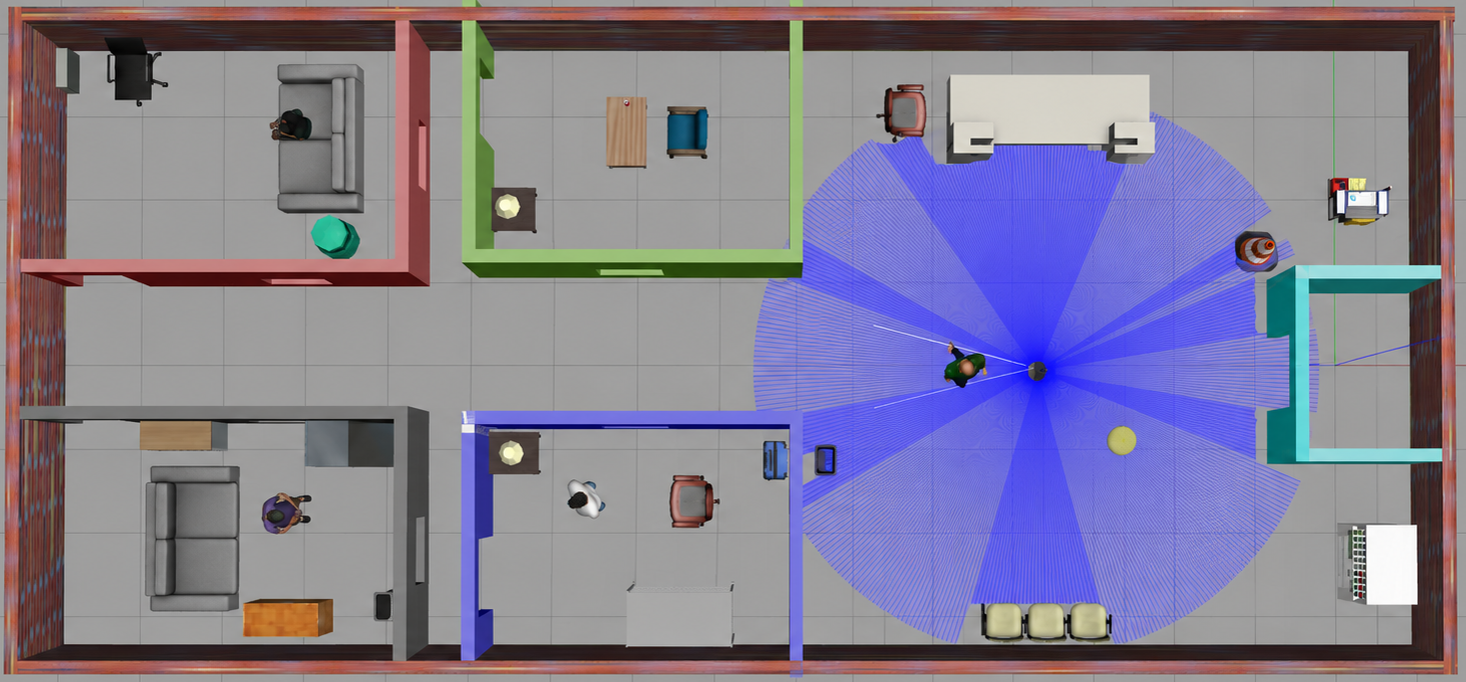
\includegraphics[width=0.9\textwidth]{person_avoidance_during_delivery.png}
	\caption{Robot detecting and safely avoiding a moving pedestrian during a parcel delivery task.}\label{fig:person_avoidance}
\end{figure}
\subsection{Arrival at the Delivery Point}

Once the robot reaches its delivery room, it is seen in Figure~\ref{fig:delivery_point}. The robot has stopped at the designated goal location once it enters the authorized drop-off area. The objective coordinate (obtained from the web interface) was successfully converted into the map frame, and the robot went through the environment safely, without colliding with any obstacles, as evidenced by the successful arrival.

\begin{figure}[H]
	\centering
	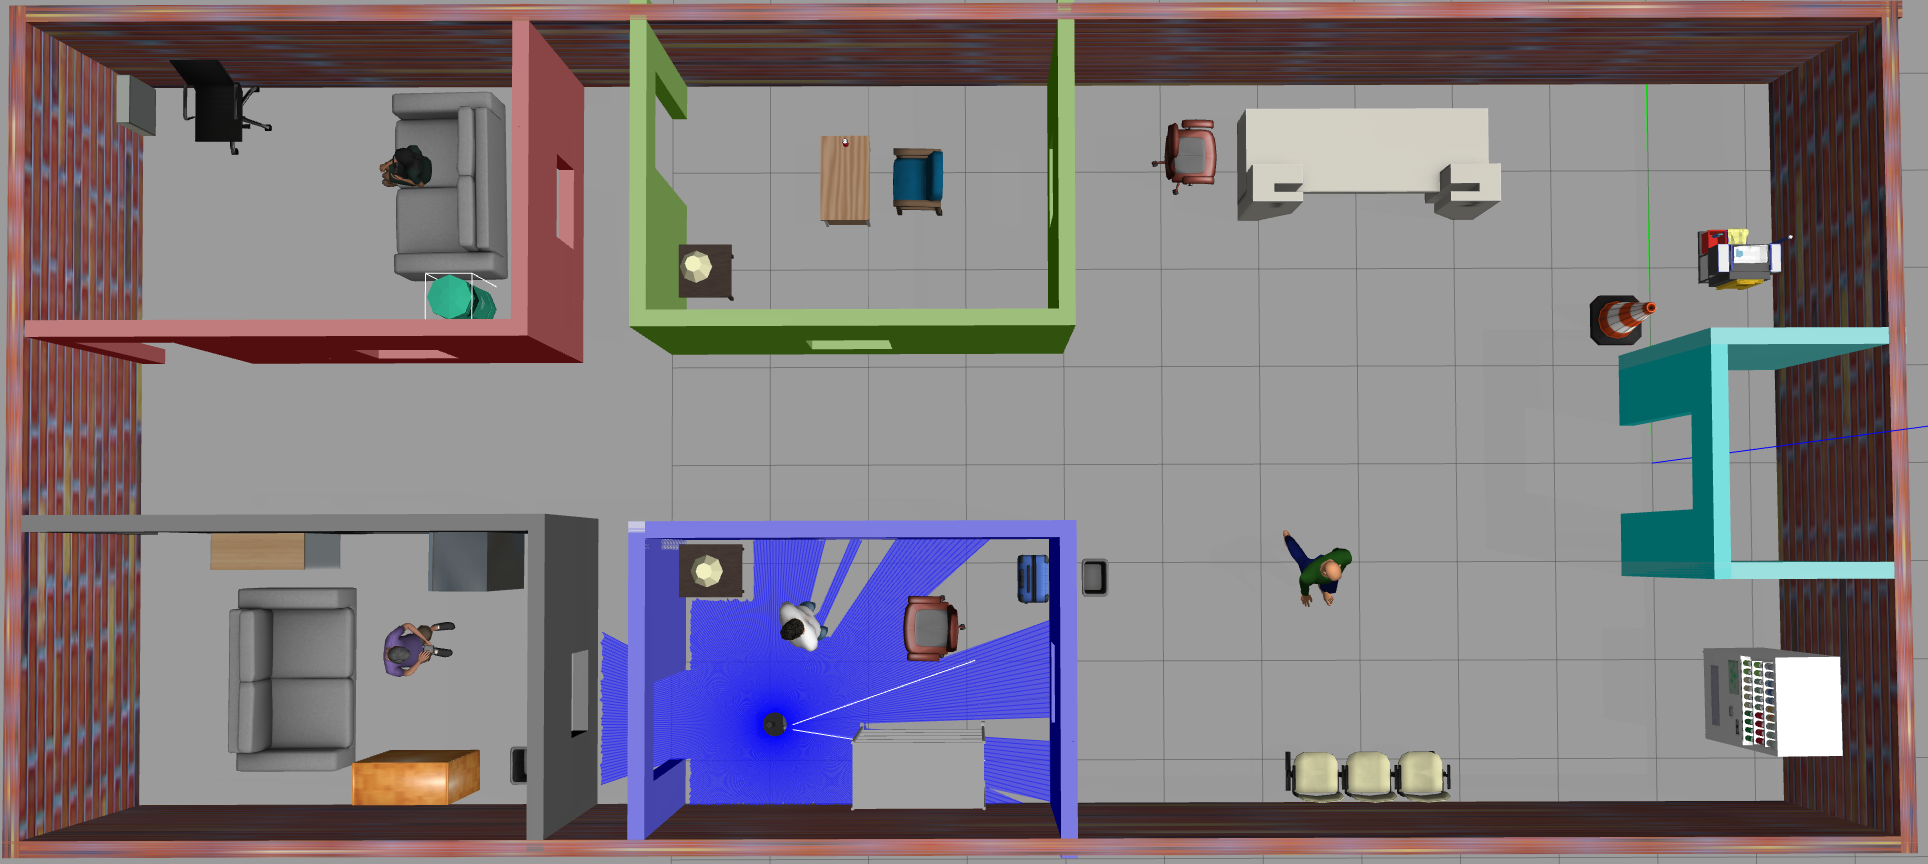
\includegraphics[width=0.9\textwidth]{gazebo_marking_robot_at_delivery_point.png}
	\caption{Robot arriving at the designated delivery point inside the drop-off room}
	\label{fig:delivery_point}
\end{figure}

\subsection{Complete Delivery Mission}

Lastly, the RViz visualization following a successful end-to-end parcel delivery mission is shown in Figure~\ref{fig:rviz_complete}. While the MPPI controller continually carried out local trajectory optimization to safely avoid dynamic impediments as they were met, the robot began at the pickup site and followed the globally optimized trajectory created using the A* algorithm, route trimming, and PSO-based path smoothing. The trajectory that is shown shows the entire path that the robot took, ending at the specified delivery location. The mission's successful conclusion shows how global path planning, path optimization, local obstacle avoidance, and autonomous navigation may be seamlessly integrated to enable dependable end-to-end parcel delivery without the need for human intervention.

\begin{figure}[H]
	\centering
	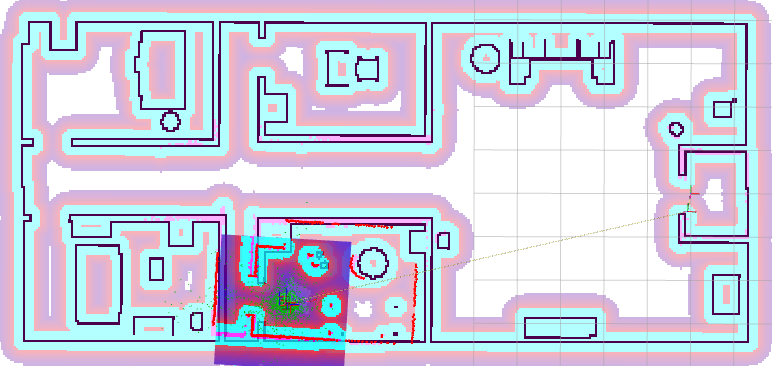
\includegraphics[width=0.85\textwidth]{rviz_showing_complete_delivery.png}
	\caption{RViz visualization confirming successful completion of the full delivery mission from pickup to drop-off}
	\label{fig:rviz_complete}
\end{figure}

Together, these results demonstrate the successful integration of the proposed navigation framework, consisting of SLAM-based mapping, obstacle inflation, A*-based global path planning, path pruning, PSO-based path smoothing, MPPI-based local trajectory optimization, and LiDAR-based dynamic obstacle avoidance. In the ROS~2 and Gazebo environments, the suggested system successfully completed end-to-end parcel delivery missions, precisely moving across several rooms while securely avoiding both static and dynamic impediments. These outcomes confirm that the suggested navigation architecture for autonomous interior parcel delivery is reliable and efficient.


\section{Limitations of the Working Prototype}

The functioning prototype has a number of drawbacks, despite the suggested navigation framework's dependable performance in the ROS~2 and Gazebo simulations. Since the complete system was only tested in simulation, it hasn't been verified on a real robot with sensors, motors, and network hardware, where performance could be impacted by noise, latency, and mechanical flaws. The robustness of dynamic obstacle avoidance in busier, more chaotic contexts is yet unknown because it was evaluated against a single planned pedestrian rather than several, erratic human movements. Additionally, because the system depends on a manually specified floor plan and a pre-built SLAM map, it is currently unable to automatically adjust to changes in the environment, such as rearranging rooms or moving furniture.
Additionally, the existing design only allows one robot at a time and lacks a system for managing shared passageways or coordinating several robots. Lastly, as they are outside the purview of a simulation-based prototype, issues like battery life, charging, and long-term autonomous operation were not covered.

\section{Challenges Faced}

Several technical difficulties arose during the implementation and integration of several software components during the autonomous parcel delivery system's development. Before a solid and dependable system was created, these difficulties necessitated a great deal of debugging, parameter adjusting, and iterative testing.\begin{itemize}
     \item \textbf{Obstacle Collision During Path Planning:}
	In the initial stages of path planning some projected paths were too close to the obstacles and could lead to a potential collision. Obstacle inflation and definition of safe margins allowed the robot to safely navigate to the destination.


\item \textbf{Path Smoothing Issues:}
The paths generated by the Improved A* algorithm were not only not collision free, but had sharp turns that were difficult to follow smoothly by the robot. The cubic spline interpolation was used to produce smoother curves and maintain a safe distance from obstructions. There was a few iterations to get the balance between path accuracy and smoothness right.

\item \textbf{Gazebo Installation and Simulation Setup:}
The setup of Gazebo simulation environment was one of the initial challenges faced by the project. In rare cases, there were rendering and resources setting issues, which lead to black screen or world not loading. These problems were resolved by selecting the right rendering engine, ensuring the paths for resources were set up correctly, and installing the dependencies.


\item \textbf{Custom World Development:}
It was necessary to build rooms, hallways, furniture, doors, and moving human actors while making sure the robot had enough area to move about securely in order to create a realistic indoor setting. A series of changes in the size of the items, collision properties, and placement of the models was made until a steady simulation environment was achieved.

\item \textbf{Motion Controller (MPC) Tuning:}
The first problem with this robot is that it was initially having trouble following the paths accurately generated by the global planner. To enable the robot to follow the intended course in different scenarios, the MPC controller required fine tuning of prediction horizons, weights on the control and velocity limitations.


\item \textbf{ROS~2 and Web Application Integration:}
A major challenge was to integrate the Flutter web application into the ROS~2 navigation system. Reliable communication between the Flutter frontend, the Flask backend and the ROS~2 nodes was necessary to send delivery requests, receive robot status information and accurately display real information.


\item \textbf{Package Dependency Conflicts:}
During installation and upgrades, the project's use of multiple ROS~2 packages and third-party libraries occasionally resulted in dependency conflicts. Installing suitable package versions and recreating the workspace as needed fixed these problems.


\item \textbf{Launch File Configuration:}
The system became more complicated due to the need to manage several launch files for Gazebo, SLAM Toolbox, Nav2, the Flask backend, and custom ROS~2 nodes. To make sure that every component began in the right order and functioned as intended, careful planning and frequent testing were necessary.

\item \textbf{System Integration and Testing:}
Integrating all of the system's components path planning, motion control, SLAM, Gazebo, ROS~2, the Flask backend, and the Flutter web application—into a single functional system was the last obstacle. To ensure that the robot could successfully fulfill delivery missions from beginning to end and that all modules communicated appropriately, extensive testing was conducted.


\end{itemize}

Despite these difficulties, a fully integrated autonomous package delivery system with dependable navigation, obstacle avoidance, and real-time user engagement via the web application was produced through constant debugging, parameter tuning, and repetitive testing.

% ══════════════════════════════════════════════════════════════════════════════

\section{Summary}
The design, execution, and assessment of the suggested Autonomous Parcel Delivery System were covered in this chapter through a number of progressive development phases. When the A* algorithm was originally used for global path planning, it produced paths inside the occupancy grid map that were free of collisions. To create shorter, smoother, and robot-friendly trajectories appropriate for autonomous navigation, path trimming and PSO-based smoothing were then used.Obstacle inflation ensured safe planning around static impediments, and a web-based interface was created to allow users to designate pickup and delivery locations.An MPPI controller was specially used to avoid dynamic impediments by carrying out real-time local trajectory optimization based on LiDAR readings, while an MPC controller precisely followed the optimized global trajectory for path execution.
Ultimately, these elements were combined to create a realistic multi-room delivery scenario with pedestrians traveling across the ROS~2 and Gazebo simulation environments. The TurtleBot3 successfully produced a SLAM map, streamed real-time sensor data, planned and optimized collision-free routes, used the MPPI controller to avoid dynamic obstacles, and finished delivery tasks from pickup to drop-off. The results justify the effectiveness and reliability of the proposed navigation system for autonomous interior package delivery.

	\chapter{Conclusion and Future Work}

\section{Conclusion}

This project presented the design and implementation of a User-Friendly Autonomous Parcel Delivery System with Adaptive Navigation aimed at addressing the growing demand for efficient and intelligent indoor logistics solutions. The system was developed entirely in a simulation environment using ROS~2 and Gazebo, focusing on reliable navigation, intelligent path planning, and smooth trajectory execution so that robot does not have to slow down during turns and effiently aviod any walking person.

The primary objective of the project was to design a mobile robot capable of navigating structured indoor environments such as university buildings and office corridors while safely avoiding obstacles and delivering parcels to specified goal locations.It can also be placed in special enivornemnts like isolation wards or hospital to avoid virus transmission. This objective was successfully achieved through the integration of an Improved A* (IA*) algorithm for global path planning, cubic spline interpolation for trajectory smoothing, and a Model Predictive Control (MPC) strategy for accurate motion tracking.

Different path planning algorithms were studies but he Improved A* algorithm proved effective in generating collision-free and near-optimal paths on grid maps. The addition of obstacle inflation and waypoint pruning enhanced both safety and computational efficiency. Since grid-based planners naturally produce piecewise-linear paths with sharp turns, spline-based smoothing was applied to generate continuous and kinematically feasible trajectories suitable for differential-drive robotsso so that does not have to slow down during curves and effiently aviod any walking person. The MPC controller ensured stable and accurate tracking of these trajectories across different simulated environments.

All the system was deployed in the context of the ROS 2 with the use of modular nodes and traditional communication patterns. A web-based control interface was also designed simultaneously to allow users to define delivery goals, simulate the spatial environment, and track the actions of the robot in real time. Extensive testing also revealed that the robot is able to navigate complicated indoor setups, avoid obstacles and get to the predefined target points with a good degree of consistency.

On the whole, it can be concluded that the project has achieved its desired goals and supported the fact that simulation-based development is a powerful and safe approach to the development of autonomous delivery systems. The article provides a strong background of further research and practical implementation of smart indoor logistics robots.

\section{Future Work}
 As much as the proposed system has demonstrated good performance in the simulated indoor settings, there are yet to be explored promising research directions. Those extensions might increase the intelligence, scalability and usefulness of the system in real world significantly.

\begin{itemize}
    \item \textbf{Real-World Deployment and Sensor Fusion:}  
 One of the major follow-up tasks is to transfer the system to a real robot. It implies connecting real sensors LiDAR, RGB -D cameras, IMUs, wheel encoders, etc. With this advanced sensor fusion, e.g. Extended Kalman Filters or factor-graph SLAM, the robot should be able to more accurately localise itself in the presence of all the real-world noises and uncertainty.
 
    \item \textbf{Learning-Based Navigation and Decision Making:}  
  As much as the proposed system has demonstrated good performance in the simulated indoor settings, there are yet to be explored promising research directions. Those extensions might increase the intelligence, scalability and usefulness of the system in real world significantly.
  
  The next generation implementation may incorporate reinforcement learning or imitation learning to enable the robot to gain navigation policies by experience. That would allow it to be more adaptive to complex and crowded environments.
    \item \textbf{Multi-Robot Coordination:}  
   We can totally scale it, Hey, we could run a number of delivery robots, at a time. It would then be necessary to determine how to divide work among them, establish a manner of them communicating with each other, and coordinate their pathways. It would make the entire process much more efficient in large institutions such as hospitals or college campuses.
   
  
    \item \textbf{Semantic Mapping and Context-Aware Navigation:}  
  
  The inclusion of semantic SLAM would enable the robot to actually see things such as doors, elevators, people, furniture so it can tag them. Knowing that, the robot may make more intelligent and higher level decisions and maintain itself around people safer.
  
    \item \textbf{Dynamic Global Replanning and Prediction:}  
 
 We can also predictively global replan in future, so the robot will actually guess where people are heading and dynamically adjust its route on the fly according to the changing environment.
 

    \item \textbf{Human--Robot Interaction (HRI):}  
   Lastly, in case we add voice commands, phone-to-phone push notifications, and certain visual feedback, the system would be much more friendly and more acceptable in daily environments.
   
    \item \textbf{Energy-Aware and Sustainable Navigation:}  
     Autonomous charging plans can be combined with energy-efficient path planning to allow the robotic systems to operate sustainably and over a long period.
    
    \item \textbf{Cloud and IoT Integration:}  
   The integration of the system with cloud services as well as the IoT infrastructure would allow tracking the fleet, analyzing the data in real-time, and improving it on the basis of the actual data related to the real operation.
\end{itemize}

	\chapter{SUSTAINABLE DEVELOPMENT GOALS (SDGs)}

\section{Overview of SDGs}

The United Nations approved the Sustainable Development Goals (SDGs) popularly known as the Global Goals in 2015 as a universal call to end poverty, protect the planet and secure peace and prosperity to all by the year 2030. These 17 goals are closely connected, and it should be emphasized that the accomplishment of one field inevitably affects the results in other areas, and to achieve the real sustainability, the social, economic and environmental aspects should be considered with the necessary equilibrium.
	
	Engaging in the sphere of engineering research and development, the understanding of how a technical solution promotes the solution of the global issues is the primary concern. This project is called User-Friendly Autonomous Parcel Delivery System with Adaptive Navigation; it corresponds to several SDGs because it successfully incorporates robotics and intelligent automation into the world of healthcare, education, and industrial infrastructure.
\begin{figure}[H]
	\centering
	
\includegraphics[width=0.85\textwidth]{SDGs.png}
	\caption{United Nations 17 Sustainable Development Goals Framework~\cite{un2015sdgs}}
	\label{fig:sdg_overview}
\end{figure}

\section{Alignment of Project with SDGs}

\subsection{SDG 3: Good Health and Well-Being}

The healthcare industry is one of the main areas of application of the suggested autonomous delivery system. The SDG~3 is relevant to the project in the following ways:

\begin{itemize}
	\item \textbf{Infection Control:}
	
	The robot can transport medicines, laboratory samples, and medical supplies without involving human movements, which is why it reduces the needless human movement in the high-risk areas and, consequently, minimizes the chances of cross-contamination and transmitting infectious diseases.
	
	\item \textbf{Operational Efficiency:} 	Relocating logistical duties that are repetitive to the healthcare workers will enable them to pay more attention to the patients, lessening the workload burden and enhancing the overall health services quality.
	
	\item \textbf{Safety in Medical Logistics:}	The system guarantees a regulated and trusted approach of handling sensitive materials as well as the integrity of samples and forms of transport.
\end{itemize}

\begin{figure}[H]
	\centering
	
\includegraphics[width=0.3\textwidth]{sdg3.png}
	\caption{SDG 3: Good Health and Well-Being}
	\label{fig:sdg3_health}
\end{figure}

\subsection{SDG 4: Quality Education}

The proposed system also supports SDG~4 by enhancing operational efficiency and learning opportunities within educational institutions:

\begin{itemize}
	\item \textbf{Campus Automation:} 
	The robot also helps in the transportation of documents, books, and laboratory equipment across the various departments, enhancing the logistics in the institution and minimizing the administration delays.
	
	\item \textbf{Practical Engineering Application:} 
	Being a research based project, it is an effective tool that enables the learner to learn ROS~2, autonomous navigation, and path planning, which is a gap between theory and practice.
\end{itemize}

\begin{figure}[H]
	\centering
	
\includegraphics[width=0.3\textwidth]{sdg4.png}
	\caption{SDG 4: Quality Education ~\cite{unsdg4}}
	\label{fig:sdg4_education}
\end{figure}

\subsection{SDG 9: Industry, Innovation, and Infrastructure}

Innovation and infrastructure development form the core of this Final Year Project (FYP). The proposed system contributes to SDG~9 in the following ways:

\begin{itemize}
		\item \textbf{Technological Advancement:} Application of the Robot Operating System (ROS 2) and new perception devices including LiDAR and RGB-D cameras is an important milestone towards intelligent and autonomous internal logistics.
		
	
	\item \textbf{Scalable Industrial Solutions:} 
	
	The modular structure enables both large-scale warehouse, hospital, and industrial facilities deployments as well as supporting robust and innovative infrastructures.
	
		
	\item \textbf{Efficiency in Logistics:}	The system enhances reliability or productivity within the commercial and industrial settings by minimizing human error and manual handling of products when it comes to indoor transportation.
	
\end{itemize}

\begin{figure}[H]
	\centering
	
\includegraphics[width=0.3\textwidth]{sdg9.png}
	\caption{SDG 9: Industry, Innovation and Infrastructure }
	\label{fig:sdg9_innovation}
\end{figure}

\subsection{SDG 11: Sustainable Cities and Communities}

The project supports the vision of smart and sustainable communities through intelligent automation.

\begin{itemize}
	\item \textbf{Smart Campus and Office Integration:} 
	The automation of in-door delivery allows reducing the human overload on the system, and enhances workplace and learning area organization.
	
	
	\item \textbf{Sustainable Resource Management:} 
	The electric robotic platform that is run by battery reduces the carbon footprint to the traditional methods of transport which use either manual or fuel-powered methods which helps in creating cleaner and sustainable living environments.
	
\end{itemize}

\begin{figure}[H]
	\centering
	
\includegraphics[width=0.3\textwidth]{sdg11.png}
	\caption{SDG 11: Sustainable Cities and Communities~\cite{unsdg11}}
	\label{fig:sdg11_cities}
\end{figure}

\section{Implementation Summary Table}

Table~\ref{tab:sdg_implementation} summarizes the key contributions of the proposed system to the targeted Sustainable Development Goals.

\begin{table}[H]
	\centering
	\caption{Project Alignment with Sustainable Development Goals}
	\label{tab:sdg_implementation}
	\begin{tabular}{|c|p{4cm}|c|p{6.5cm}|}
		\hline
		\textbf{Sr. No} & \textbf{Targeted SDGs} & \textbf{Goal No.} & \textbf{Implementation Detail} \\
		\hline
		1 & Good Health \& Well-Being & SDG~3 & Reduces human contact in hospitals by autonomously transporting medicines and laboratory samples, minimizing cross-contamination. \\
		\hline
		2 & Quality Education & SDG~4 & Supports university logistics and provides a practical research platform for autonomous robotics and ROS~2-based learning. \\
		\hline
		3 & Industry, Innovation \& Infrastructure & SDG~9 & Implements a scalable ROS~2-based architecture for modernizing internal logistics in commercial and industrial sectors. \\
		\hline
		4 & Sustainable Cities \& Communities & SDG~11 & Promotes the ``Smart Campus'' concept by reducing indoor congestion and improving delivery efficiency through automation. \\
		\hline
	\end{tabular}
\end{table}

\section{Chapter Summary}

This chapter showed the socio-economic and environmental applicability of the suggested Autonomous Delivery Robot by matching it with the United Nations Sustainable Development Goals. The project can achieve SDG~3, SDG~4, SDG~9, and SDG~11, which makes it much more than a technical prototype, but a sustainable and socially responsible project. This direction will see the project go in line with the worldwide vision of safe healthcare systems, quality education, innovative industries, and smart and sustainable communities.

	\bibliographystyle{IEEEtran}
	
	\renewcommand{\bibname}{References}
	
	\bibliography{references}
	%\include{appendixA}
	%\include{appendixB}
	%\include{appendixC}
	
\end{document}